% concatenated from main.tex
\documentclass{amsart}
 

\usepackage{graphicx,color}
\usepackage{euscript}
\usepackage{amsmath}
\usepackage{amsfonts}
\usepackage{amssymb}
\usepackage{amsthm}
\usepackage{hyperref}
\usepackage{epsfig}
\usepackage{epsf}
\usepackage{epstopdf}
\usepackage{caption}
\usepackage{url}
\usepackage{array}
\usepackage{amssymb}\usepackage{amscd}
\usepackage{epic}
\usepackage{eufrak}
\usepackage{tikz,underscore,pgfplots}
\usepackage{tikz-cd}
\usepackage{bm}
\usepackage{float}
\usepackage{anysize}
\usepackage{amsfonts}
\usepackage{pinlabel} 
\usepackage{combelow}
\usepackage{comment}


%\graphicspath{{figs/}}




 
\newtheorem{theorem}{Theorem}[section] 
\newtheorem{corollary}[theorem]{Corollary} 
\newtheorem{lemma}[theorem]{Lemma} 
\newtheorem{proposition}[theorem]{Proposition} 
\newtheorem{example}[theorem]{Example}
\newtheorem{conjecture}[theorem]{Conjecture}
\newtheorem{problem}[theorem]{Problem}  
\newtheorem{remark}[theorem]{Remark}  
\newtheorem{definition}[theorem]{Definition}
\newtheorem{algorithm}[theorem]{Algorithm}
 

\newcommand{\ch}{\mathrm{char}}

\newcommand{\Kh}{\mathrm{Kh}}

\newcommand{\CA}{\mathcal{A}} 
\newcommand{\CH}{\mathcal{H}}
\newcommand{\Cab}{\mathrm{Cab}}
\newcommand{\col}{\mathrm{col}}
\newcommand{\Tw}{\mathcal{TW}}

\newcommand{\F}{\mathbb{F}}
\newcommand{\E}{\mathbf{E}}
\newcommand{\C}{\mathbb{C}}
\newcommand{\CC}{\mathcal{C}}
\newcommand{\cCFL}{\mathcal{C\!F\!L}}
\newcommand{\cCFK}{\mathcal{C\hspace{-.5mm}F\hspace{-.3mm}K}}
\newcommand{\cHFL}{\mathcal{H\!F\! L}}
\newcommand{\CFL}{\mathit{CFL}}
\newcommand{\HFL}{\mathit{HFL}}
\newcommand{\HFK}{\mathit{HFK}}
\newcommand{\HF}{\mathit{HF}}
\newcommand{\Cone}{\mathrm{Cone}}
\newcommand{\scU}{\mathscr{U}}
\newcommand{\scV}{\mathscr{V}}
\newcommand{\s}{\mathfrak{s}}
\newcommand{\ee}{\mathbf{e}}
\newcommand{\ff}{\mathbf{f}}
\newcommand{\full}{\mathrm{full}}
\newcommand{\sgn}{\mathrm{sgn}}
\newcommand{\lk}{\mathrm{lk}}
\newcommand{\Split}{\mathrm{split}}
\newcommand{\Spin}{\text{Spin}^{c}}
\newcommand{\alphas}{\boldsymbol{\alpha}}
\newcommand{\betas}{\boldsymbol{\beta}}
\newcommand{\gammas}{\boldsymbol{\gamma}}
\newcommand{\deltas}{\boldsymbol{\delta}}
\newcommand{\ovl}{\overline}

\newcommand{\cbHFL}{\boldsymbol{{\mathcal{H\!F\!L}}}}
\newcommand{\cbCFL}{\boldsymbol{\mathcal{C\!F\!L}}}
\newcommand{\bJ}{\boldsymbol{\J}}

\newcommand{\Imm}{\mathrm{Im}}
\newcommand{\cK}{\mathcal{K}}
\newcommand{\bt}{\mathbf{t}}
\newcommand{\HD}{\mathcal{H}}
\newcommand{\G}{\mathcal{G}}
%\newcommand{\i}{\mathit{in}}

\newcommand{\tw}{\mathbf{tw}}
\newcommand{\w}{\mathbf{w}}
\newcommand{\x}{\mathbf{x}}
\newcommand{\y}{\mathbf{y}}

\newcommand{\newword}[1]{\emph{\textbf{#1}}}

\newcommand{\spinc}{\text{Spin}^{c}}


\newcommand{\Alt}{\mathrm{Alt}}
\newcommand{\HY}{\mathrm{HY}}

\def\L{\mathcal{L}}
\def\gr{\textup{gr}}
\def\w{{\bf{w}}}
\def\z{{\bf{z}}}
\def\d{\mathbf{d}}
\def\x{\mathbf{x}}
\def\y{\mathbf{y}}

\def\k{\mathbf{k}}
\def\m{\mathbf{m}}
\def\bF{\mathcal{F}}


\newcommand{\HHH}{\mathrm{HHH}}

\newcommand{\FT}{\mathrm{FT}}

\newcommand{\HH}{\mathbb{H}}
\newcommand{\Z}{\mathbb{Z}}
\newcommand{\R}{\mathbb{R}}
\newcommand{\UU}{\mathbf{U}}
\newcommand{\A}{\mathfrak{A}}
\newcommand{\CT}{\mathcal{T}}

\newcommand{\Br}{\mathrm{Br}}

\newcommand{\J}{\mathcal{J}}

\renewcommand{\AA}[1]{{\color{blue}#1}}
\newcommand{\EG}[1]{{\color{red}#1}}
\newcommand{\BL}[1]{{\color{purple}#1--Beibei}}
%\def\aa#1{{\textcolor{blue}{#1}}}

\newcommand{\spl}{\mathrm{sp}}

\newcommand{\cc}{\mathbf{c}}

\newcommand{\ttt}{\mathbf{t}}

\newcommand{\GCD}{\mathrm{GCD}}
\newcommand{\CFK}{\mathrm{CFK}}
\newcommand{\CF}{\mathcal{F}}

\newcommand{\Id}{\mathrm{Id}}

\newcommand{\spann}{\mathrm{span}}

\newcommand{\stab}{\mathrm{stab}}

\renewcommand{\ss}{\mathbf{s}}

\newcommand{\AAA}{\mathsf{A}}


\title{Colored knot Floer homology: structures and examples}



\author{Akram Alishahi}
\thanks{\texttt{AA was partly supported by NSF Grant DMS-2238103}}
\address{Department of Mathematics, University of Georgia, Athens, GA 30602 USA}
\email{\href{mailto:akram.alishahi@uga.edu}{akram.alishahi@uga.edu}}

\author{Eugene Gorsky}
\thanks{\texttt{EG was partly supported by NSF Grant DMS-2302305}}
\address{Department of Mathematics, University of California Davis\\ One Shields Avenue, Davis CA 95616 USA}
\email{\href{mailto:egorskiy@ucdavis.edu}{egorskiy@ucdavis.edu}}


\author{Beibei Liu}
\thanks{\texttt{BL was partly supported by NSF Grant DMS-2417229}}
\address{Department of Mathematics, The Ohio State University, 100 Math Tower, 231 W 18th Ave, Columbus, OH 43201 USA}
\email{\href{mailto:liu.11302@osu.edu}{liu.11302@osu.edu}}

%\date{February 2025}

\begin{document}

\begin{abstract}
Inspired by the $S^n$ colored version of Khovanov and Khovanov-Rozansky homology, we define a colored version of knot Floer homology by studying the colimit of a directed system of link Floer homology with infinite full twists. Specifically,  our $n$-colored knot Floer homology of a knot $K$ is then defined as the colimit of the link Floer homology of $(n, mn)$-cables of  $K$ by fixing $n$ and letting $m$ goes to infinity. We show that the colimit of the infinite full twists is a module over the colored knot Floer homology of the unknot.  In addition,  we give an explicit description of colored  Heegaard Floer homology for L-space knots, and maps for colored knot Floer homology of crossing changes. 
%Given an arbitrary knot $K$, we also describe the relations between various cobordism maps relating Heegaard Floer homology of $(n,mn)$ cables of $K$ for fixed $n$ and varying $m$. The algebra formed by these maps is of independent interest, and plays an important role in the study of colored homology.
\end{abstract}

\maketitle



\section{Introduction}


%In this paper, we define and  initiate the study of the ``full" version of colored knot Floer homology.   

\subsection{Motivation: colored invariants via cables}

One of the central ideas in quantum topology is the  notion of colored knot invariants \cite{RT}. Given a knot $K\subset S^3$, a semisimple Lie algebra $\mathfrak{g}$ and its representation $V$, one can define the Laurent polynomial $P_{\mathfrak{g},V}(K)\in \Z[q,q^{-1}]$ which is a topological invariant of $K$. For example, for $\mathfrak{g}=\mathfrak{sl}_2$ and $V=\C^2$ one gets Jones polynomial, while  $\mathfrak{g}=\mathfrak{sl}_2$ and $V=S^n\C^2\simeq \C^{n+1}$ corresponds to the so-called colored Jones polynomial \cite{MM}. More generally, one refers to $P_{\mathfrak{g},V}(K)$ as the invariant of $K$ colored by the representation $V$. 

For $\mathfrak{g}=\mathfrak{sl}_N$ Rosso and Jones \cite{RJ} proved that the invariants of any cable $K_{n,p}$ of the knot $K$ are related to colored invariants of $K$. In particular, one has the following identity
\begin{equation}
\label{eq: colored as limit RJ}
P_{\mathfrak{sl}_N,S^n\C^N}(K)=\lim_{p\to \infty} P_{\mathfrak{sl}_N,\C^N}(K_{n,p}).
\end{equation}
On the left hand side of \eqref{eq: colored as limit RJ} we get $S^n\C^N$-colored (or simply $S^n$-colored) invariant of $K$, while on the right hand side we get the limit of uncolored invariants of cables $K_{n,p}$ normalized by a certain monomial in $q$ which we omit. The limit means that for all $i$ and sufficiently large $p$ the coefficient at $q^i$ in the right hand side stabilizes. 

In recent decades, there was a lot of work \cite{Cautis,CK,Hogancamp, Hogancamp2,Rozansky} towards categorifying \eqref{eq: colored as limit RJ} in the context of Khovanov and Khovanov-Rozansky homology \cite{Kh,KR1,KR2}. In particular, for $N=2$ the (uncolored) Jones polynomial is categorified by Khovanov homology $\Kh(K)$  and one can {\bf define} the $S^n$-colored Khovanov homology as the colimit
\begin{equation}
\label{eq: colored as limit Khovanov}
\Kh_{S^n}(K):=\varinjlim\left[\Kh(K_{n,0})\xrightarrow{\alpha_n}\Kh(K_{n,n})\xrightarrow{\alpha_n}\Kh(K_{n,2n})\xrightarrow{\alpha_n} \cdots\right]
\end{equation}
%Here the normalizing factor $q^{a(p)}$ transforms into the  grading shift by $a(p)$, and there is an additional homological shift which we omit. 
The terms on the right hand side differ by adding one full twist, and the colimit is often referred to as ``infinite full twist" \cite{Rozansky}. 



The key novel feature of \eqref{eq: colored as limit Khovanov} are the {\bf connecting maps} $\alpha_n:\Kh\left(K_{n,mn}\right)\to \Kh\left(K_{n,(m+1)n}\right)$   which are required for the definition of colimit. The colimit on the right hand side of \eqref{eq: colored as limit Khovanov} is a bigraded vector space which is typically infinite-dimensional, but one can prove that it is finite-dimensional in each bidegree. See \cite{CK,Hogancamp, Hogancamp2,Rozansky} and references therein for more details and an explicit description of the maps $\alpha_n$, and related computations in Khovanov-Rozansky homology. See Section \ref{sec: HY comparison} for some computations of colored homology.

 


In this paper, we define and study some analogues of \eqref{eq: colored as limit RJ} and \eqref{eq: colored as limit Khovanov} in the context of Alexander polynomial and Heegaard Floer homology.  In fact, the analogue of
\eqref{eq: colored as limit RJ} is not too interesting, as the Alexander polynomials for cables of $K$ are proportional to the Alexander polynomial of $K$ evaluated at $t_1\cdots t_n$ (see Section \ref{sec: alex cable} for more details). However, an analogue of \eqref{eq: colored as limit Khovanov}, which we are about to define, has a rich and interesting structure.


\subsection{Colored knot Floer homology}
Analogously to \eqref{eq: colored as limit Khovanov}, we define a colimit invariant under full twists by using link Floer homology. Let $L\subset S^3$ be an oriented $n$-component link and $M$ be an unknot bounding a disk $D$ that intersects every component positively at exactly one point. Let $L_m$ denote the link obtained by inserting $m$ full twists in $L$. Then we can define a colimit of the following directed system of $\cHFL(L_m)$: 
\begin{equation}
\label{eq: def HD}
\HD_D(L)=\varinjlim\left[\cHFL(L)\xrightarrow{\phi_0}\cHFL(L_1)\xrightarrow{\phi_0}\cHFL(L_2)\to\cdots\right]
\end{equation}
where the connecting map $\phi_0$ is a cobordism map induced by blowing down the $(-1)$-framed unknot $M$ in some $\Spin$-structure (see Proposition \ref{prop:gradingshifts}), and  we use the ``full" version of link Floer homology  developed in  \cite{Zemke, Zemke2}. In particular, $\cHFL(L_m)$ is a module over $\F[U_1,\ldots,U_n,V_1,\ldots,V_n]$.



In our first main result, we prove that $\HD_{D}(L)$ is well defined. 

\begin{theorem}
\label{thm: intro well defined}
The $\F$-vector space  $\HD_{D}(L)$ has well defined Alexander $\Z^n$-grading, and Maslov $\Z$-grading. The homogeneous component of each $\Z^n\oplus \Z$-degree is finite-dimensional. 
\end{theorem}

To prove Theorem \ref{thm: intro well defined}, we normalize the Alexander degrees such that they are preserved by the maps $\phi_0$. More precisely, we define 
\begin{equation}
\label{eq: def normalized Alexander}
\cHFL^{\stab}(L_m;\overline{\ss}):=\cHFL(L_m,\ss)
\end{equation}
where 
$\overline{\ss}=\ss-(\cc_m,\ldots,\cc_m)$ and $\cc_m=m(n-1)/2$. We then  prove that for any fixed normalized Alexander degree $\overline{\ss}$ the dimension of $\cHFL^{\stab}(L_m;\overline{\ss})$ stabilizes for sufficiently large $m$:  
\begin{theorem}
\label{thm: HFL stabilization intro}
For any $\ovl{\ss}=(\ovl{s}_1,\ovl{s}_2,\cdots,\ovl{s}_n)$ with $\ovl{s}_i\ge C-m$ for all $i$ we have
\[\cHFL^{\stab}(L_m,\ovl{\ss})\cong \cHFL^{\stab}\left(L_{m+1},\ovl{\ss}\right)\]
Here, $C$ is some constant depending on $L$ but independent of $m$. 
\end{theorem}
The isomorphism in Theorem \ref{thm: HFL stabilization intro} is obtained by
analyzing certain special Heegaard diagrams of $L_{m}$ and $L_{m+1}$, constructing an explicit bijection on generators and verifying that it is a chain map, see Theorem \ref{thm: HFL stabilization}.
Theorem \ref{thm: HFL stabilization intro} gives an upper bound for the dimension of the limit (see Lemma \ref{lem: colimit bounded}) for each Maslov grading $j$:
\begin{equation}
\label{eq: colored dim estimate}
\dim \HD_{D,j}(L; \overline{\ss})\le \dim \cHFL^{\stab}_j(L_m;\overline{\ss}),\quad m\gg 0.
\end{equation}
In fact, we conjecture a stronger statement. %\EG{Euler characteristic}

\begin{conjecture}
\label{conj: isomorphism}
Given a normalized Alexander degree $\overline{\ss}$, the maps
$$
\phi_0:\cHFL^{\stab}\left(L_m;\overline{\ss}\right)\to \cHFL^{\stab}\left(L_{m+1};\overline{\ss}\right)
$$
are isomorphisms for sufficiently large $m$. As a consequence, $\dim \HD_{D,j}(L;\overline{\ss})=\dim \cHFL^{\stab}_j\left(L_m;\overline{\ss}\right)$ for $m\gg 0$.
\end{conjecture}

\begin{remark}
Based on Theorem \ref{thm: HFL stabilization intro}, one might be tempted to define a ``naive" version of $\HD_D(L)$ by simply computing $\cHFL^{\stab}\left(L_m;\overline{\ss}\right)$ for $m\gg 0$. However, it is unclear whether the isomorphisms constructed in the proof of Theorem \ref{thm: HFL stabilization intro} have any nice topological properties.

On the other hand, the map $\phi_0$ does interact well with the cobordism maps in Heegaard Floer homology which yields nice properties of the colimit \eqref{eq: def HD}. See, in particular, Theorems \ref{thm: intro module} and \ref{thm:colored crossing change} below.

%\EG{Say better?}
\end{remark}


\begin{remark}\label{rmk:orientation}
Throughout this paper, for simplicity, we focus on the case that every component of the link intersects the disk $D$ positively in one point. However, an analogous version of Theorem \ref{thm: HFL stabilization intro} holds in general. More precisely, suppose there exists a subset $I\subset\{1,2,\cdots,n\}$ such that every component of $L_I=\amalg_{i\in I}L_i$ (resp. $L_{\bar{I}}=\amalg_{i\in \bar{I}}L_i$) intersects $D$ negatively (resp. positively) at one point, where $\bar{I}=\{1,2,\cdots,n\}\setminus I$. Let $|I|=l$. If we use $\phi_{-l}$ to define $\HD_{D}(L)$ instead of $\phi_0$ then there is a constant $C$ independent of $m$ such that for any $\bar{\ss}$ with $\bar{s}_i\le -(C-m)$ for $i\in I$ and $\bar{s}_i\ge C-m$ for $i\in\bar{I}$ we have $\cHFL^{\stab}(L_{m};\bar{\ss})\cong\cHFL^{\stab}(L_{m+1};\bar{\ss})$. Here, Alexander grading is renormalized such that $\bar{s}_i=s_i+\cc_m$ for $i\in I$ and $\bar{s}_{i}=s_i-\cc_m$ for $i\in\bar{I}$. This is a direct consequence of Theorem \ref{thm: HFL stabilization intro} and the symmetry of link Floer homology, that is $\cHFL(L,\ss)\cong\cHFL(L';\ss')$ where $L'=(-L_{I})\amalg L_{\bar{I}}$ and $\ss'$ is obtained from $\ss$ by multiplying every $i$-th entry with $i\in I$ by $-1$. Consequently, we can define $\HD_{D}(L)$ with connecting homomorphisms $\phi_{-l}$ and after proper renormalization of the Maslov grading, the limit is graded by Maslov and Alexander grading and is finite dimensional in each degree.
\end{remark}










Given a knot $K\subset S^3$ and an integer $n>0$ we consider the family of $n$-component cables $K_{n,mn}$ for $m\ge 0$ and their link Floer homology $\cHFL(K_{n,mn})$. All components of $K_{n,mn}$ are isotopic to $K$ and their pairwise linking numbers are all equal to $m$. Applying the colimit definition to the link $K_{n, mn}$, we define the $n$-colored knot Floer homology of $K$. 


\begin{definition}
\label{def: colored homology intro}
We define the $n$-colored knot Floer homology of $K$ as the colimit of the directed system
\begin{equation}
\label{eq: colored def intro}
\CH_{n}(K)=\varinjlim\left[\cHFL(K_{n,0})\xrightarrow{\phi_0}\cHFL(K_{n,n})\xrightarrow{\phi_0}\cHFL(K_{n,2n})\to\cdots\right].
\end{equation}
This is a special case of $\HD_D(L)$ where $L=K_{n,0}$ and the disk $D$ bounds the meridian of $K$.
\end{definition}


For $n=1$ all cables $K_{1,m}$ coincide with $K$ and  we get $\CH_1(K)=\cHFL(K)$. In Lemma \ref{lem: stable h} we prove that Conjecture \ref{conj: isomorphism} holds whenever $K$ is an L-space knot. Assuming Conjecture \ref{conj: isomorphism}, the inequality \eqref{eq: colored dim estimate} becomes an equality, and we get the ranks of $\CH_n(K)$ for all (normalized) Alexander degrees, as well as its Euler characteristic.

\begin{theorem}
Assuming Conjecture \ref{conj: isomorphism}, the Euler characteristic of $\CH_{n}(K)$ is given by 
$$
\chi(\CH_{n}(K))=\lim_{m\to \infty}(t_1\cdots t_n)^{-m(n-1)/2}\chi_{K_{n,mn}}(t_1,\ldots,t_n)=(t_1\cdots t_n)^{1/2}\chi_K(t_1\cdots t_n)
$$
where $\chi_K(t)=\frac{\Delta_K(t)}{1-t^{-1}}$ is the Euler characteristic of $\cHFL(K)$.
\end{theorem}

\begin{remark}
\label{rem: framing dependence}
We can choose some framing $f$ on the knot $K$ and consider the $n$-component link $L_f=K_{n,fn}$ whose components are pushoffs of $K$ along the framing. Adding a full twist changes $f$ to $f+1$, and we obtain  the colimit
$$
\CH_D(L_f)=\varinjlim\left[\cHFL(K_{n,fn})\xrightarrow{\phi_0}\cHFL(K_{n,(f+1)n})\xrightarrow{\phi_0}\cHFL(K_{n,(f+2)n})\to\cdots\right].
$$
It is easy to see that as a vector space this does not depend on $f$ and is isomorphic to $\CH_n(K)$. The Maslov grading does not depend on $f$, but the normalized Alexander grading is shifted by $\left(\frac{f(n-1)}{2},\ldots,\frac{f(n-1)}{2}\right)$.
\end{remark}



\begin{remark}
  One can define a colimit using different choices of connecting maps $\phi_k$ corresponding to different $\Spin$ structures in the surgery cobordism. We expect that other $\phi_k$  correspond to different ``colors" of the homology. For simplicity of computation, we focus on the choice of $\phi_0$ throughout the paper. By conjugation, the colimit for the choice of $\phi_{n-1}$ is the same as the choice of $\phi_0$ up to some regrading and interchanging $U_i$ with $V_i$. 
\end{remark}

\begin{remark}
One can define a similar colimit when components of the cables are oriented differently, see Remark \ref{rmk:orientation}.
\end{remark}

Instead of considering the family of $(n,mn)$ cables of $K$ with $n$ components, we can instead consider the family of $(n,mn+r)$-cables  of $K$ for fixed remainder $r$. These links have $\gcd(n,r)$ connected components; in particular, for $r=1$ we get the family of knots $K_{n,mn+1}$. The maps 
$\phi_0:\cHFL(K_{n,mn+r})\to \cHFL(K_{n,(m+1)n+r})$ can be defined as above, and  we can consider the directed system 
\begin{equation}
\label{eq: directed system r}
\varinjlim\left[\cHFL(K_{n,r})\xrightarrow{\phi_0}\cHFL(K_{n,n+r})\xrightarrow{\phi_0}\cHFL(K_{n,2n+r})\to\cdots\right].
\end{equation}
The following conjecture, if true, would imply that the colimit of \eqref{eq: directed system r} is well defined. By taking into account the Alexander grading shift of $\phi_0$, one can define the normalized Alexander grading $\widetilde{\ss}$ which generalizes $\overline{\ss}$ and is preserved by $\phi_0$.

\begin{conjecture}
\label{conj: intro r}
a) For a given normalized Alexander degree $\widetilde{\ss}$, the dimension of $\cHFL^{\stab}(K_{n,mn+r},\widetilde{\ss})$ stabilizes for sufficiently large $m$. 
%\AA{(Note that the normalization of the Alexander grading would be different as the Alexander grading shift of $\phi_0$ is not equal to $\cc_m$, but for simplicity we still denote it by $\overline{\ss}$.)}

b) The maps
$$
\phi_0:\cHFL^{\stab}\left(K_{n,mn+r};\widetilde{\ss}\right)\to \cHFL^{\stab}\left(K_{n,(m+1)n+r};\widetilde{\ss}\right)
$$
are isomorphisms for sufficiently large $m$.
\end{conjecture}
 
At the moment, we cannot generalize our proof of Theorem \ref{thm: HFL stabilization intro} to the case $r\neq 0$. However, for $r=1$ Hedden proved Conjecture \ref{conj: intro r}(a) in \cite{Hedden,Hedden2} for minus and hat versions of Heegaard Floer homology, but part (b) of the conjecture appears to be open in these cases as well. 

\begin{remark}
Assuming Conjecture \ref{conj: intro r}(a), it appears that many results of the paper can be applied to \eqref{eq: directed system r} for arbitrary $r$, with some small modifications. We plan to investigate the properties of more general colored homology \eqref{eq: directed system r} in future work.
\end{remark}

Next, we study the module structure of $\HD_{D}(L)$. Since the connecting maps $\phi_0$ commute with the action of $U_i,V_i$, the limit is clearly a module over $\F[U_1,\ldots,U_n,V_1,\ldots,V_n]$. However, $\HD_{D}(L)$ has a richer module structure over a commutative algebra $\CA_n^{\col}$, which is a localization of the cable algebra $\CA_n$ defined in subsection \ref{cabled homology}. 

\begin{theorem}
\label{thm: intro module}
Consider the commutative algebra $\CA_n^{\col}$ with generators $U_1,\ldots,U_n,V_1,\ldots,V_n,\AAA$ and relations
\begin{equation}
\label{eq: colored algebra intro}
U_i=\AAA\prod_{j\neq i}V_j, \quad U_iV_i=U_{i'} V_{i'}\quad i, i'=1,\ldots,n.
\end{equation}
Then for an arbitrary $n$-component link $L$ there is an action of $\CA_n^{\col}$ on $\HD_{D}(L)$ (in particular, on $\HD_n(K)$ for any knot $K$).
The generator $\AAA$ changes Alexander degree by $(-1,\ldots,-1)$ and Maslov degree by $-2$.
\end{theorem}



\begin{problem}
\label{prob: intro finitely generated}
Is $\HD_{D}(L)$ a finitely generated module over $\CA_n^{\col}$?
\end{problem}

 
\subsection{Colored knot Floer homology and crossing changes}

Let $K^+, K^-$ denote two knot diagrams that differ at a single crossing, and $K^+$ represents the one with a positive crossing, $K^-$ represents the one with a negative crossing. There are cobordism maps between $\cHFL(K^+)$ and $\cHFL(K^-)$ induced by blowing down a $(-1)$-framed unknot. We study the colored knot Floer homology of $K^+, K^-$ respectively, and find analogous cobordism maps between them. 

\begin{theorem}\label{thm:colored crossing change}
For any $j\in \Z$, there are maps 
$$
G_j^{\col}:\CH_n(K^{-})\to \CH_n(K^+), \quad \ F_j^{\col}: \CH_n(K^+)\to \CH_n(K^-)
$$
with 
$$
\gr_{\w}(G_j^{\col})=\gr_{\w}(F_j^{\col})=-j^2-j,\quad A_i(G_j^{\col})=-2j+1, \quad A_i(F_j^{\col})=n-1.
$$
All maps $G_j^{\col}, F_j^{\col}$ commute with the action of the algebra $\CA_n^{\col}$. 
\end{theorem}

\subsection{Examples}

We compute a lot of examples of colored homology, starting with the unknot. In this case, $K_{n,mn}=T(n,mn)$ is a torus link, and its ``full" link Floer homology  was computed in \cite{BLZ}. This computation can be used to prove the following:

\begin{theorem}
\label{thm: intro unknot}
If $K=O_1$ is the unknot then $\CH_{n}(O_1)$ is a free rank one module over $\CA_n^{\col}$. In particular, it is isomorphic to $\CA_n^{\col}$ as an $\F$-vector space.
\end{theorem}

More generally, we can compute the colored homology when $K$ is an L-space knot. Recall that an L-space is a 3-manifold with minimal possible rank of Heegaard Floer homology \cite{OSlens}. A knot (resp. link) $K$ is called an L-space knot (resp. L-space link) if all sufficiently large Dehn surgeries of $S^3$ along $K$ yield L-spaces \cite{Yajing}. If $K$ is an L-space knot then by \cite{GH} for $m\gg 0$ the cable $K_{n,mn}$ is an L-space link, and $\cHFL(K_{n,mn})$ is determined by $\cHFL(K)$ and, in fact, by the Alexander polynomial of $K$. This allows us to prove the following.

\begin{theorem}
\label{thm: intro L space}
Consider the homomorphism $\varepsilon_n:\F[U,V]\to \CA_n^{\col}$ defined by 
$$
\varepsilon_n(U)=\AAA, \varepsilon_n(V)=V_1\cdots V_n.
$$
Assume $K$ is an L-space knot, then 
$$
\CH_{n}(K)\simeq \cHFL(K)\bigotimes_{\F[U,V]}\CA_n^{\col}
$$
where we regard $\CA_n^{\col}$ as a module over $\F[U,V]$ via the homomorphism $\varepsilon_n$.
\end{theorem}



See Section \ref{sec: L space} for more details. In particular, we give an explicit description of $\CH_{n}(K)$ by generators and relations in Theorem \ref{thm: colored L space}.

\subsection{Cabled homology}
\label{cabled homology}
In order to prove Theorem \ref{thm: intro module}, we need to study the relation between $\cHFL(L_m)$ for different $m$ in more detail. 

\begin{definition}
The $n$-strand \newword{cable algebra} $\CA_n$ is defined as a $\Z^n\oplus \Z\oplus \Z$ graded algebra  over $\F[U_1,
\ldots,U_n,V_1,\ldots,V_n,\UU]$ with commuting generators $a_0,\ldots,a_{n-1}$ and the following relations:
\begin{itemize}
\item $U_iV_i=\UU,\ i=1,\ldots,n$
\item Linear relations
\begin{equation}
\label{eq: linear intro}
U_Ia_{k-1}=V_{\overline{I}}a_k
\end{equation}
where $I\subset \{1,\ldots,n\}$ is an arbitrary subset with $|I|=k$ and $\overline{I}=\{1,\ldots,n\}\setminus I$. Here, $U_I=\prod_{i\in I} U_i$ and $V_{\overline{I}}=\prod_{i\notin I}V_i$.
\item Quadratic relations
\begin{equation}
\label{eq: quadratic intro}
a_ia_j=\UU^{k\ell-ij}a_{k}a_{\ell}
\end{equation} 
whenever $i+j=k+\ell$ and $i\le k\le \ell\le j$.
\end{itemize}
The gradings correspond to the Alexander ($\Z^n$) and Maslov ($\Z$) gradings, along with an additional  $\Z$ ``twist grading". The generator $a_k$ has Alexander grading 
$$
A(a_k)=\left(\frac{n-1}{2}-k,\ldots, \frac{n-1}{2}-k\right),
$$
Maslov grading $\gr_{\w}(a_k)=-k^2-k$ and twist grading $\tw(a_k)=1$.
\end{definition}

\begin{theorem}
\label{thm: intro cabled module}
Consider the direct sum
$$
\Tw_D(L)=\bigoplus_{m=0}^{\infty}\cHFL(L_m)
$$
with its Alexander and Maslov grading together with additional ``twist'' grading given by $m$. Then $\Tw_D(L)$ is a $\Z^n\oplus\Z\oplus\Z$-graded module over $\CA_n$ where the generators $a_k$ act by certain cobordism maps 
$$
\phi_k:\cHFL(L_m)\to \cHFL(L_{m+1}).
$$
\end{theorem}

The maps $\phi_k$ are defined geometrically. Actually they are the cobordism maps induced from blowing down the $(-1)$-framed unknot corresponding to different $\Spin$ structures, see Proposition \ref{prop:gradingshifts}.  In order to
 prove Theorem \ref{thm: intro cabled module} one needs to verify the relations \eqref{eq: linear intro} and \eqref{eq: quadratic intro} for them. We first verify these equations in Theorem \ref{thm: cabled algebra} when $L=O_n$ is the $n$-component unlink, and prove that 
$$
\Tw_D(O_n)=\bigoplus_{m=0}^{\infty}\cHFL(T(n,mn))
$$
is a free rank one module over $\CA_n.$
We then use naturality properties of link Floer homology \cite{Zemke} to complete the proof for general $K$ in Theorem \ref{thm: cabled module}.

Theorem \ref{thm: intro module} can then be deduced from Theorem \ref{thm: intro cabled module} and the following result which we prove as Theorem \ref{thm: colored module}.

\begin{theorem}
\label{thm: intro localization}
The algebra $\CA_n^{\col}$ is isomorphic to (graded) localization $\CA_n[a_0^{-1}]$. Under this isomorphism, the generator $\AAA$ corresponds to $a_1/a_0$.
\end{theorem}

%1. Background on HLF: Heegaard diagrams, gradings.... Cables (always cables which are $m$-component links), cobordism maps. \EG{$m$ or $n$ ?}

%2.  Definition of colored HF as a colimit with $\phi_0$.

%3. Theorem: colimit exists, finite dimensional in every Alexander degree. Degrees are bounded? 

%Standard in sufficiently large degrees (no torsion, just the tower so the cobordism maps are isomorphisms).

%Problem: can we describe it in sufficiently low degrees? 

%4. Examples: unknot, L-space knots. 

%5. Algebra structure for the colored unknot from the big graded algebra $\bigoplus_{n}\HFL(T(m,nm))$.

%6. For any knot, the colored HF is a module over this algebra? 



%****************************************************
\subsection{Algebro-geometric interpretation}

Motivated by \cite{GH,GNR}, we can give a geometric interpretation of the algebras $\CA_n$ and $\CA_n^{\col}$. It is a special case of the so-called $\mathrm{Proj}$ construction in algebraic geometry\footnote{We work over the field $\F$ which is not algebraically closed. For more precise statements, one needs to either consider the algebraic closure of $\F$ or assume that all results above have characteristic zero analogues and work over $\C$.}.

%\EG{TODO: $\CA_n$ vs ideal generated by antisymmetric polynomials as in \cite{AGL}}

Consider the $2n$-dimensional affine space $\mathbb{A}^{2n}_{\F}$ over the field $\F$ with coordinates $U_1,\ldots,U_n,V_1,\ldots,V_n.$ The equations $U_iV_i=U_jV_j$ for all $i\neq j$ define the affine algebraic variety 
$X_0\subset \mathbb{A}^{2n}_{\F}$ such that 
$$
\F[X_0]=\cHFL(O_n)
$$
where $O_n$ is the $n$-component unlink. Note that $\cHFL(O_n)$ is also isomorphic to the component of $\CA_n$ of twist degree 0.

To give a geometric interpretation to the whole algebra $\CA_n$, we consider an auxiliary projective space $\mathbb{P}^{n-1}_{\F}$ with homogeneous coordinates $[a_0:\ldots:a_{n-1}]$. Then  equations \eqref{eq: linear intro} and \eqref{eq: quadratic intro} define the algebraic variety
$$
X\subset X_0\times \mathbb{P}^{n-1}_{\F}\subset \mathbb{A}^{2n}_{\F}\times \mathbb{P}^{n-1}_{\F}
$$
By definition, the homogeneous coordinate ring of $X$ is isomorphic to $\CA_n$.

Next, consider the open chart $\{a_0\neq 0\}\simeq \mathbb{A}^{n-1}_{\F}$ in $\mathbb{P}^{n-1}_{\F}$. By intersecting it with  $X$, we obtain an open subset $\mathcal{U}_0$. This is again an affine algebraic variety with the coordinate ring
$$
\F[\mathcal{U}_0]=\CA_n[a_0^{-1}]=\CA_n^{\col}.
$$
 
Finally, we can interpret Theorem \ref{thm: intro cabled module} by saying that $\Tw_D(L)$ defines a quasi-coherent sheaf on $X$, and colored homology $\HD_{D}(L)$ corresponds to the restriction of this sheaf to the open chart $\mathcal{U}_0.$ 

Note that restricting to a different chart $\{a_k\neq 0\}$ would correspond to colimit \eqref{eq: colored def intro} with connecting maps $\phi_k$.

\subsection{Comparison with Khovanov-Rozansky homology}
\label{sec: HY comparison}

As mentioned above, our definition of colored homology is inspired by the $S^n$-colored Khovanov and Khovanov-Rozansky homology, it would be interesting to find any relation to these.
First, we recall some known computations of colored homology, starting with  triply graded homology $\HHH$ corresponding to (colored) HOMFLY-PT polynomial.

\begin{theorem}[\cite{Hogancamp}]
 The $S^n$-colored triply graded Khovanov-Rozansky homology of the unknot  is a free polynomial algebra $\HHH_{S^n}(O_1)$ with even generators  $u_0,\ldots,u_{n-1}$ and odd generators $\xi_0,\ldots,\xi_{n-1}$.
\end{theorem}

Rasmussen \cite{RasDiff} constructed a spectral sequence from $\HHH$ to Khovanov homology. It is expected that it extends to colored homology, more precisely, we get the following.

\begin{conjecture}[\cite{GOR}]
The Rasmussen spectral sequence from $\HHH_{S^n}(O_1)$ to $\Kh_{S^n}(O_1)$ has only one nontrivial differential $d_2$ given by
$
d_2(u_i)=0,\ d_2(\xi_i)=\sum_{j=0}^{i}u_ju_{i-j}.
$
As a consequence,
$$
\Kh_{S^n}(O_1)\simeq H^*
\left(\Z[u_0,\ldots,u_{n-1},\xi_0,\ldots,\xi_{n-1}],d_2\right).
$$
\end{conjecture}

Beliakova, Putyra, Robert and Wagner \cite{BPRW} recently defined another spectral sequence from (reduced) triply graded homology to the hat-version of Heegaard Floer homology, confirming a conjecture of Dunfield, Gukov and Rasmussen \cite{DGR}. It would be interesting to extend this spectral sequence to the ``full" and colored versions of knot Floer homology. 
Following the computations in \cite{AGL}, we expect that $\cHFL$ is in fact related to the so-called ``$y$-ified homology" $\HY$ defined in \cite{GHog}.
We have the following result.

\begin{theorem}[\cite{BGHW}]
\label{thm:colored HY}
The $S^n$--colored $y$-ified homology of the unknot with rational coefficients is a free polynomial algebra:
$$
\HY_{S^n}(O)\simeq \mathbb{Q}[u_0,\ldots,u_{n-1},\xi_0,\ldots,\xi_{n-1},y_1,\ldots,y_n].
$$
It is a module over  $\mathbb{Q}[x_1,\ldots,x_n,y_1,\ldots,y_n]$ where
\begin{equation}
\label{eq: x HY}
x_i=u_0+u_{1}y_i+\ldots+u_{n-1}y_i^{n-1},\ i=1,\ldots,n.
\end{equation}
\end{theorem}

One could hope that Theorem \ref{thm:colored HY} holds over $\Z$ (or over $\F$) and speculate that the hypothetical spectral sequence from $\HY$ to $\cHFL$ sends $x_i$ to $U_i$ and $y_i$ to $V_i$, see \cite{AGL} for more details and the comparison of  homology of $T(n,n)$ in both theories. 
Quite surprisingly, it turns out that the equations \eqref{eq: colored algebra intro} are a specialization of \eqref{eq: x HY}, and one can hope that the colored homologies are compatible as well.

\begin{lemma}
\label{lem: HY specialization}
Let $e_{m}(V_1,\ldots,V_n)$ be the elementary symmetric polynomials in $V_i$. Under the homomorphism defined by
$$
x_i\mapsto U_i,\ y_i\mapsto V_i,\ u_k\mapsto (-1)^{k}e_{n-1-k}(V_1,\ldots,V_n)\AAA
$$
the equation \eqref{eq: x HY} transforms into \eqref{eq: colored algebra intro}. 
\end{lemma}

\begin{example}
For $n=3$ we get
$$
u_0\mapsto (V_1V_2+V_1V_3+V_2V_3)\AAA,\ u_1\mapsto -(V_1+V_2+V_3)\AAA,\ u_3\mapsto \AAA.
$$
\end{example}

\noindent \textbf{Proof of Lemma \ref{lem: HY specialization}:}
Let $e_m=e_{m}(V_1,\ldots,V_n)$ and $
\widehat{e}_m=e_{m}(V_1,\ldots,\widehat{V_i},\ldots,V_n).$
It is easy to see that 
$
e_m=\widehat{e}_m+V_i\widehat{e}_{m-1}.
$
After applying the homomorphism to the right hand side of \eqref{eq: x HY} we get
$$
e_{n-1}\AAA-e_{n-2}V_i\AAA+\ldots+(-1)^{n-1}V_i^{n-1}\AAA=
$$
$$
\left((\widehat{e}_{n-1}+V_i\widehat{e}_{n-2})-(\widehat{e}_{n-2}+V_i\widehat{e}_{n-3})V_i+\ldots+(-1)^{n-1}V_i^{n-1}\right)\AAA.
$$
All of the terms cancel out except for
$$
\widehat{e}_{n-1}\AAA=\prod_{j\neq i}V_j\cdot \AAA
$$
which agrees with the right hand side of \eqref{eq: colored algebra intro}.
\qed




 %and  triply graded homologies of torus links were computed in \cite{GHog}. The analogue of the algebra $\CA_n$ played an important role in \cite{GHog}, and was related to the homogeneous coordinate ring of the Hilbert scheme of points on the plane (see \cite{GNR} for more context). The analogue of Theorem \ref{thm: intro cabled module} also holds.



\subsection{Relation to other works}

In this section, we briefly discuss the relation of our results to other work.

\begin{itemize}
\item[(1)] The study of cables in Heegaard Floer homology has a long and rich history, starting from the pioneering works of Hedden \cite{Hedden, Hedden2} and including very recent paper of Chen, Zemke and Zhou \cite{Chen}. We refer to \cite{Chen} for more references and context.
We note, however, that most references discuss cables where the pattern has one component (so the cable of $K$ is again a knot) while we prefer working with cables which have $n$ components.

In particular, our proof of Theorem \ref{thm: intro well defined} uses Heegaard diagrams of $K_{n,mn}$ which are inspired by, but slightly different from the ones used in \cite{Hedden} for $K_{n,mn+1}$.

The paper \cite{Chen} uses a powerful machinery of bordered bimodules \cite{Zemke:bordered} and their tensor products, it would be interesting to find a relation with our results. In particular, the answer in Theorem \ref{thm: intro L space} above seems to have a similar flavor to the constructions in  \cite{Chen} but we do not know any precise connection.

\item[(2)] Recent works of Cooper--Deyeso \cite{Cooper} and Wildi \cite{Wildi} also define colored variants of knot Floer homology. In particular, \cite[Corollary 4.6]{Cooper} defines it by considering a similar ``infinite full twist" limit, but uses hat-version of the homology and $(n,mn+1)$ cables which have one component. It would be interesting to relate their construction to ours.

By contrast, \cite{Wildi} defines an analogue of ``$\wedge^n$-colored homology" (as opposed to ``$S^n$-colored"), so the construction is very different. Still, one might expect an interesting symmetry between $S^n$- and $\wedge^n$-colored homology, see \cite{Conners}. 
\end{itemize}
 



\section*{Acknowledgments}

The authors would like to thank Anna Beliakova, Daren Chen, Robert Lipshitz, Jacob Rasmussen, Arno Wildi and Ian Zemke for useful discussions. 

%\AA{ What do you think about having this on the first page? The work of E. G. was partially supported by the NSF grant 
%DMS-2302305. The work of B. L. was partially supported by the NSF grant DMS-2417229.}

\section{Background}

\subsection{Colimits}

We recall some useful definitions and properties of colimits that will be used throughout the paper. 

Let $\{V_i\ :\ i\ge 1\}$ be a collection of vector spaces, and $f_i:V_i\to V_{i+1}$ are some linear maps (called connecting maps). We call this data a directed system and draw it as follows: 
\begin{equation}
\label{eq: directed system}
(V_{\bullet},f_{\bullet}):=\left[V_1\xrightarrow{f_1} V_2\xrightarrow{f_2} \cdots \right].
\end{equation}
\begin{definition}
The colimit $\varinjlim(V_{\bullet},f_{\bullet})$ of the directed system $(V_{\bullet},f_{\bullet})$ is defined as the vector space spanned by pairs $(v,i)$ where $v\in V_i$ modulo the equivalence relation $(v,i)\sim (f_i(v),i+1)$.
\end{definition}

The following easy observation will be useful.

\begin{lemma}
\label{lem: colimit bounded}
Let $\{V_i\}$ be a sequence of vector spaces together with some connecting maps $f_i:V_i\to V_{i+1}$. Let $L=\varinjlim(V_i,f_i)$ be the colimit of this directed system.

If $\dim V_i\le D$ for sufficiently large $i$ then $\dim L\le D$ (in particular, $L$ is finite-dimensional).
\end{lemma}

\begin{proof}
Recall that $L$ is spanned by the equivalence classes of vectors $v_i\in V_i$ modulo relation $v_i\sim f_i(v_i)$. We will abbreviate $f_i$ to $f$ when it is clear from context, so $v_i\sim f(v_i)$ and $v_i\sim f^k(v_i)$ for all $k>0$.

Assume that $v_{i_1}\in V_{i_1},\ldots, v_{i_{D+1}}\in V_{i_{D+1}}$ represent equivalence classes of some vectors in $L$. Furthermore, assume that for $i>N$ we have $\dim V_i\le D$, pick $n=\max(i_1,\ldots,i_{D+1},N+1)$. Then the vectors
$$
f^{n-i_1}(v_{i_1}),\ldots, f^{n-i_{D+1}}(v_{i_{D+1}})
$$
all belong to $V_n$ and $\dim V_n\le D$. Therefore these vectors are linearly dependent and the respective vectors in $L$ (represented by $v_{i_1},\ldots,v_{i_{D+1}}$) are linearly dependent in $L$.

We conclude that any $D+1$ vectors in $L$ are linearly dependent, so $\dim L\le D$.
\end{proof}

\begin{lemma}
\label{lem: colimit action}
Suppose that $(V_{\bullet},f_{\bullet})$ and  $(W_{\bullet},g_{\bullet})$ are two directed systems, and $h_i:V_i\to W_{i+s}$ is a collection of maps such that $g_{i+s}\circ h_i=h_{i+1}\circ f_i$. Then there is a well defined map
$$
h:\varinjlim(V_{\bullet},f_{\bullet})\to \varinjlim(W_{\bullet},g_{\bullet}).
$$
\end{lemma}

\begin{proof}
We define $h(v,i)=(h_i(v),i+s)$ for $v\in V_i$. By our assumption, $h$ preserves the equivalence relation and hence defines a map of colimits.    
\end{proof}

\begin{example}
For $s=1$ we require that all squares in this diagram are commutative:
$$
\begin{tikzcd}
V_1 \arrow{r}{f_1} \arrow{dr}{h_1}& V_2 \arrow{r}{f_2} \arrow{dr}{h_2}& V_3 \arrow{r}{f_3} \arrow{dr}{h_3}& \cdots\\
W_1 \arrow{r}{g_1}& W_2 \arrow{r}{g_2}& W_3 \arrow{r}{g_3}& \cdots
\end{tikzcd}
$$
\end{example}

%Next, we consider the notion of homotopy colimit (or mapping telescope). Let $\{C_i\ :\ i\ge 1\}$ be a collection of chain complexes, and $g_i:C_i\to C_{i+1}$ are some chain maps. 

%\begin{definition}
%The homotopy colimit $\lim_{\rightarrow}(C_{\bullet},g_{\bullet})$ of the directed system $(C_{\bullet},g_{\bullet})$ is defined as the  total complex of the following diagram:
%\begin{equation}
%\label{eq: homotopy colimit}
%\varinjlim(C_{\bullet},g_{\bullet}):=\left[
%\begin{tikzcd}
%C_1 \arrow{r}{-\Id} \arrow{dr}{g_1}& C_1\\
%C_2 \arrow{r}{-\Id} \arrow{dr}{g_2} & C_2\\
%C_3 \arrow{r}{-\Id} \arrow{dr}{g_3} & C_3\\
%\vdots & \vdots\\
%\end{tikzcd}
%\right]
%\end{equation}
%\end{definition}
%The following  is standard.\EG{reference?}

%\begin{lemma}
%Suppose that $(C_{\bullet},g_{\bullet})$ is a directed system of chain complexes and chain maps. Let $V_i=H_*(C_i)$ and $f_i:V_i\to V_{i+1}$ correspond to $g_i$ in homology. Then 
%$$
%H_*(\varinjlim(C_{\bullet},g_{\bullet}))\simeq \varinjlim(V_{\bullet},f_{\bullet}).
%$$
%\end{lemma}

%\BL{CHECK WHERE THIS IS APPLIED. }
\subsection{Heegaard Floer homology}

In this subsection, we review the necessary background for link Floer homology. We assume some familiarity with the basic Heegaard Floer homology and its refinement to knots, see \cite{OSProperties, OSKnots, OSLinks, RasmussenKnots} for details.  Given a link $\L$ with $n$ components in a 3-manifold $Y$, one can define the ``full" version of Heegaard Floer complex $\cCFL(Y, L)$ from the Heegaard diagram by using some version of Lagrangian Floer complexes. The multi-pointed Heegaard link diagram $(\Sigma, \alphas, \betas,\w, \z)$ for such pair $(Y, L)$ is defined as follows:
\begin{enumerate}
    \item  $\Sigma$ is a closed oriented genus $g$ surface;
    \item $\alphas=\{ \alpha_1, \cdots, \alpha_{g+n-1} \}$, and $\betas=\{ \beta_1, \cdots, \beta_{g+n-1}\}$ are collections of simple closed curves on $\Sigma$ such that $\alphas$ and $\betas$ each span a $g$-dimensional subspace of $H_1(\Sigma, \Z)$ and  curves in $\alphas$ (and $\betas$) are pairwise disjoint.
    \item $\w=\{w_1, \cdots, w_n\}$ and $\z=\{z_1, \cdots, z_n\}$ denote sequences of basepoints on $\Sigma$ such that each component of $\Sigma\setminus \alphas$ (respectively of $\Sigma\setminus \betas$) contains a single point of $\w$ and a single point of $\z$. 
\end{enumerate}

%Any two Heegaard link diagram for a pair $(Y, L)$ can be connected by a sequence of Heegaard moves for link diagrams. See \cite[Theorem 4.7]{OSLinks}. 
The generators of the link Floer chain complex $\cCFL(Y, L)$ are tuples of intersection points $\x\in \mathbb{T}_\alpha\cap \mathbb{T}_{\beta}$ of the Lagrangian tori
$$\mathbb{T}_\alpha=\alpha_1\times \cdots \times \alpha_{g+n-1}, \quad \mathbb{T}_{\beta}=\beta_1\times \cdots \times \beta_{g+n-1}$$
in the symmetric product $\textup{Sym}^{g+n-1}(\Sigma)$. 
 
We work over the coefficient field $\F=\Z/ 2\Z$ in the paper. The marked points $z_i$ and $w_i$ are associated with formal variables $V_i$ and $U_i$, and the chain complex $\cCFL(Y,L)$ is a module over  the polynomial ring $R=\F[U_1, \cdots, U_n, V_1, \cdots, V_n]$. The differential in $\cCFL(Y, L)$ is obtained by counting pseudo-holomorphic disks in $\textup{Sym}^{g+n-1}(\Sigma)$ via:
\begin{equation}
\label{eq: HF differential}
\partial \x=\sum_{\y\in \mathbb{T}_\alpha\cap \mathbb{T}_\beta}\sum_{\varphi\in \pi_2(\x, \y),\mu(\varphi)=1}(\# \mathcal{M}(\varphi)/\R) U_1^{n_{w_1}(\varphi)}\cdots U_n^{n_{w_{n}}(\varphi)}V_1^{n_{z_{1}}(\varphi)}\cdots V_n^{n_{z_n}(\varphi)} \y. 
\end{equation}
Here the sum is taken over all holomorphic disks from $\x$ to $\y$ in $\pi_2(\x, \y)$ representing the homotopy classes of maps $\varphi$ from the unit disk $\mathbb{D}\subset \mathbb{C} $ to $\textup{Sym}^{g+n-1}(\Sigma)$ satisfying some boundary condition.  The Maslov index of $\varphi$ is denoted by $\mu(\varphi)$. For any point $x\in \Sigma\setminus (\alphas\cup \betas)$, $n_x(\varphi)$ denotes the intersection number of the divisor $\{x\} \times \textup{Sym}^{g+n-2}(\Sigma)\subset \textup{Sym}^{g+n-1}(\Sigma)$ with $\varphi(\mathbb{D})$.  The moduli space $\mathcal{M}$ consists of all pseudo-holomorphic curves representing $\varphi$ for a generic 1-parameter family of almost complex structures on $\textup{Sym}^{g+n-1}(\Sigma)$. For more details, see \cite{OSProperties}. 

We denote the homology of the link Floer chain complex $\cCFL(Y, L)$ by $\cHFL(Y, L)$, which is an invariant of the pair $(Y, L)$.  The actions of $U_iV_i$ on the complex $\cCFL(L)$ are pairwise homotopic, so we introduce the following relation:
$$U_1V_1=\cdots =U_nV_n=\UU,$$
and let $R_{UV}$ denote the ring generated by $U_1, \cdots, U_n, V_1, \cdots, V_n$ modulo this relation.  Then the action of $R$ on $\cHFL(Y, L)$ factors through $R_{UV}$. We get different versions of Heegaard Floer homology by setting extra constraints on the  variables $U_i, V_i$. For example, $H_\ast(\cCFL(Y, L)/(V_1-1, \cdots, V_n-1))$ is isomorphic to $\mathit{HF}^-(Y)$, the minus version of Heegaard Floer homology of the 3-manifold $Y$. 

In this paper, we focus on links $L=L_1\cup \ldots \cup L_n$ in the three-sphere and, for simplicity, we write the complex as $\cCFL(L)$. The complex $\cCFL(L)$ and its homology $\cHFL(L)$ have several gradings. Firstly, there is the $\mathbb{Q}\times \mathbb{Q}$-valued Maslov bigrading, denoted by $(\gr_{\w}, \gr_{\z})$, as well as the Alexander multi-grading $A=(A_1, \ldots, A_n)$ valued in the lattice
$$\HH_L=\Z^n+\dfrac{1}{2}(\ell_1, \ldots, \ell_n)$$
where $\ell_i$ is the linking number of $L_i$ with the rest of the components, i.e., $\ell_i=\sum_{j\neq i} lk(L_i, L_j)$. These gradings are relatively determined by the following equations:
\begin{equation}\label{eq:relgradings}
\begin{split}
&\gr_{\w}(\x)-\gr_{\w}(\y)=\mu(\varphi)-2n_{\w}(\varphi)\\
&\gr_{\z}(\x)-\gr_{\z}(\y)=\mu(\varphi)-2n_{\z}(\varphi)\\
&A_i(\x)-A_{i}(\y)=n_{z_i}(\varphi)-n_{w_i}(\varphi)
\end{split}
\end{equation}
where $\varphi\in\pi_2(\x,\y)$ and $n_{\w}(\varphi)=\sum_{i=1}^nn_{w_i}(\varphi)$ whereas $n_{\z}(\varphi)=\sum_{i=1}^nn_{z_i}(\varphi)$. Furthermore, the actions of $U_i,V_i$ are homogeneous with respect to these gradings with weights
\begin{equation}
\label{eq: U V gradings}    
(\gr_{\w}, \gr_{\z})(U_i)=(-2, 0), \quad (\gr_{\w}, \gr_{\z})(V_i)=(0, -2), \quad \text{and } A(V_i)=-A(U_i)=\ee_i
\end{equation}
where $\ee_i$ is the standard $i$-th coordinate vector in $\R^n$. 
The differential on $\cCFL(L)$ preserves the Alexander grading, while dropping both $\gr_{\w}$ and $\gr_{\z}$ by  one. In fact, these gradings satisfy the relation
$$A_1+\ldots+A_n=\frac{1}{2} (\gr_{\w}-\gr_{\z}).$$



%The differential on $\cCFL(L)$ preserves the Alexander grading, which is equivalent to the following:\EG{Reference, does not need a proposition; also add equations for $\gr_{\w}$ and $\gr_{\z}$}
%\begin{proposition} 
%\label{prop: Alexander from disks}
%Suppose $\varphi\in \pi_2(\x,\y)$ is a holomorphic disk from $\x$ to $\y$. Then 
%$$
%A_i(\x)-A_i(\y)=n_{z_i}(\varphi)-n_{w_i}(\varphi).
%$$
%\end{proposition}



For any $\ss\in \HH_L$, let $\cCFL(L, \ss)$ denote the subcomplex of $\cCFL(L)$ generated by all elements $x$ such that $A(x)=\ss$. By the grading formula \eqref{eq: U V gradings}, it is straightforward to see that the product $U_iV_i$ preserves the Alexander gradings, and $\cCFL(L, \ss)$ is a module over the subring $\F[U_1V_1, U_2V_2, \cdots, U_nV_n]$, and so $\cHFL(L, \ss)$ is an $\F[\UU]$-module. In particular, for any link $L$ we have
$$\cHFL(L)=\oplus_{s\in \HH_L} \cHFL(L, \ss).$$
and $\cHFL(L, \ss)$ is the direct sum of one copy of $\F[\UU]$ with some $\UU$-torsion. 



Recall that a rational homology sphere $M$ is an \emph{L-space} if for each $\Spin$-structure $\mathfrak{s}$,  $HF^-(M, \mathfrak{s})$ is isomorphic to $\F[\UU]$. A link $L$ in the three-sphere $S^3$ is an \emph{L-space link} if the Dehn surgery $S^3_{\mathbf{d}}(L)$ is an L-space for all $\mathbf{d}\gg 0$. Another way to characterize the L-space links is the condition that $\cHFL(L, \ss)\cong \F[\UU]$ for every lattice point $\ss\in \HH_L$. For any link $L$ in the three sphere, we define the link invariant,  known as the $h$-function.

\begin{definition}
    The $h$-function $h:\HH_L\to \Z$ of a link $L$ in the three-sphere is defined so that  for a given $\ss\in \HH_L$ the value $h(\ss)$ is  $-\dfrac{1}{2} \gr_{\w}$ for the maximal Maslov grading of non-torsion elements in $\cHFL(L, \ss)$. 
\end{definition}

For L-space links $L$, its $h$-function can be computed from the Alexander polynomials of the link and its sublinks, see \cite{BorodzikGorskyImmersed}. Moreover, for such links, $\cHFL(L)$ is determined by its $h$-function (see \cite{BLZ}), which is determined by these Alexander polynomials. 


\subsection{Cobordism maps}
\label{sec: cobordism maps}

Recall that for an $n$-component link $L\subset Y$, each component is associated with two base points $z_i, w_i$  in the multi-pointed Heegaard diagram. In this subsection, we review cobordisms between two pairs $(Y_1, L_1, \w_1, \z_1)$ and $(Y_2, L_2, \w_2, \z_2)$ and the induced map between $\cHFL(Y_1, L_1)$ and $\cHFL(Y_2, L_2)$. 

A \emph{coloring} of a multi-based link $(L, \w, \z)$ is a map $\sigma: \w\cup \z\rightarrow P$ where $P=\{p_1, \cdots, p_k\}$ is a finite set, considered as the set of colors. We associate a free polynomial ring with a set of colors 
$$\mathcal{R}_P^-:=\F[X_{p_1}, X_{p_2}, \cdots X_{p_k}]$$
generated by the formal variables $X_{p_1}, X_{p_2}, \cdots X_{p_k}$. A coloring  $\sigma$ gives the ring $\mathcal{R}_p^-$ the structure of an $\F[U_{\w}, V_{\z}]$-module. So for a colored multi-based link $(L, \w, \z, \sigma)$, we define
$$\cCFL(L, \w, \z, \sigma)=\cCFL(L, \w, \z)\otimes_{\F[U_{\w}, V_{\z}]} \mathcal{R}_p^-. $$

\begin{definition}\cite[Definition 1.3]{Zemke2}
A decorated link cobordism from a 3-manifold with multi-based link $(Y_1, (L_1, \w_1, \z_1))$ to another one $(Y_2, (L_2, \w_2, \z_2))$ consists of a pair $(W, \mathcal{F})$ such that 
\begin{enumerate}
    \item $W$ is a compact 4-manifold with $\partial W=-Y_1\sqcup Y_2$; 
    \item $\mathcal{F}=(\Sigma, A)$ is an oriented, properly embedded surface $\Sigma$ in $W$, along with a properly embedded 1-manifold $A$ in $\Sigma$, called \emph{dividing arcs}. Furthermore, $\Sigma\setminus A$ consists of two disjoint (possibly disconnected) subsurfaces, $\Sigma_\w, \Sigma_\z$, such that the intersection of the closure of $\Sigma_\w$ and $\Sigma_\z$ is $A$; 
    \item $\partial \Sigma=-L_1\cup L_2$; 
    \item Each component of $L_1\setminus A$ (and $L_2\setminus A)$ contains exactly one basepoint;
    \item The $\w$ basepoints are all in $\Sigma_\w$ and the $\z$ basepoints are all in $\Sigma_\z$;
    \item $\mathcal{F}$ is equipped with a coloring, i.e. a map $\sigma: C(\Sigma\setminus A)\rightarrow P$, where $C(\Sigma\setminus A)$ denotes the set of components of $\Sigma\setminus A$. 

\end{enumerate}
    
\end{definition}

Zemke \cite[Theorem A]{Zemke} associated a $\Spin$ functorial chain map to a decorated cobordims $(W, \mathcal{F})$ with a $\Spin$ structure $\s$ on $W$:
$$F_{W, \mathcal{F}, \s}: \cCFL(Y_1, L_1, \w_1, \z_1, \sigma_1, \s|_{Y_1})\rightarrow \cCFL(Y_2, L_2, \w_2, \z_2, \sigma_2, \s|_{Y_2}),$$
where $\sigma_i$ denotes the coloring on $L_i$ induced by restricting $\sigma$ for $i=1, 2$. The maps are $\mathcal{R}_P^-$ equivariant, $\Z^p$-filtered, and are invariant up to $\mathcal{R}_P^-$-equivariant, $\Z^P$-filterd chain homotopies. The Maslov grading change and Alexander multi-grading changes for the cobordism maps are given in \cite[Theorem 1.4]{Zemke2}. Here we review the grading change formula for the cobordism induced by blowing down a $(-1)$-framed unknot, which is needed to define the colored knot Floer homology. 


%\BL{I deleted the discussion of absolute Alexander grading change discussion.}
%In order to obtain the absolute Maslov and multi-Alexander gradings for links $L$ in $S^3$, we use the cobordism map from the unlink to $L$. Recall that for an $\ell$-component  link $L\subset S^3$, the link complement $S^3\setminus L$ is obtained as surgery on a link $L'$ in the complement of an $\ell$-component unlink in $S^3$. Such a surgery presentation induce a link cobordism $(W, \mathcal{F})$ where $W$ is a 2-handleboday obtained by attaching 2-handles along $L'$ to the 0-handle, and $\mathcal{F}$  consists of $\ell$ annuli, each of which cobounds an unknot component in $S^3$ and a knot component of $L$. Each annulus is decorated with two parallel vertical dividing arcs such that it is divided into two rectangles, one containing the basepoint in $\w$, and the other one contains the basepoint in $\z$. The coloring contains exactly $2\ell$ colors and $\mathcal{R}_P^-\cong R$. For details of the decorated cobordism, see either \cite{}. 

%Let $(\Sigma, \alphas, \betas, \w, \z)$ be a Heegaard diagram for the $\ell$-component unlink $\mathbb{U}$ in $S^3$, and $(\Sigma, \alphas, \betas', \w, \z)$ be the Heegaard diagram for $(S^3, L)$ such that the diagram $(\Sigma, \betas, \betas', \w, \z$ is a diagram for an unlink $\mathbb{U}'$ in $(S^1\times S^2)^{\#k}$, with exactly two basepoints on each components. Then for each intersection point $y\in \mathbb{T}_\alpha\cap T_{\beta'}$ in the $\Spin$ structure $\s$, there are intersection points $\x\in \mathbb{T}_\alpha\cap \mathbb{T}_{\beta}$ and $\Theta\in \mathbb{T}_{\beta}\cap \mathbb{T}_{\beta'}$ as well as a homology class of holomorphic triangle $\pi_2(\x, \Theta, \y)$ so that their multi-Alexander gradings satisfy: 
%\begin{equation}
 %   A(\y)_i:=\tilde{A}(\x)_{i}+\tilde{A}(\Theta)_i+(n_\w-n_\z)_i (\psi)+\dfrac{\langle c_1(\s_\w(\psi)), [\hat{\Sigma_i}]\rangle-[\hat{\Sigma}]\cdot [\hat{\Sigma_i}]}{2}.
%\end{equation}
%Here $\tilde{A}(\x)_i$ and $\tilde{A}(\Theta)_i$ are assigned absolute grading to the unlinks in $\#^k S^1\times S^2$ and $[\hat{\Sigma_i}]$ denote the integral 2-cycle obtained by capping off the annulis $\Sigma_i$ with Seiferts surfaces of $L_i$ and the corresponding component in the unlink and $\hat{\Sigma}=\sum_i[\hat\Sigma_i]$. 


Let $L$ be an $n$-component link in the three-sphere, and $\overline{L}$ be another link obtained from $L$ by 
adding a full twist on $n$ strands, that is, $\overline{L}$ is  obtained from $L$ by blowing down an $(-1)$-framed unknot circling the $n$ strands of $L$ where we assume that all strands are oriented the same way. Consider the corresponding cobordism from $(S^3, L)$ to $(S^3, \overline{L})$ obtained by attaching a $2$-handle to $S^3\times I$ along the aforementioned $(-1)-$framed unknot in $S^3\times\{1\}$. Let $[S^2]$ denote the generator of the second homology class of the cobordism, and let $\phi_k:\cHFL(L)\to \cHFL(\overline{L})$ denote the induced cobordism maps in homology in the $\spinc$-structure $\mathfrak{s}_k$ such that  $\langle \mathfrak{s}_k, [S^2]\rangle =2k+1$.  See \cite{AGL} for a detailed discussion of the properties of $\phi_k$.  We have

\begin{proposition}\cite{AGL}\label{prop:gradingshifts}
Given an n-component link $L$ in the three sphere, the cobordism maps $\phi_k:\cHFL(L)\to\cHFL(\overline{L}) $ induced from the $(-1)$-surgery on the unknot with $0\leq k\leq n-1$ satisfy the following grading properties:
$$
\gr_{\w}(\phi_k)=-k^2-k,\ A_i(\phi_k)=-k+(n-1)/2,
$$
where $i=1, \cdots, n$. 
\end{proposition}

%\EG{This is a new formula, please check.}
More generally, assume that we blow down a $(-1)$-framed unknot $M$ circling the link with arbitrary orientation of the strands. Then  we still get maps $\phi_{k}$ with $\gr_{\w}(\phi_k)=-k^2-k$ and
\begin{equation}
\label{eq: Alexander shift generalized}
A_i(\phi_{k})=\frac{1}{2}\left[-2k-1+\lk(L,M)\right]\lk(L_i,M)
\end{equation}
The degrees of $\phi_k$ are computed using \cite{Zemke2}.
 Proposition \ref{prop:gradingshifts} is a special case when $\lk(L,M)=n$ and $\lk(L_i,M)=1$  for all $i$.

%\EG{I guess I am saying that 
%$$
%\langle c_1(\mathfrak{s}),[\Sigma_i]\rangle=-(2k+1)\lk(L_i,M)
%$$
%and 
%$$
%[\Sigma]\cdot [\Sigma_i]=-\lk(L,M)\lk(L_i,M)
%$$
%then by Zemke's formula
%$$
%\frac{\langle c_1(\mathfrak{s}),[\Sigma_i]\rangle-[\Sigma]\cdot [\Sigma_i]}{2}=\frac{1}{2}(-(2k+1)-(-\overline{\ell}_i+\ell_i-1))\lk(L_i,M)=
%\frac{1}{2}(-2k+\overline{\ell}_i-\ell_i)\lk(L_i,M).
%$$
%This seems to agree with all our computations in \cite{AGL}, but I am not sure how to justify the formula for $[\Sigma]\cdot [\Sigma_i]$.
%}


\subsection{Alexander polynomials of cable links}
\label{sec: alex cable}
The link Floer homology $\HFL^-(L)$ is the categorification of the multi-variable Alexander polynomials of links $L$ in the three sphere. That is, 
$$\chi_L(t_1, \cdots, t_n)=\sum_{\ss\in \HH_L} \chi(\HFL^-(L, \ss))t_1^{s_1} t_2^{s_2}\cdots t_n^{s_n}.$$
Here $\chi_L(t_1, \cdots, t_n)$ is a normalization of Alexander polynomial $\Delta_L(t_1, \cdots, t_n)$ of $L$ as follows. 

If $L$ is a knot, then
$$
\chi_{L}(t)=\frac{\Delta_{L}(t)}{1-t^{-1}}.
$$
It is a polynomial in $t$ and an infinite series in $t^{-1}$. For a link $L$ with $n>1$ components, we get
$$
\chi_{L}(t_1,\ldots,t_n)=(t_1 t_2\cdots t_n)^{1/2}\Delta_{L}(t_1,\ldots,t_n).
$$

Given a knot $K$, recall that the multivariable Alexander polynomial of the $(n,mn)$ cable $K_{n,mn}$ (with $n$ components) is given  by the equation:
$$
\Delta_{K_{n,mn}}(t_1,\ldots,t_n)=\Delta_{K}(\ttt)\Delta_{T(n,mn)}(t_1,\ldots,t_n),
$$
$$
 \chi_{K_{n,mn}}(t_1,\ldots,t_n)=(1-\ttt^{-1})\chi_{K}(\ttt)\chi_{T(n,mn)}(t_1,\ldots,t_n).
$$
where $\ttt=t_1\cdots t_n$. Furthermore,
$$
\chi_{T(n,mn)}=\frac{(\ttt^{m/2}-\ttt^{-m/2})^{n-1}}{(\ttt^{1/2}-\ttt^{-1/2})},
$$ 
so we conclude
\begin{equation}
\chi_{K_{n,mn}}(t_1,\ldots,t_n)=\ttt^{-1/2}\chi_{K}(\ttt)(\ttt^{m/2}-\ttt^{-m/2})^{n-1}.
\end{equation}
This immediately implies the following:
\begin{lemma}
\label{lem: Alex stable}
Let $K$ be a knot of Seifert genus $g(K)$, and $m\gg 1$, define $\cc_m=\frac{m(n-1)}{2}$. Then 
$$
\ttt^{-\cc_m}\chi_{K_{n,mn}}(t_1,\ldots,t_n)=\ttt^{-1/2}\chi_{K}(\ttt)\mod \ttt^{-m}\mathbb{Z}[[\ttt^{-1}]].
$$
In particular,
$$
\lim_{m\to \infty}\ttt^{-\cc_m}\chi_{K_{n,mn}}(t_1,\ldots,t_n)=\ttt^{-1/2}\chi_{K}(\ttt).
$$
Furthermore, the normalized Euler characteristic $t^{-\cc_m}\chi_{K_{n,mn}}(t)$ stabilizes in the region 
$$\{s\preceq g(K)(1,\ldots,1)\}\setminus \{s\preceq (g(K)-m)(1,\ldots,1)\}$$ and vanishes for $s\not\preceq g(K)(1,\ldots,1)$.
\end{lemma}

Here two vectors $\mathrm{v}\preceq \mathrm{w}$ means that each component $v_i\leq w_i$ for $i=1, \cdots, n$. 

\section{Link Floer homology and infinite twists}
\label{sec: construction}


Let $L=\amalg_{i=1}^nL_i$ be an oriented $n$-component link in $S^3$ and $M$ 
  be an unknot bounding a disk $D$ that intersects every $L_i$ positively at exactly one point. Then, $(-1)$-surgery on $M$ will result in inserting a positive full twist in $L$. Let $L_m$ denote the link obtained by performing this operation $m$ times, that is inserting $m$ full twists in $L$. %As before, let $\phi_0$ from $\cHFL(L_{m})$ to $\cHFL(L_{m+1})$ denote the induced cobordism map where the cobdism is obtained by attaching a $2$-handle to the $(-1)$-framed $U$ and is equipped with $\Spin$ structure with zero first Chern class \EG{Not sure about zero, Chern class is more like $2k+1$}.

%As before, we normalized Alexander grading and define $\cHFL^{\stab}(L_m;\ovl{\ss}):=\cHFL(L_m,\ss)$ for $\ss=\ovl{\ss}+(\cc_m,\cdots,\cc_m)$ and $\cc_m=m(n-1)/2$. Then, 
%\[\HD_D(L)=\varinjlim\left[\cHFL^{\stab}(L)\xrightarrow{\phi_{0}}\cHFL^{\stab}(L_1)\xrightarrow{\phi_{0}}\cHFL^{\stab}(L_2)\to\cdots\right]\]

%\begin{theorem}
%The $\F$-vector space $\HD_D(L)$ has well-defined (normalized) Alexander   and Maslov gradings, and it is finite dimensional in each $\Z^n\oplus\Z$-degree.
%\end{theorem}

 

%The rest of this section is devoted to proving this Theorem. Specifically, by Proposition \ref{prop:gradingshifts} $\phi_0$ preserves the normalized Alexander grading and Maslov grading $\gr_{\w}$, so $\HD_D(L)$ is $\Z^n\oplus\Z$ graded, and we need to prove finite dimensionality in each degree.

\subsection{Special Heegaard diagrams}

First, we consider some special Heegaard diagrams for $L_m$.


Corresponding to $L$ and $D$, let $G_{L,D}$ be the graph obtained by pinching $L$ along $D$ and creating a thick edge as in Figure \ref{fig:graph}. So $G_{L,D}$ has two vertices and $n+1$ edges connecting them. Conversely, any two pairs $(L,D)$ associated to such a bipartite graph $G$ with one distinguished edge, differ by inserting a pure braid in a neighborhood of the disk $D$. 

\begin{figure}[h]
\centering
\includegraphics[width=3in]{disk-graph.pdf}
   \caption{Graph associated to the link $L$ and the disk $D$, shaded red.} \label{fig:graph}
\end{figure}







Let 
\[H_G=\left(\Sigma,\alphas_G=\{\alpha_1,\cdots,\alpha_g\},\betas_G=\{\beta_1,\cdots,\beta_g\},z,\w=\{w_1,\cdots,w_n\}\right)\]
be a Heegaard diagram for $G_{L,D}$ where $z$ is the basepoint corresponding to the thick edge.   From $H_{G}$ we construct a Heegaard diagram for $L$ as follows. First, replace $z$ with $n$ basepoints $\z=\{z_1,\cdots,z_n\}$ in the same connected component of $\Sigma\setminus \{\alphas,\betas\}$. Let $D'\subset \Sigma$ be a small disk containing $z_1,\cdots,z_n$ and disjoint from $\alpha$- and $\beta$-circles.  For $1\le i\le n$ connect $z_i$ to $w_i$ with arcs $a_i$ and $b_i$ such that
\begin{enumerate}
\item $a_i$ is disjoint from the $\alpha$-circles and $b_i$ is disjoint from the $\beta$-circles,
\item $a_1,a_2,\cdots,a_n$ (resp. $b_1,b_2,\cdots,b_n$) are pairwise disjoint
\item pushing $a_1,\cdots,a_n$ and $b_1,\cdots,b_n$ in the $\alpha$- and $\beta$-handlebody, respectively, gives a link isotopic to $L$ with an isotopy that maps $D'$ to $D$. 
\end{enumerate}
Note that it is easy to arrange for conditions (1) and (2), however, $a_1,\cdots,a_n$ and $b_1,\cdots,b_n$ might represent a different link $L'$. Note that the graph associated to $(L',D')$ is the same as $G_{L,D}$. So $L$ is obtained from $L'$ by inserting a pure braid in a neighborhood of $D'$, which can be arranged by applying the corresponding diffeomorphism of $D'$ to $b_1,b_2,\cdots,b_n$. 

Next, by stabilizing the diagram $H_G$ as in Figure \ref{fig:stab}, we arrange for each $a_i$ to be disjoint from $b_j$ for $j\neq i$, while $a_i\cap b_i=\{z_i,w_i\}$. We keep using the same notation for the stabilized diagram.

\begin{figure}[h]
\centering
\begin{tikzpicture}
    \node[anchor=south west,inner sep=0] at (0,0) {\includegraphics[width=4in]{stabilize.pdf}};
    \node[label=below:{\small{$a_i$}}] at (0,1.2){};
    \node[label=right:{\small{$b_j$}}] at (1.8,2.03){};
    \node[label=below:{\small{$a_i$}}] at (6.2,1.2){};
    \node[label=right:{\small{$b_j$}}] at (8,2.03){};
\end{tikzpicture}
\caption{Trading an intersection point of $a_i$ and $b_j$ with extra genus, and $\alpha$ and $\beta$ circles } \label{fig:stab}
\end{figure}

Then, add $\alpha$- and $\beta$-circles $\alpha_{g+1},\cdots,\alpha_{g+n-1}$ and $\beta_{g+1},\cdots,\beta_{g+n-1}$ such that 
\begin{itemize}
\item $\alpha_{g+i}$ and $\beta_{g+i}$ bound disks containing $a_i$ and $b_i$, respectively,
\item For any $1\le i,j \le n-1$, if $i\neq j$ then $\alpha_{g+i}\cap\beta_{g+j}=\emptyset$. Otherwise, $\alpha_{g+i}$ intersects $\beta_{g+i}$ in exactly $4$ points, as vertices of two bigons, one containing $z_i$ and another containing $w_i$.
\end{itemize}
%\EG{Say explicitly that we ignore last arcs $a_n,b_n$?}
See Figure \ref{fig:link-ddiag} for a local picture with $n=3$. Denote the final diagram of $L$ by $H$, that is
\[H=(\Sigma,\alphas=\{\alpha_1,\alpha_2,\cdots,\alpha_{g+n-1}\},\betas=\{\beta_1,\beta_2,\cdots,\beta_{g+n-1}\},\z=\{z_1,\cdots,z_n\},\w=\{w_1,\cdots,w_n\})\]

\begin{figure}[h]

\begin{tikzpicture}
    \node[anchor=south west,inner sep=0] at (0,0) {\includegraphics[width=6in]{link-diag.pdf}};
    \node at (1.7,5.5)[label={[yshift=-3pt]above: \tiny{$z_1$}}]{};
     \node at (0.92,5.5)[label={[yshift=-3pt]above: \tiny{$z_2$}}]{};
     \node at (0.3,5.5)[label={[yshift=-3pt]above: \tiny{$z_3$}}]{};
    \node at (9.57,5.5)[label={[yshift=-3pt]above: \tiny{$w_1$}}]{};
     \node at (12.35,5.5)[label={[yshift=-3pt]above: \tiny{$w_2$}}]{};
     \node at (15,5.5)[label={[yshift=-3pt]above: \tiny{$w_3$}}]{};

   
    
%\node at (4, 1.35)[circle,fill,inner sep=1.6pt, label=above:This is Point A]{};

\end{tikzpicture}
\caption{In this figure $n=3$ and arcs $a_i$ and $b_i$ connecting $z_i$ and $w_i$ are dashed red and blue, respectively. Shaded areas are not necessarily disks and could include $\alpha$- or $\beta$-circles.}\label{fig:link-ddiag}
\end{figure}




\begin{figure}[h]

\begin{tikzpicture}
    \node[anchor=south west,inner sep=0] at (0,0) {\includegraphics[width=5.5in]{cableddiag.pdf}};
    \node at (4.5,4.4)[circle,fill,inner sep=1pt,label={[yshift=-3pt]above: \tiny{$z_1$}}]{};
     \node at (3.76,4.4)[circle,fill,inner sep=1pt,label={[yshift=-3pt]above: \tiny{$z_2$}}]{};
     \node at (3.1,4.4)[circle,fill,inner sep=1pt,label={[yshift=-3pt]above: \tiny{$z_3$}}]{};
    \node at (10.9,4.4)[circle,fill,inner sep=1pt,label={[yshift=-3pt]above: \tiny{$w_1$}}]{};
     \node at (13.25,4.4)[circle,fill,inner sep=1pt,label={[yshift=-3pt]above: \tiny{$w_2$}}]{};
     \node at (14.9,4.4)[circle,fill,inner sep=1pt,label={[yshift=-3pt]above: \tiny{$w_3$}}]{};

   
    
%\node at (4, 1.35)[circle,fill,inner sep=1.6pt, label=above:This is Point A]{};

\end{tikzpicture}
\caption{Local figure for $m=2$.}\label{fig:cableddiag}
\end{figure}




A Heegaard diagram $H_m$ for $L_m$ is obtained from $H$ by twisting $\beta_{g+1},\beta_{g+2},\cdots,\beta_{g+n-1}$ around $z$-basepoints  $m$ times as in Figure \ref{fig:cableddiag}. We write
\[H_m=\left(\Sigma,\alphas=\{\alpha_1,\cdots,\alpha_{g+n-1}\},\betas_{m}=\{\beta_1,\cdots,\beta_g,\beta^{m}_{g+1},\cdots,\beta^m_{g+n-1}\},\z,\w\right).\]
 Every generator $\x$ of the link Floer chain complex $\cCFL(H_{m})$ is a $(g+n-1)$-tuple of intersection points and can be denoted as $\x=\{x_1,x_2,\cdots, x_{g+n-1}\}$ where $x_i\in \alpha_i$. Denote the set of generators for $\cCFL(H_m)$ by $\mathcal{G}(H_m)$. 

%We call an intersection point $\x$ \emph{exterior} if there exist permutations $\sigma\in S_{g}$ and $\lambda\in S_{n-1}$ such that $x_i\in \alpha_i\cap\beta_{\sigma(i)}$ and $x_j'\in\alpha'_j\cap\beta'_{\lambda(j)}$ for all $i$ and $j$. That is $\{x_1, \cdots, x_g\}$ corresponds to a generator of $\cCFL(K)$.  Otherwise, $\x$ is called \emph{interior}. 
% Furthermore, an exterior intersection point $\x$ is called \emph{ pure} if $\lambda$ is equal to the identity i.e. $x_j'\in\alpha_j'\cap\beta_j'$ for all $1\le j\le n-1$, otherwise it is called \emph{mixed}.

For every distinct $1\le i,j\le n-1$, $\beta^m_{g+j}$ intersects $\alpha_{g+i}$ in $4m$ points, while $\alpha_{g+i}\cap\beta^m_{g+i}$ consists of $4m+4$ points. We label these intersection points (similar to \cite{Licata}) as follows. First, we label the intersection points of $\alpha_{g+i}\cap \beta_{g+i}$ on the boundary of the bigons containing $w_i$ and $z_i$ basepoints by  $E_i,E_i'$ and $I_i,I_i'$, respectively, as in Figure \ref{fig:labelint}. The  $\ell$-th winding block of intersection points is the $2(n-1)\times 2(n-1)$  grid of intersection points that appears when we wind $\beta^{\ell-1}_{g+1},\cdots,\beta^{\ell-1}_{g+n-1}$ one more time about the $\z$ basepoints to obtain $\beta^{\ell}_{g+1},\cdots,\beta^{\ell}_{g+n-1}$, respectively. Then, we denote the four intersection points $\alpha_{g+i}\cap\beta_{g+j}$ in the $\ell$-th winding block by $G_{ij,\ell}$, $G_{ij,\ell}''$, $G_{ij,\ell}^r$ and $G_{ij,\ell}^l$ as in Figure \ref{fig:labelint}. 

\begin{figure}[h]
\begin{tikzpicture}
    \node[anchor=south west,inner sep=0] at (0,0) {\includegraphics[width=3.5in]{intptlabels.pdf}};
    \node[label=below:{\small{$I_j$}}] at (-0.1,1.6){};
    \node[label=below:{\small{$I_j'$}}] at (1.8,1.6){};
     \node[label=below:{\small{$E_j'$}}] at (7.1,1.6){};
    \node[label=below:{\small{$E_j$}}] at (9.08,1.6){};
    \node at (0.12,1.3)[circle,fill,inner sep=1.4pt]{};
    \node at (1.55,1.35)[circle,fill,inner sep=1.4pt]{};
 \node at (7.36,1.33)[circle,fill,inner sep=1.4pt]{};
    \node at (8.8,1.35)[circle,fill,inner sep=1.4pt]{};
    \node at (8.08,1.35)[circle,fill,inner sep=1.6pt,label=below: $w_j$]{};
     \node at (0.85,1.35)[circle,fill,inner sep=1.6pt,label=below: $z_j$]{};
    \node at (3.96,0.74)[circle,fill,inner sep=1.4pt,label=below left: $G_{ij,\ell}''$]{};
    \node at (3.96,1.83)[circle,fill,inner sep=1.4pt,label=above left: $G_{ij,\ell}^{l}$]{};
    \node at (5.1,1.83)[circle,fill,inner sep=1.4pt,label=above right: $G_{ij,\ell}$]{};
     \node at (5.1,0.74)[circle,fill,inner sep=1.4pt,label=below right: $G_{ij,\ell}^r$]{};
         
%\node at (4, 1.35)[circle,fill,inner sep=1.6pt, label=above:This is Point A]{};
\end{tikzpicture}
\caption{labeling of intersection points between $\alpha_{g+1},\cdots,\alpha_{g+n-1}$ and $\beta_{g+1},\cdots,\beta_{g+n-1}$. }\label{fig:labelint}
\end{figure}

\begin{lemma}\label{lem:HDmovez}
For any $0\le \ell\le m$, let $H^\ell_{m+1}$ be the Heegaard diagram obtained from $H_{m+1}$ by moving the basepoints $\z$ to the $(\ell+1)-$th winding block as in Figure \ref{fig:movez}, and denote them by $\z^\ell=\{z^\ell_1,z^\ell_2,\cdots,z^\ell_n\}$. Then, $H^\ell_{m+1}$ is a Heegaard diagram for $L_{\ell}$.
\end{lemma}
\begin{proof}
It is straightforward to check that $H_{\ell}$ can be obtained from $H^\ell_{m+1}$ by isotopy on the curves $\alpha_{g+1},\cdots,\alpha_{g+n-1}$ and $\beta_{g+1},\cdots,\beta_{g+n-1}$. For instance, the local picture for $\ell=m-1$ (and $n=3$) is depicted in Figure \ref{fig:HD-movez}. In this figure all intersection points except for the four that are highlighted green can be removed by isotopy and the result is $H_{m-1}$.
\end{proof}

 Obviously, $\cCFL(H_{m+1}^\ell)$ and $\cCFL(H_{m+1})$ have the same set of generators, that is $\mathcal{G}(H_{m+1}^\ell)=\mathcal{G}(H_{m+1})$. For any $\x\in\mathcal{G}(H_{m+1})$ we denote the Alexander grading of $\x$ as a generator of $\cCFL(H_{m+1}^\ell)$ by $A^\ell(\x)=(A_1^\ell(\x),\cdots,A_{n}^\ell(\x))$.






%On the other hand, we can construct another Heegaard diagram $\widetilde{H}_{m}$ for $K_{n,mn}$ by moving the base points $\z$ in $H_{m+1}$ as in Figure \ref{fig:cableddiag}. So, $\widetilde{H}_{m}=(\Sigma,\alphas\cup\alphas_{m+1},\betas\cup\betas_{m+1},\z',\w)$, where $\z'=\{z_1',z'_2,\cdots,z'_n\}$ denotes the new base points. 

\begin{figure}[h]
\begin{tikzpicture}
    \node[anchor=south west,inner sep=0] at (0,0) {\includegraphics[width=2.5in]{movez.pdf}};
    \node[label=below:{\small{$\alpha_{g+1}$}}] at (-0.2,1.5){};
    \node[label=below:{\small{$\alpha_{g+2}$}}] at (-0.2,2.5){};
    \node[label=below:{\small{$\alpha_{g+n-1}$}}] at (-0.2,5.3){};

     \node[label=below:{\small{$\beta_{g+1}$}}] at (1.28,0){};
    \node[label=below:{\small{$\beta_{g+2}$}}] at (2.3,0){};
    \node[label=below:{\small{$\beta_{g+n-1}$}}] at (5.1,0){};
 
   \node at (1.28,1.1)[circle,fill,inner sep=1.3pt,label=below: {\small $z_1^{\ell}$}]{};
    \node at (2.3,2.1)[circle,fill,inner sep=1.3pt,label=below: {\small $z_{2}^{\ell}$}]{};
   \node at (5.1,4.9)[circle,fill,inner sep=1.3pt,label=below: {\small $z_{n-1}^{\ell}$}]{};
   \node at (6.1,5.9)[circle,fill,inner sep=1.3pt,label=below: {\small $z_{n}^{\ell}$}]{};
    
    
    \node at (3.5,3)[circle,fill,inner sep=1pt]{};
    \node at (3.8,3)[circle,fill,inner sep=1pt]{};
    \node at (4.1,3)[circle,fill,inner sep=1pt]{};
    \node at (3.2,3.5)[circle,fill,inner sep=1pt]{};
    \node at (3.2,3.8)[circle,fill,inner sep=1pt]{};
    \node at (3.2,4.1)[circle,fill,inner sep=1pt]{};
  
         
%\node at (4, 1.35)[circle,fill,inner sep=1.6pt, label=above:This is Point A]{};
\end{tikzpicture}
\caption{$\ell$-th winding block and placement of $\z$ basepoints in the diagram $H_{m+1}^{\ell}$}\label{fig:movez}
\end{figure}


\begin{figure}[h]
\begin{tikzpicture}
 \node[anchor=south west,inner sep=0] at (0,0) {\includegraphics[width=3.5in]{HD-movez.pdf}};
    \node[label=below:{\small{$z_1^{\ell}$}}] at (7,5){};
    \node[label=below:{\small{$z_2^{\ell}$}}] at (7.8,6.2){};
    \node[label=below:{\small{$z_3^{\ell}$}}] at (8.5,6.4){};
\end{tikzpicture}
\caption{Special case: $\ell=m-1$}\label{fig:HD-movez}\label{fig:HD-movez}
\end{figure}

Let $\G^{o}_{\ell}(H_{m+1})\subset\G(H_{m+1})$ denote the set of intersection points $\x$ that do not contain any points in the $i$-th winding block for $i\ge \ell+1$ and $\x\cap \left(\cup_{j=1}^{n-1}\{I_j,I_j'\}\right)=\emptyset$. Let $\mathcal{G}_{\ell}^{\iota}(H_{m+1})=\mathcal{G}(H_{m+1})\setminus \mathcal{G}^o_\ell(H_{m+1})$. 

\subsection{Stabilization of homology}

In this subsection, we prove the main result of Section \ref{sec: construction} modulo some technical lemmas whose proofs  are postponed to the next subsection.  

\begin{theorem}
\label{thm: HFL stabilization}
Let $C$ be the constant from Lemma \ref{lem:agrading2} below.
For any $\ovl{\ss}=(\ovl{s}_1,\ovl{s}_2,\cdots,\ovl{s}_n)$ with $\ovl{s}_i\ge C-m$ for all $i$ we have
\[\cHFL^{\stab}(L_m,\ovl{\ss})\cong \cHFL^{\stab}\left(L_{m+1},\ovl{\ss}\right)\]
In particular, for fixed $\ovl{\ss}$ and $m\gg 0$ the homology $\cHFL^{\stab}(L_m,\ovl{s})$ stabilizes. 
\end{theorem}

\begin{proof}
Let $s_i=\ovl{s}_i+\frac{(m+1)(n-1)}{2}$, $\widetilde{s}_i=\ovl{s}_i+\frac{m(n-1)}{2}$ and set $\ss=(s_1,s_2,\cdots,s_n)$ and $\widetilde{\ss}=(\widetilde{s}_1,\widetilde{s}_2,\cdots,\widetilde{s}_n)$. Note that $s_i-\widetilde{s}_i=\frac{n-1}{2}$.
As before, consider Heegaard diagrams $H_{m+1}$ and $\widetilde{H}_m:=H^{m}_{m+1}$ for $L_{m+1}$ and $L_m$, respectively. For simplicity, we denote the Alexander grading of $\cCFL(\widetilde{H}_m)$ by $\widetilde{A}=(\widetilde{A}_1,\cdots,\widetilde{A}_m)$ i.e. $\widetilde{A}_i=A^m_i$.

The chain complex $\cCFL(H_{m+1},\ss)$ is generated by $p_{\x}\x$ where the monomial $p_{\x}$ is equal to \[p_{\x}=\left(\prod_{i\in I_{\ss}(\x)}U_i^{A_i(\x)-s_i}\right)\left(\prod_{i\in J_{\ss}(\x)}V_i^{s_i-A_i(\x)}\right).\]
Here, $I_{\ss}(\x)=\{1\le i\le n\ |\ A_i(\x)>s_i\}$ and $J_{\ss}(\x)=\{1,2,\cdots,n\}\setminus I_{\ss}$. Similarly, $\cCFL(\widetilde{H}_{m},\tilde{\ss})$ is generated by $\widetilde{p}_{\x}\x$ where  
\[\widetilde{p}_{\x}=\left(\prod_{i\in I_{\widetilde{\ss}}(\x)}U_i^{\widetilde{A}_i(\x)-\widetilde{s}_i}\right)\left(\prod_{i\in J_{\widetilde{\ss}}(\x)}V_i^{\widetilde{s}_i-\widetilde{A}_i(\x)}\right)\]
for $I_{\widetilde{\ss}}(\x)=\{1\le i\le n\ |\ \widetilde{A}_i(\x)>\widetilde{s}_i\}$ and $J_{\widetilde{\ss}}(\x)=\{1,2,\cdots,n\}\setminus I_{\widetilde{\ss}}$.


%$\cCFL(H_{m+1},\ss^{m+1})$ is generated by $p_{\x}\x$ where the monomial $p_\x=\prod_{i=1}^np_\x^i$ and $p_\x^i=U_i^{A_i(\x)-s_i^{m+1}}$ if $A_i(\x)-s_i^{m+1}\ge 0$, otherwise $V_i^{s_i^{m+1}-A_i(\x)}$. 


 
 We define an isomorphism $F$ from $\cCFL(\widetilde{H}_{m},\widetilde{\ss})$ to $\cCFL(H_{m+1},\ss)$
by setting $F(\widetilde{p}_\x\x)=p_\x\x$. We need to check that $F$ is a chain map. Denote the differential on $\cCFL(\widetilde{H}_{m},\widetilde{\ss})$ and $\cCFL(H_{m+1},\ss)$ by $\widetilde{\partial}$ and $\partial$, respectively.
Assume $\varphi\in\pi_2(\x,\x')$ be a Maslov index one disk contributing nontrivially to $\partial \x$ and to $\widetilde{\partial}\x$. Then, 
the contributions of $\varphi$ to $\partial(p_{\x}\x)$ and $\widetilde{\partial}(\widetilde{p}_{\x}\x)$ are equal to $\UU^{n(\varphi)}(p_{\x'}\x')$ and  $\UU^{\widetilde{n}(\varphi)}(\widetilde{p}_{\x'}\x')$, respectively, where
\begin{equation}
\label{eq: def n(phi)}
\UU^{n(\varphi)}p_{\x'}=p_{\x}\prod_{i=1}^nU_i^{n_{w_i}(\varphi)}V_i^{n_{z_i}(\varphi)}\quad\quad \text{and}\quad\quad\UU^{\widetilde{n}(\varphi)}\widetilde{p}_{\x'}=\widetilde{p}_{\x}\prod_{i=1}^nU_i^{n_{w_i}(\varphi)}V_i^{n_{\widetilde{z}_i}(\varphi)} 
\end{equation}
in $R_{UV}$. Here, $\widetilde{z}_i=z_i^m$.  We need to prove $n(\varphi)=\widetilde{n}(\varphi)$, this would imply that $F$ is indeed a chain map.

Note that by Lemmas \ref{lem:topshift} and \ref{lem:agrading1} for any $\x\in\G^o_{m}(H_{m+1})$ we have that 
 $A_i(\x)-\widetilde{A}_i(\x)=\frac{n-1}{2}$ and so $p_{\x}=\widetilde{p}_{\x}$. Now we consider several cases:

1) If both $\x,\x'\in\G^o_{m}(H_{m+1})$ then $p_{\x}=\widetilde{p}_{\x}$,  $p_{\x'}=\widetilde{p}_{\x'}$ and $n_{z_i}(\varphi)=n_{\widetilde{z}_i}(\varphi)$. Thus, $n(\varphi)=\widetilde{n}(\varphi)$. 

2) Suppose $\x\in\G^{o}_{m}(H_{m+1})$ while $\x'\in \G^{\iota}_{m}(H_{m+1})$. Then, by Lemma \ref{lem:agrading2} 
\[\widetilde{A}_i(\x')\le C+\frac{m(n-1)}{2}-m\le \widetilde{s}_i\]
and $\widetilde{p}_{\x'}=\prod_{i=1}^nV_i^{\widetilde{s}_i-\widetilde{A}_i(\x')}$. Similarly, $p_{\x'}=\prod_{i=1}^nV_i^{s_i-A_i(\x')}$.
Now we can compare the total $U$-degrees in both sides of \eqref{eq: def n(phi)}, let $n_{U_i}(p_{\x})$ denote the exponent of $U_i$ in $p_{\x}$.
We have
$$
n(\varphi)=\sum_{i=1}^n(n_{w_i}(\varphi)+n_{U_i}(p_{\x}))\quad\quad\text{and}\quad\quad\widetilde{n}(\varphi)=\sum_{i=1}^n(n_{w_i}(\varphi)+n_{U_i}(\widetilde{p}_{\x}))
$$
and so $p_{\x}=\widetilde{p}_{\x}$ implies that $n(\varphi)=\widetilde{n}(\varphi)$.


3) If $\x\in\G^{\iota}_{m}(H_{m+1})$ and $\x'\in\G^{o}_{m}(H_{m+1})$, then an analogous argument implies that
\[n(\varphi)=\sum_{i=1}^n(n_{w_i}(\varphi)-n_{U_i}(p_{\x'}))\quad\quad\text{and}\quad\quad \widetilde{n}(\varphi)=\sum_{i=1}^n(n_{w_i}(\varphi)-n_{U_i}(\widetilde{p}_{\x'}))\]
and so $p_{\x'}=\widetilde{p}_{\x'}$ implies  that $n(\varphi)=\widetilde{n}(\varphi)$.


4) Finally, assume $\x,\x'\in\mathcal{G}_{m+1}^{\iota}(H_{m+1})$. In this case, $n(\varphi)=\sum_{i=1}^nn_{w_i}(\varphi)=\widetilde{n}(\varphi)$ and so we are done.




\end{proof}


\subsection{Estimates for the Alexander gradings}


 
In the following lemmas we  compare the Alexander degrees of the generators for different choices of $\z$ basepoints.  
 

\begin{lemma}\label{lem:agrading1}
For any $\x,\x'\in\mathcal{G}^o_{\ell}(H_{m+1})$ we have $A(\x)-A(\x')=A^{i}(\x)-A^{i}(\x')$ for all $\ell\le i\le m$.
\end{lemma}
\begin{proof}
By Equation \ref{eq:relgradings}, we have $A(\x)-A(\x')=A^{i}(\x)-A^{i}(\x')$ if and only if for any $1\le j\le n$ and any $\varphi\in\pi_2(\x,\x')$ we have
$n_{z_j}(\varphi)=n_{z_j^i}(\varphi)$. On the other hand, as discussed in the proof of Lemma \ref{lem:HDmovez} the Heegaard diagram $H_{\ell}$ is obtained from $H_{m+1}^{\ell}$ by certain isotopies that do not move the intersection points in $\mathcal{G}^{o}_{\ell}(H_{m+1})$. So, every $\x\in\mathcal{G}^o_{\ell}(H_{m+1})$ has a canonical corresponding intersection point in $\mathcal{G}(H_{\ell})$. Moreover, every Whitney disk $\varphi\in\pi_2(\x,\x')$ comes from extending a disk between corresponding intersection points in $\mathcal{G}(H_{\ell})$. In fact, any such disk can be uniquely extended to a disk from $\x$ to $\x'$, and will have the same coefficient at $z_{j^{i}}$ for all $\ell\le i\le m$. For instance, see Figure \ref{fig:localcoef} for the local coefficient of such a disk when $n=3$ at $z_1,z_2,z_3$ and the $(m+1)$-th winding block. So, $n_{z_j}=n_{z_j^m}$. 
The general case is similar.

%\EG{I think we need to add more details, in particular what we mean by local coefficients and how do we represent disks in symmetric powers as regions with multiplicities. Are we claiming that such a disk exists for all $\x$, $\x'$? Or some pairs of those?}


\begin{figure}[h]
\begin{tikzpicture}
    \node[anchor=south west,inner sep=0] at (0,0) {\includegraphics[width=3.5in]{coefficients.pdf}};

    \node[label=below:{\small{$a$}}] at (8.2,7.5){};
    \node[label=below:{\small{$b$}}] at (8.2,6.5){};
    \node[label=below:{\small{$a$}}] at (8.2,5.8){};
    \node[label=below:{\small{$c$}}] at (8.2,4.7){};
    \node[label=below:{\small{$a$}}] at (8.2,3.1){};
    
    \node[label=below:{\small{$d$}}] at (7.2,7.5){};
    \node[label=below:{\tiny{$d\!+\!b\!-\!a$}}] at (7.1,6.5){};
    \node[label=below:{\small{$d$}}] at (7.1,5.8){};
    \node[label=below:{\tiny{$d\!+\!c\!-\!a$}}] at (7.1,4.7){};
 \node[text width=3mm, font=\small] at (7.1,2.8){$d$};


    \node[label=below:{\small{$a$}}] at (6.1,7.5){};
    \node[label=below:{\small{$b$}}] at (6.1,6.5){};
    \node[label=below:{\small{$a$}}] at (6.1,5.8){};
    \node[label=below:{\small{$c$}}] at (6.1,4.7){};
    \node[label=below:{\small{$a$}}] at (6.1,3.1){};
    
   \node[label=below:{\small{$e$}}] at (5,7.3){};
    \node[label=below:{\tiny{$e\!+\!b\!-\!a$}}] at (5.1,6.5){};
    \node[label=below:{\small{$e$}}] at (5.1,5.8){};
    \node[label=below:{\tiny{$e\!+\!c\!-\!a$}}] at (5.15,4.7){};
 \node[text width=3mm, font=\small] at (5.1,2.8){$e$};
 \node[label=below:{\small{$b$}}] at (4.2,6.5){};
    \node[label=below:{\small{$a$}}] at (4.2,5.8){};
    \node[label=below:{\small{$c$}}] at (4.2,4.7){};
    \node[label=below:{\small{$a$}}] at (4.2,3.7){};
  \node[label=below:{\tiny{$e\!+\!c\!-\!a$}}] at (3.22,4.7){};
 \node[label=below:{\tiny{$d\!+\!b\!-\!a$}}] at (1.38,4.7){};
\end{tikzpicture}

\caption{Local coefficients of a disk  $\varphi\in\pi_2(\x,\x')$ for $n=3$; the regions containing $z_3$ and $z_{3}^{m}$ are colored green, the regions containing $z_2$ and $z_2^{m}$ are colored yellow, and the regions containing $z_1$ and $z_1^m$ are colored gray.}\label{fig:localcoef}
\end{figure}

\end{proof}

\begin{lemma}\label{lem:topshift}
For any intersection point of the form $\x=(\x',\{E_1,E_2,\cdots,E_{n-1}\})$ in $\G(H_{m+1})$ we have
\[A^{\ell+1}(\x)-A^{\ell}(\x)=\left(\frac{n-1}{2},\cdots,\frac{n-1}{2}\right)\]
for all $0\le \ell\le m$ where $A^{m+1}(\x):=A(\x)$.
%\[A_i(\x)-\widetilde{A}_i(\x)=\frac{n-1}{2},\]
\end{lemma}



\begin{proof}
%We prove this claim in two steps. First, we show that $A^{\ell+1}_i(\x)-A^{\ell}_i(\x)=A^{\ell+1}_j(\x)-A^{\ell}_j(\x)$ for all $i$ and $j$. Then, we prove that the collapsed Alexander grading i.e. $\sum_{i=1}^nA^\ell_i$ increases by $\frac{n(n-1)}{2}$ as $\ell$ increases by $1$. 

 Let $H_G$ denote the underlying Heegaard diagram for $G_{L,D}$. Following the discussions in \cite[Section 5.4]{Zemke2} if 
 %$A^{\ell+1}_i(\x)-A^{\ell}_i(\x)=A^{\ell+1}_j(\x)-A^{\ell}_j(\x)$ for all $i$ and $j$, then 
 this property holds, then it will still hold if we change $H_G$ (and so $H_{m+1}$) by a Heegaard move. Therefore, it is enough to prove it for one Heegaard diagram $H_G$. 

First, we prove this for the special case where $L$ is the unlink and so $L_{\ell}=T(n,\ell n)$. In this case, the corresponding graph is trivial (i.e. embeds in $S^2$), and thus it has a genus zero Heegaard diagram with no $\alpha$- and $\beta$-circles, that is $H_G=(S^2,z,w_1,\cdots,w_n)$. Starting with this special diagram, the corresponding diagram for $T(n,(m+1)n)$ has genus zero and is of the form depicted in Figure \ref{fig:cableddiag}. In \cite{Licata}, Licata shows that for the special case of $\ell=1$ i.e. $T(n,n)$, the Alexander grading $A^1(E_1,\cdots,E_{n-1})=\left(\frac{n-1}{2},\frac{n-1}{2},\cdots,\frac{n-1}{2}\right)$. In general, a similar computation of relative Alexander gradings shows that $A^{\ell}_i(E_1,\cdots,E_{n-1})\ge A^{\ell}_i(\x)$ for any other intersection point $\x$, so considering $\widehat{\HFL}(T(n,\ell n))$ and the Alexander polynomial of $T(n,\ell n)$ we have $\{E_1,\cdots, E_{n-1}\}$ is the generator of $\widehat{\HFL}(T(n,\ell n),\ss)$ for $\ss=\left(\frac{\ell(n-1)}{2},\frac{\ell(n-1)}{2},\cdots,\frac{\ell(n-1)}{2}\right)$. So, $A^{\ell}(E_1,E_2,\cdots,E_{n-1})=\left(\frac{\ell(n-1)}{2},\frac{\ell(n-1)}{2},\cdots,\frac{\ell(n-1)}{2}\right)$, and the claim holds for the unlink.



%By \cite{Licata},  $A^{\ell}(E_1,E_2,\cdots,E_{n-1})=\left(\frac{\ell(n-1)}{2},\frac{\ell(n-1)}{2},\cdots,\frac{\ell(n-1)}{2}\right)$ for any $\ell$ and so the property holds. 

Let  $O_n\subset S^3$ be the $n$-component unlink in $S^3$ and $D'$ be a small disk whose interior intersects each component of $O_n$ is exactly one point with positive sign. There is a framed link $\mathbb{S}$ in the complement of $O_n$ and disjoint from $D'$ such that surgery on $S^3$ along $\mathbb{S}$ is diffeomorphic to $S^3$ and this diffeomorphism maps $(O_n,D')$ to $(L,D)$. Attaching $2$-handles along $\mathbb{S}$ gives a cobordisms from $O_n$ to $L$ and also $G_{O_n,D'}$ to $G_{L,D}$. So, we may consider a Heegaard triple $\mathcal{T}_G=(\Sigma,\alphas,\betas,\gammas,z,\w)$ corresponding to the cobordism between graphs that can be \emph{modified} to a triple for the cobordism between links. More precisely,  $H_{\alphas\betas}=(\Sigma,\alphas,\betas,z,\w)$, $H_{\alphas\gammas}=(\Sigma,\alphas,\gammas,z,\w)$ and $H_{\betas\gammas}=(\Sigma,\betas,\gammas,z,\w)$ are Heegaard diagrams for $G_{O_n,D'}$, $G_{L,D}$ and the trivial graph in some connected sum of $S^1\times S^2$s. Moreover, $\w$ and $z$ are in the same connected component of $\Sigma\setminus(\betas\cup\gammas)$, and a Heegaard triple $\mathcal{T}$ for the link cobordism from $O_n$ to $L$ is obtained from $\mathcal{T}_G$ by replacing $z$ with $z_1,\cdots,z_n$ and adding $\alpha_{g+1},\cdots,\alpha_{g+n-1}$, $\beta_{g+1},\cdots,\beta_{g+n-1}$ and $\gamma_{g+1},\cdots,\gamma_{g+n-1}$ similar to Figure \ref{fig:cableddiag}. Note that each $\gamma_{g+i}$ is a small Hamiltonian isotope of $\beta_{g+i}$ and intersects it in exactly two points. 

Note that twisting $\beta_{g+1},\cdots,\beta_{g+n-1}$ (and correspondingly $\gamma_{g+1},\cdots,\gamma_{g+n-1}$) around $\z$ basepoints $(m+1)$-times gives a Heegaard triple $\mathcal{T}_{m+1}$ for the corresponding cobordism from $T(n,(m+1)n)$ to $L_{m+1}$. Moreover, for any $1\le \ell\le m$ moving the basepoints $\z$ to the $(\ell+1)-$th winding block will result a Heegaard triple $\mathcal{T}_{m+1}^{\ell}$ for the corresponding cobordism from $T(n,\ell n)$ to $L_{\ell}$. 













%Step 1. We show that $A^\ell_i(\x)=A^\ell_j(\x)$. Heegaard diagram $H_\ell$ is obtained from $H_{m+1}^\ell$ by isotopies (i.e. finger moves) supported in a disk containing winding regions $\ell+1,\cdots,m+1$. Furthermore, any intersection point in $\mathcal{G}^o_\ell$ is outside this disk and so naturally corresponds to an intersection point in $\mathcal{G}(H_\ell)$. Moreover, for any $\x\in\mathcal{G}^o_\ell$, $A^\ell(\x)$ is equal to the Alexander grading of corresponding point in $H_\ell$. Note that $\x=(\x',\{E_1,E_2,\cdots,E_{n-1}\})$ is in $\mathcal{G}^o_\ell$ for any $\ell$, so it is enough to show that $A_i(\x)=A_j(\x)$ considering $\x$ as an intersection point in $H_\ell$.


%Note that following the discussion in \cite[Section 5.4]{Zemke2} if this property holds for a Heegaard diagram $H$ of $K$ then it will hold for any other Heegaard diagram obtained from $H$ by an elementary Heegaard move, see \cite[Formula 5.12]{Zemke2}. Therefore, it will hold for any Heegaard diagram of $K$. In particular, if $K$ is the unknot, it has a very simple Heegaard diagram $(S^2,z,w)$. Consider the diagram of $T(n,\ell n)$ obtained from cabling this simple diagram. By \cite{Licata},  $A(E_1,E_2,\cdots,E_{n-1})=\left(\frac{\ell(n-1)}{2},\frac{\ell(n-1)}{2},\cdots,\frac{\ell(n-1)}{2}\right)$ and so the property holds for this diagram. Consequently, it holds for any diagram $H_{\ell}$ of $T(n,\ell n)$ obtained from cabling an arbitrary Heegaard diagram $H$ of the unknot.




%Let $U\subset S^3$ be the unknot and $\mathbb{S}$ be a framed link in the complement of $U$ such that surgery on $S^3$ along $\mathbb{S}$ is diffeomorphic to $S^3$ and under this diffeomorphism $U$ is identified with $K$. Suppose $K$ is equipped with a pair of $w$ and $z$ basepoints, and denote the corresponding points on $U$ by $w$ and $z$ as well. Consider a Heegaard triple $\mathcal{T}=(\Sigma,\alphas,\betas,\gammas,w,z)$ corresponding to the associated knot cobordism from $U$ to $K$ defined by attaching $2$-handles along $\mathbb{S}$. Therefore, $H_{\alpha\beta}=(\Sigma,\alphas,\betas,w,z)$, $H_{\alpha\gamma}=(\Sigma,\alphas,\gammas,w,z)$ and $H_{\beta\gamma}=(\Sigma,\betas,\gammas,w,z)$ are Heegaard diagrams for $U$, $K$ and the unknot in some connected sum of $S^1\times S^2$s. Moreover, we can arrange for $w$ and $z$ to be in the same connected component of $\Sigma\setminus(\betas\cup\gammas)$. Let $a$ and $b$ be arcs connecting $z$ and $w$ in $\Sigma\setminus \alphas$ and $\Sigma\setminus(\betas\cup\gammas)$, respectively. 

%On the other hand, attaching $2$-handles along $\mathbb{S}$ will give a cobordism $(W,F)$ from $T_{n,\ell n}$ to $K_{n,\ell n}$ as well. Note that $F$ is a disjoint union of $n$-cylinders each decorated with two parallel dividing curves. Replace each $z$ and $w$ with $n$ basepoints $\z=\{z_1,\cdots,z_n\}$ and $\w=\{w_1,\cdots,w_n\}$, respectively, and add $\alphas_\ell=\{\alpha_1',\alpha_2',\cdots,\alpha_{n-1}'\}$, $\betas_\ell=\{\beta_1',\beta_2',\cdots, \beta_{n-1}'\}$ parallel to $a$ and $b$ arcs as in Figure \ref{fig:cableddiag}. Then, let $\gamma_i'$ be a small Hamiltonian isotope of $\beta_i'$ that intersects it in exactly two points, and set $\gammas_\ell=\{\gamma_1',\cdots,\gamma_{n-1}'\}$. Then, \[\mathcal{T}_\ell=(\Sigma,\alphas\cup\alphas_\ell,\betas\cup\betas_\ell,\gammas\cup\gammas_\ell,\w,\z)\]
%is a Heegaard triple for the cobordism from $T_{n,\ell n}$ to $K_{n,\ell n}$. 

Assume $\varphi'\in\pi_2(\y',\theta',\x')$ is a triangle in  $\mathcal{T}_{G}$ connecting intersection points $\y'\in\mathcal{G}(H_{\alphas\betas})$, $\theta'\in\mathcal{G}(H_{\betas\gammas})$ and $\x'\in \mathcal{G}(H_{\alphas\gammas})$. Let $\x=(\x',\{E_1,E_2,\cdots, E_{n-1}\})$, $\theta=(\theta',\{\theta_1^+,\cdots,\theta_{n-1}^+\})$ and $\y=(\y',\{\bar{E}_1,\bar{E}_2,\cdots,\bar{E}_{n-1}\})$ where $\theta_j^+, E_j$ and $\bar{E}_j$ are depicted in Figure  \ref{fig:triangles}. Corresponding to $\varphi'$ there is a triangle $\varphi\in\pi_2(\y,\theta,\x)$ obtained by adding small triangles on $\Sigma$ connecting $E_j, \theta_j^+$ and $\bar{E}_j$ as in  Figure \ref{fig:triangles}. 




\begin{figure}[h]
\begin{tikzpicture}
    \node[anchor=south west,inner sep=0] at (0,0) {\includegraphics[width=1in]{triangles.pdf}};
    
 
   \node at (1.98,1.97)[circle,fill,inner sep=1.5pt,label=above: {\small $\theta_j^+$}]{};
    \node at (2.18,1)[circle,fill,inner sep=1.5pt,label={[xshift=3pt]left: {\small $E_j$}}]{};
   \node at (2.33,1.52)[circle,fill,inner sep=1.5pt,label=right: {\small $\bar{E}_j$}]{};

   \node at (1.3,1.3)[circle,fill,inner sep=1.3pt,label=below: {\small $w_j$}]{};
 
    
%\node at (4, 1.35)[circle,fill,inner sep=1.6pt, label=above:This is Point A]{};
\end{tikzpicture}

\caption{Intersection points $\theta_j^+$, $E_j$ and $\bar{E}_j$ and the small triangular domain connecting them, colored yellow}\label{fig:triangles}
\end{figure}




Then, by \cite[Formula 5.2]{Zemke2} we have
\[A^\ell_i(\x)=A^\ell_i(\y)+A^{\ell}_i(\theta)+n_{w_i}(\varphi)-n_{z^{\ell}_i}(\varphi)+\frac{\langle c_1(\s_{\w}(\varphi)),[\hat{F}^{\ell}_i]\rangle-[\hat{F}^{\ell}]\cdot[\hat{F}^{\ell}_i]}{2}.\]
 Here, $F_i^{\ell}$ denotes the component of $F^{\ell}$ with boundary on the $i$-th components of $T(n,\ell n)$ and $L_{\ell}$ i.e. the components containing $z_i$ and $w_i$. Moreover, $\hat{F}^{\ell}=\amalg_i\hat{F}^{\ell}_i$ is the result of capping $F^{\ell}$ with a Seifert surface for $T(n,\ell n)$ in $S^3$ and a Seifert surface for $L_{\ell}$ in $S^3(\mathbb{S})$. 
Note that $A_i^{\ell}(\theta)=A_i^{\ell+1}(\theta)$ and $n_{z_i^{\ell}}(\varphi)=n_{z_i^{\ell+1}}(\varphi)$. Therefore, 
\[A_i^{\ell+1}(\x)-A_i^{\ell}(\x)=A_i^{\ell+1}(\y)-A_i^{\ell}(\y)+\frac{\langle c_1(\s_{\w}(\varphi)),[\hat{F}^{\ell+1}_i]\rangle-[\hat{F}^{\ell+1}]\cdot[\hat{F}^{\ell+1}_i]}{2}-\frac{\langle c_1(\s_{\w}(\varphi)),[\hat{F}^{\ell}_i]\rangle-[\hat{F}^{\ell}]\cdot[\hat{F}^{\ell}_i]}{2}.\]

Note that changing $\ell$ will change the surface $\hat{F}_{i}^{\ell}$ but it  will not change its homology class i.e. $[\hat{F}_i^{\ell}]$. That is because $[\hat{F}_i^{\ell}]$ depends on the linking number of the $i$-th components of $T(n,\ell n)$ with $\mathbb{S}$ which does not change by changing $\ell$ as the disk $D$ is disjoint from $\mathbb{S}$. Consequently, both 
\[\frac{\langle c_1(\s_{\w}(\varphi)),[\hat{F}^{\ell+1}_i]\rangle-\langle c_1(\s_{\w}(\varphi)),[\hat{F}^{\ell}_i]\rangle}{2}\ \ \ \text{and}\ \ \ \frac{[\hat{F}^{\ell+1}]\cdot[\hat{F}^{\ell+1}_i]-[\hat{F}^{\ell}]\cdot[\hat{F}^{\ell}_i]}{2}\]
vanish. 
Thus, $A_i^{\ell+1}(\x)-A_i^{\ell}(\x)=A_i^{\ell+1}(\y)-A_i^{\ell}(\y)$. For such generators $\y$, we have shown the following
$$A_i^{\ell+1}(\y)-A_i^{\ell}(\y)=\dfrac{n-1}{2}$$
for all $1\leq i\leq n$. Thus, the claim holds for $L$.







%Moreover, 
%\[\frac{\langle c_1(\s_{\w}(\varphi)),[\hat{F}^{\ell+1}_i]\rangle-\langle c_1(\s_{\w}(\varphi)),[\hat{F}^{\ell}_i]\rangle}{2}\]
%vanishes, because the $i$-th component of $T(n,(\ell+1)n)$ and $T(n,n\ell)$ have equal linking number with each component of $\mathbb{S}$. The last term,
%\[\frac{[\hat{F}^{\ell+1}]\cdot[\hat{F}^{\ell+1}_i]}{2}-\dfrac{[\hat{F}^{\ell}]\cdot[\hat{F}^{\ell}_i]}{2}\]
%also vanishes. The first part $[\hat{F}^{\ell+1}]\cdot[\hat{F}^{\ell+1}_i]$ equals  the sum of linking number between $T(n, (\ell+1)n)$ with its $i$-th component and the linking number between $L_{\ell+1}$ with its corresponding $i$-th component. Note that $T(n, (\ell+1)n)$ and $L_{\ell+1}$ are oriented in opposite ways, the sum vanishes. The same argument works for the second term $[\hat{F}^{\ell}]\cdot[\hat{F}^{\ell}_i]$.  So, $A^{\ell+1}(\x)-A^{\ell}(\x)$ is a vector with equal entries.  

 %\BL{how about this?} \AA{This sounds good to me, thank you. But what do you think about the alternative blue argument that I added instead of the above black part?  It is kind of merges both checks into one, if you think it is correct.}

 





%Note that $A_i(\theta)=0$, $n_{w_i}(\varphi_\ell)=n_{w}(\phi)$ and $n_{z_i}(\varphi_\ell)=n_{z}(\varphi)$ for all $i$. Furthermore, $A_i(\y)$ does not depend on $i$ and we can arrange for the last term not to change by changing $i$, so $A_i(\x)$ is independent of $i$. 
%A similar proof implies that $\widetilde{A}_i(\x)=\widetilde{A}_j(\x)$ for all $i$ and $j$. 

\begin{comment}
    

Step 2. We prove that
\[\sum_{i=1}^nA_i^{\ell+1}(\x)-\sum_{i=1}^n A^{\ell}_i(\x)=\frac{n(n-1)}{2}.\]
Note that $\sum_i A^\ell_i(\x)=\frac{1}{2}(\gr_{\w}(\x)-\gr_{\z^\ell}(\x))$. Therefore, proving the above equality is equivalent to showing
$\frac{1}{2}(\gr_{\z^{\ell}}(\x)-\gr_{\z^{\ell+1}}(\x))=\frac{n(n-1)}{2}$. 

Let $\x_G^{\ell}=(\x',\{G_{11,\ell}^r,G_{22,\ell}^r,\cdots,G_{(n-1)(n-1),\ell}^r\})$ and $\x_I=(\x',\{I_1',I_2',\cdots,I_{n-1}'\})$. Then, $\x_{G}^\ell\in\G^{o}_{\ell}$ and so by Lemma \ref{lem:agrading1} $\gr_{\z^{\ell}}(\x)-\gr_{\z^{\ell+1}}(\x)=\gr_{\z^{\ell}}(\x_{G}^\ell)-\gr_{\z^{\ell+1}}(\x_{G}^\ell)$. By forgetting $\w$ basepoints 
\[\gr_{\z}(\x_I)=\gr_{\z^\ell}(\x_{G}^{\ell+1})=\gr_{\z^{\ell+1}}(\x_{G}^{\ell+2})=\gr_z(\x')+\frac{n-1}{2}.\]
Thus,
\[
\gr_{\z^\ell}(\x_{G}^\ell)-\gr_{\z^{\ell+1}}(\x_G^\ell)=\left(\gr_{\z^\ell}(\x_{G}^\ell)-\gr_{\z^\ell}(\x_G^{\ell+1})\right)-\left(\gr_{\z^{\ell+1}}(\x_{G}^\ell)-\gr_{\z^{\ell+1}}(\x_{G}^{\ell+2})\right)
\]
where we set $\x_G^{m+2}:=\x_{I}$. There are disks $\varphi\in\pi_2(\x_{G}^{\ell},\x_{G}^{\ell+1})$ and $\varphi'\in\pi_2(\x_{G}^{\ell+1},\x_G^{\ell+2})$ which are unions of $n-1$ nested bigons as in Figure \ref{fig:disks}. By Lipshitz's combinatorial formula for computing Maslov index \cite[Equation (8)]{Lipshitz-cylindrical} we have
\[\mu(\varphi)=\mu(\varphi')=2(n-1)+2+4+\cdots+2(n-2)=n(n-1).\]
Moreover, 
 \[\sum_in_{z_i^{\ell}}(\varphi)=\sum_in_{z_i^{\ell+1}}(\varphi')=\frac{n(n-1)}{2}.\]
Therefore, 
\[\left(\gr_{\z^\ell}(\x_{G}^\ell)-\gr_{\z^\ell}(\x_G^{\ell+1})\right)=\mu(\varphi)-2\sum_in_{z_i^{\ell}}(\varphi)=n(n-1)-2\left(\frac{n(n-1)}{2}\right)=0\]
whereas,

\[\begin{split}
\gr_{\z^{\ell+1}}(\x_{G}^\ell)-\gr_{\z^{\ell+1}}(\x_{G}^{\ell+2})&=\mu(\varphi)+\mu(\varphi')-2\sum_{i=1}^n(n_{z_i^{\ell+1}}(\varphi)+n_{z_i^{\ell+1}}(\varphi'))\\
&=n(n-1)+n(n-1)-2\left(n(n-1)+\frac{n(n-1)}{2}\right)\\
&=-n(n-1).
\end{split}\]


So, $\gr_{\z^\ell}(\x_{G}^\ell)-\gr_{\z^{\ell+1}}(\x_G^\ell)=n(n-1)$ and we are done.


%The second equality holds, because there are disks $\varphi\in\pi_2(\x_{G}^{\ell},\x_{G}^{\ell+1})$ and $\varphi'\in\pi_2(\x_{G}^{\ell+1},\x_G^{\ell+2})$ such that $\mu(\varphi)=\mu(\varphi')=n(n-1)$ and $\sum_in_{z_i^{\ell}}(\varphi)=\sum_in_{z_i^{\ell+1}}(\varphi')=\frac{n(n-1)}{2}$, as depicted in Figure \ref{fig:disks} for $n=3$, $m=2$ and $\ell=1$.  Thus, $\gr_{\z^\ell}(\x_{G}^\ell)=\gr_{\z^\ell}(\x_G^{\ell+1})$ while 
%\[\begin{split}
%\gr_{\z^{\ell+1}}(\x_{G}^\ell)-\gr_{\z^{\ell+1}}(\x_{G}^{\ell+2})&=\mu(\varphi)+\mu(\varphi')-2\sum_{i=1}^n(n_{z_i^{\ell+1}}(\varphi)+n_{z_i^{\ell+1}}(\varphi'))\\
%&=n(n-1)+n(n-1)-2\left(n(n-1)+\frac{n(n-1)}{2}\right)\\
%&=-n(n-1).
%\end{split}\]



%%%%%%%%%%%%%%%%%%%%%%%%%%%

%Next, we need to check that the collapsed Alexander gradings differ by $\frac{n(n-1)}{2}$ i.e.
%\[\sum_{i=1}^nA_i(\x)-\sum_{i=1}^n\widetilde{A}_i(\x)=\frac{n(n-1)}{2}.\]
%Note that $\sum_i A_i(\x)=\frac{1}{2}(\gr_{\w}(\x)-\gr_{\z}(\x))$ while $\sum_i \widetilde{A}_i(\x)=\frac{1}{2}(\gr_{\w}(\x)-\gr_{\z'}(\x))$. Therefore, we need to check that 
%$\frac{1}{2}(\gr_{\z'}(\x)-\gr_{\z}(\x))=\frac{n(n-1)}{2}$. 

%Let $\x_G^{k}=(\x',\{G_{11,k}^r,G_{22,k}^r,\cdots,G_{(n-1)(n-1),k}^r\})$ for $k=m,m+1$  and $\x_I=(\x',\{I_1',I_2',\cdots,I_{n-1}'\})$. Then, $\x_{G}^m\in\G^{o}_{m+1}$ and so by the same argument as in the proof of Lemma \ref{lem:agrading1} $\gr_{\z'}(\x)-\gr_{\z}(\x)=\gr_{\z'}(\x_{G}^m)-\gr_{\z}(\x_{G}^m)$. By forgetting $\w$ basepoints and \BL{Add citation of Zemke's grading convention}
%\[\gr_{\z}(\x_I)=\gr_{\z'}(\x_{G}^{m+1})=\gr_z(\x')+\frac{n-1}{2}.\]
%Thus,
%\[\gr_{\z'}(\x_{G}^m)-\gr_{\z}(\x_G^m)=\left(\gr_{\z'}(\x_{G}^m)-\gr_{\z'}(\x_G^{m+1})\right)-\left(\gr_{\z}(\x_{G}^m)-\gr_{\z}(\x_{I})\right)=\frac{n(n-1)}{2}+\frac{n(n-1)}{2}=n(n-1),\]
%because, there are disks $\phi\in\pi_2(\x_{G}^{m+1},\x_{G}^m)$ and $\phi'\in\pi_2(\x_{G}^{m+1},\x_I)$ such that $\mu(\phi)=\mu(\phi')=n(n-1)$ and $\sum_in_{z_i'}(\phi)=\sum_in_{z_i}(\phi')=\frac{n(n-1)}{2}$, as depicted in Figure \ref{fig:disks} for $n=3$ and $m=2$. 

\end{comment}

\begin{figure}[h]
\begin{tikzpicture}
    \node[anchor=south west,inner sep=0] at (0,0) {\includegraphics[width=6.0in]{disks}};
      \node at (3.9,3.9)[circle,fill,inner sep=1pt,label=below: {\tiny $z_1$}]{};
    \node at (3.28,3.8)[circle,fill,inner sep=1pt,label=below: {\tiny $z_{2}$}]{};
   \node at (2.7,3.8)[circle,fill,inner sep=1pt,label=below: {\tiny $z_{3}$}]{};
 \node at (11.95,3.75)[circle,fill,inner sep=1pt,label=below: {\tiny $z_1$}]{};
    \node at (11.32,3.75)[circle,fill,inner sep=1pt,label=below: {\tiny $z_{2}$}]{};
   \node at (10.7,3.75)[circle,fill,inner sep=1pt,label=below: {\tiny $z_{3}$}]{};

   \end{tikzpicture}
\caption{Suppose $n=3$ and $m=1$. In the Heegaard diagram $H_{2}$, if $\x$ is the intersection point represented by the black triangles in the winding region, then, $\x^1$ is obtained from $\x$ by replacing black triangles with black dots. Concatenating the Whitney with the  yellow shaded domain (left) with the Whitney disk with the green shaded domain (right) we get a Whitney disk in $\pi_2(\x^1,\x)$.
%$\ell=m$ the domains of disks $\varphi$ and $\varphi'$ are depicted in yellow on the left and green on the right, respectively. Moreover, intersection points of $\x_{G}^{\ell}$, $\x_{G}^{\ell+1}$ and $\x_{G}^{\ell+2}$
%are marked by filled dots, squares and triangles, respectively.
}\label{fig:disks}
\end{figure}


\end{proof}


\begin{lemma}\label{lem:agrading2} There exists a constant $C$ independent of $m$ and $\ell$ such that for any $\x\in\mathcal{G}_{\ell}^{\iota}(H_{m+1})$ 
\[{A}^\ell_i(\x)\le C+\frac{\ell(n-1)}{2}-\ell\]
for all $i$. 
\end{lemma}

\begin{proof}
Suppose $\x\in\G^\iota_\ell(H_{m+1})$. Let $\x^1\in\mathcal{G}^{o}_1(H_{m+1})$ be the intersection point obtained from $\x$ by replacing every $I_i$, $I_i'$ and $G^*_{ij,\ell}$ with $\ell>1$ in $\x$ by $G_{ii,1}^l$, $G^r_{ii,1}$ and $G^*_{ij,1}$, respectively. Then, there is a disk $\varphi\in\pi_2(\x^1,\x)$ whose domain is a union/concatenation of disk domains similar to the one in Figure \ref{fig:disks}, such that for all $1\le i\le n$
\[n_{w_i}(\varphi)=0 \quad\quad\text{and}\quad\quad n_{z_i^\ell}(\varphi)\ge \ell-1.\]
Thus, $A_i^\ell(\x)\le A_i^\ell(\x^1)-(\ell-1)$.

Consider an intersection point of the form $\y=(\y',\{E_1,E_2,\cdots, E_{n-1}\})$. By Lemma \ref{lem:agrading1} we have
\[A_i^\ell(\x^1)-A_i^\ell(\y)=A_i^1(\x^1)-A_i^1(\y).\]
Note that $A_i^1(\x^1)-A_i^1(\y)$ is equal to the $i$-th relative Alexander grading of the corresponding points of $\x^1$ and $\y$ in the Heegaard diagram $H_1$ for  $L_1$. So there is a constant $C'$ independent of $m$ such that
\[A_i^1(\x^1)-A_i^1(\y)\le C'\]
for all $\x$.  Consequently, $A_i^\ell(\x)\le A_i^\ell(\y)+C'-(\ell-1)$. Then, by Lemma \ref{lem:topshift}, $A_i^\ell(\y)=A_i^1(\y)+\frac{(\ell-1)(n-1)}{2}$ and so the claim holds by setting
\[C=C'+\max_{\y',i}\left\{A_i^1(\y)\right\}-\frac{n-3}{2}.\]
\end{proof}

 





\begin{comment}

\section{Construction of colored knot Floer homology}
\label{sec: construction}



%\begin{definition}
%Let $K$ be a knot in $S^3$, and $K_{n,mn}$ the $(n,mn)$ cable of $K$ with $n$ components. Note that adding a full twist to $K_{n,mn}$ results in $K_{n,(m+1)n}$. We define the {\bf colored knot Floer homology} as the limit of the directed system
%$$
%\cHFL_{n,k}(K)=\varinjlim\left[\cHFL(K_{n,0})\xrightarrow{\phi_0}\cHFL(K_{n,n})\xrightarrow{\phi_0}\cHFL(K_{n,2n})\to\cdots\right].
%$$
%\end{definition}

%By various technical reasons we will mostly focus on the extremal cases $k=0$ and $k=n-1$, although it would be interesting to study the limits for general $k$. 
%The map $\phi_0$ has Maslov grading 0, and Alexander grading $(\frac{n-1}{2},\ldots,\frac{n-1}{2})$. In order for the limit 
%to be properly graded, we need to shift the gradings.

%\begin{definition}
%The renormalized Alexander grading on $\cHFL(K_{n,mn})$ is given by $A-m(\frac{n-1}{2},\ldots,\frac{n-1}{2})$, where $A$ is the usual Alexander grading.
%\end{definition}
%\BL{Avoid repetition of renomarlized grading}

%The maps in the directed system preserve both the Maslov grading and the renormalized Alexander grading, so the limit also admits well-defined Maslov and renormalized Alexander gradings.

%\begin{remark}
%It would be interesting to study similar directed systems for other maps $\phi_k$. By analogy with Khovanov-Rozansky homology, such limits are expected to give versions of Heegaard Floer homology ``colored by other Young diagrams". More precisely, $\phi_k$ should correspond to the hook $\lambda_{k,n}=(n-k,1^k)$.
%\end{remark}


%\AA{Do we want to keep the parts above this comment here?}

In this section, we will prove Theorem \ref{thm: intro well defined}. Recall that for any knot in $S^3$, the $n$-colored knot Floer homology of $K$ is defined as the direct limit
\[\HD_n(K)=\varinjlim\left[\cHFL^{\stab}(K_{n,0})\xrightarrow{\phi_0}\cHFL^{\stab}(K_{n,n})\xrightarrow{\phi_0}\cHFL^{\stab}(K_{n,2n})\to\cdots\right]\]
where $\cHFL^{\stab}(K_{n,nm})$ denotes the link Floer homology with the renormalized Alexander grading \eqref{eq: def normalized Alexander}.
%i.e.
%\[\cHFL^{\stab}(K_{n,nm},\ovl{\ss})=\cHFL(K_{n,nm},\ovl{\ss}+(m(n-1)/2,m(n-1)/2,\cdots,m(n-1)/2)).\] 
By Proposition \ref{prop:gradingshifts} $\phi_0$ preserves both the Maslov and renormalized Alexander grading, so we need to check that $\HD_n(K)$ is finite dimensional at any degree.



Let $H=(\Sigma, \alphas=\{\alpha_1, \cdots, \alpha_g\}, \betas=\{\beta_1, \cdots, \beta_g\}, z, w)$ be a Heegaard diagram for a knot $K$. Therefore, connecting $z$ to $w$ with an arc $a\subset \Sigma$ disjoint from the $\alpha$ circles, and $w$ to $z$ with an arc  $b\subset\Sigma$ disjoint from the $\beta$ circles and then pushing the interiors of $a$ and $b$ inside the $\alpha-$ and $\beta-$handlebodies, respectively, recovers the knot $K$. Without loss of generality, we can assume that the framing induced by $\Sigma$ on $K$ is zero, because, the limit does not depend on the framing of $K$. Moreover, after enough stabilizations, one can choose $a$ and $b$ so that they only intersect at the end points, i.e. $a\cap b=\{z,w\}$, see Figure \ref{fig:stab}.



\begin{figure}[h]
\centering
\begin{tikzpicture}
    \node[anchor=south west,inner sep=0] at (0,0) {\includegraphics[width=4in]{stabilize.pdf}};
    \node[label=below:{\small{$a_i$}}] at (0,1.2){};
    \node[label=right:{\small{$b_j$}}] at (1.8,2.03){};
    \node[label=below:{\small{$a_i$}}] at (6.2,1.2){};
    \node[label=right:{\small{$b_j$}}] at (8,2.03){};
\end{tikzpicture}
\caption{Trading an intersection point of $a_i$ and $b_j$ with extra genus, and $\alpha$ and $\beta$ circles } \label{fig:stab}
\end{figure}

%\begin{figure}[h]
%\includegraphics[width=4.0in]{stabilize}\caption{Trading an intersection point of $a$ and $b$ with extra genus, and $\alpha$ and $\beta$ circles }\label{fig:stab}
%\end{figure}


 We construct a Heegaard diagram of the cable link $K_{n, mn}$. First, replace $z$ and $w$ with $n$ basepoints $z_1, z_2,\cdots, z_n$ and $w_1,w_2,\cdots, w_n$ in the same component of $\Sigma\setminus \left(\alphas\cup\betas\right)$ as $z$ and $w$, respectively. Then, add circles $\alpha_1',\cdots,\alpha_{n-1}'$ and $\beta_1',\cdots,\beta_{n-1}'$ as in Figure \ref{fig:cableddiag}, that is $\alpha_i'$ and $\beta_i'$ enclose both $z_i$ and $w_i$, $\alpha_i'$ is parallel to $a$, while $\beta_i'$ is parallel to  $b$ and winds around all of the $z$ basepoints $m$ times. Let $\alphas_m=\{\alpha_1', \alpha_2',\cdots, \alpha_{n-1}'\}$ and $\betas_m=\{\beta_1',\beta_2',\cdots,\beta_{n-1}'\}$. The Heegaard diagram 
\[H_{m}=(\Sigma, \alphas\cup\alphas_m,\betas\cup\betas_m, \z=\{z_1, \cdots, z_n\}, \w=\{w_1, \cdots, w_n\})\]
represents the cable link $K_{n, mn}$. 

Every generator $\x$ of the link Floer chain complex $\cCFL(H_{m})$ is a $g+n-1$ tuple of intersection points and can be denoted as $\x=\{x_1,x_2,\cdots, x_g,x_1',x_2',\cdots, x_{n-1}'\}$ where $x_i\in \alpha_i$ and $x_j'\in\alpha_j'$. Denote the set of generators for $\cCFL(H_m)$ by $\mathcal{G}(H_m)$. 
We call an intersection point $\x$ \emph{exterior} if there exist permutations $\sigma\in S_{g}$ and $\lambda\in S_{n-1}$ such that $x_i\in \alpha_i\cap\beta_{\sigma(i)}$ and $x_j'\in\alpha'_j\cap\beta'_{\lambda(j)}$ for all $i$ and $j$. That is $\{x_1, \cdots, x_g\}$ corresponds to a generator of $\cCFL(K)$.  Otherwise, $\x$ is called \emph{interior}. 
% Furthermore, an exterior intersection point $\x$ is called \emph{ pure} if $\lambda$ is equal to the identity i.e. $x_j'\in\alpha_j'\cap\beta_j'$ for all $1\le j\le n-1$, otherwise it is called \emph{mixed}.

In $H_{m}$, every $\beta_j'$ intersects $\alpha_i'$ in $4m$ points if $i\neq j$ and $4m+4$ points otherwise. We label these intersection points as follows. First, we label the intersection points of $\alpha_j'\cap \beta_j'$ on the boundary of the bigons containing $w_j$ and $z_j$ base points by  $E_j,E_j'$ and $I_j,I_j'$, respectively, as in Figure \ref{fig:labelint}. The  $k$-th winding block of intersection points is the $2(n-1)\times 2(n-1)$  grid of intersection points that appears when we wind $\betas_{k-1}$ one more time about the $\z$ basepoints to obtain $\betas_{k}$ for all $k\le m$. Then, we denote the four intersection points $\alpha_i'\cap\beta_j'$ in the $k$-th winding block by $G_{ij,k}$, $G_{ij,k}''$, $G_{ij,k}^r$ and $G_{ij,k}^l$ as in Figure \ref{fig:labelint}.

\begin{figure}[h]
\begin{tikzpicture}
    \node[anchor=south west,inner sep=0] at (0,0) {\includegraphics[width=3.5in]{intptlabels.pdf}};
    \node[label=below:{\small{$I_j$}}] at (-0.1,1.6){};
    \node[label=below:{\small{$I_j'$}}] at (1.8,1.6){};
     \node[label=below:{\small{$E_j'$}}] at (7.1,1.6){};
    \node[label=below:{\small{$E_j$}}] at (9.08,1.6){};
    \node at (0.12,1.3)[circle,fill,inner sep=1.4pt]{};
    \node at (1.55,1.35)[circle,fill,inner sep=1.4pt]{};
 \node at (7.36,1.33)[circle,fill,inner sep=1.4pt]{};
    \node at (8.8,1.35)[circle,fill,inner sep=1.4pt]{};
    \node at (8.08,1.35)[circle,fill,inner sep=1.6pt,label=below: $w_j$]{};
     \node at (0.85,1.35)[circle,fill,inner sep=1.6pt,label=below: $z_j$]{};
    \node at (3.96,0.74)[circle,fill,inner sep=1.4pt,label=below left: $G_{ij,\ell}''$]{};
    \node at (3.96,1.83)[circle,fill,inner sep=1.4pt,label=above left: $G_{ij,\ell}^{l}$]{};
    \node at (5.1,1.83)[circle,fill,inner sep=1.4pt,label=above right: $G_{ij,\ell}$]{};
     \node at (5.1,0.74)[circle,fill,inner sep=1.4pt,label=below right: $G_{ij,\ell}^r$]{};
         
%\node at (4, 1.35)[circle,fill,inner sep=1.6pt, label=above:This is Point A]{};

\end{tikzpicture}

\caption{}\label{fig:labelint}
\end{figure}



For any $0\le \ell\le m$ we can construct a Heegaard diagram $H^\ell_{m+1}$ for $K_{n,\ell n}$ from the Heegaard diagram $H_{m+1}$ by moving the basepoints $\z$ to the $(\ell+1)-$th winding block as in Figure ...  Denote the new basepoints by $\z^\ell=\{z^\ell_1,z^\ell_2,\cdots,z^\ell_n\}$. Obviously, $\cCFL(H_{m+1}^\ell)$ and $\cCFL(H_{m+1})$ have the same set of generators, that is $\mathcal{G}(H_{m+1}^\ell)=\mathcal{G}(H_{m+1})$. For any $\x\in\mathcal{G}(H_{m+1})$ we denote the Alexander grading of $\x$ as a generator of $\cCFL(H_{m+1}^\ell)$ by $A^\ell(\x)=(A_1^\ell(\x),\cdots,A_{n}^\ell(\x))$.






%On the other hand, we can construct another Heegaard diagram $\widetilde{H}_{m}$ for $K_{n,mn}$ by moving the base points $\z$ in $H_{m+1}$ as in Figure \ref{fig:cableddiag}. So, $\widetilde{H}_{m}=(\Sigma,\alphas\cup\alphas_{m+1},\betas\cup\betas_{m+1},\z',\w)$, where $\z'=\{z_1',z'_2,\cdots,z'_n\}$ denotes the new base points. 

\begin{figure}[h]

\begin{tikzpicture}
    \node[anchor=south west,inner sep=0] at (0,0) {\includegraphics[width=5.5in]{cableddiag.pdf}};
    \node at (4.5,4.4)[circle,fill,inner sep=1pt,label={[yshift=-3pt]above: \tiny{$z_1$}}]{};
     \node at (3.76,4.4)[circle,fill,inner sep=1pt,label={[yshift=-3pt]above: \tiny{$z_2$}}]{};
     \node at (3.1,4.4)[circle,fill,inner sep=1pt,label={[yshift=-3pt]above: \tiny{$z_3$}}]{};
    \node at (10.9,4.4)[circle,fill,inner sep=1pt,label={[yshift=-3pt]above: \tiny{$w_1$}}]{};
     \node at (13.25,4.4)[circle,fill,inner sep=1pt,label={[yshift=-3pt]above: \tiny{$w_2$}}]{};
     \node at (14.9,4.4)[circle,fill,inner sep=1pt,label={[yshift=-3pt]above: \tiny{$w_3$}}]{};

   
    
%\node at (4, 1.35)[circle,fill,inner sep=1.6pt, label=above:This is Point A]{};

\end{tikzpicture}

\caption{Note that shared areas are not necessarily disks and could include $\alpha$- or $\beta$-circles.}\label{fig:cableddiag}

\end{figure}


%Every generator $\x$ of the link Floer chain complex $\CFL(H_{m})$ (or $\CFL(\widetilde{H}_m)$) is a $g+n-1$ tuple of intersection points and can be denoted as $\x=\{x_1,x_2,\cdots, x_g,x_1',x_2',\cdots, x_{n-1}'\}$ where $x_i\in \alpha_i$ and $x_j'\in\alpha_j'$. Denote the set of generators for $\CFL(H_m)$  and $\CFL(\widetilde{H}_m)$ by $\mathcal{G}_m=\mathcal{G}(H_m)$ and $\widetilde{\mathcal{G}}_m=\mathcal{G}(\widetilde{H}_{m})$, respectively. Obviously, $\widetilde{\mathcal{G}}_m=\mathcal{G}_{m+1}$. 









% We call an intersection point $\x$ \emph{exterior} if there exist permutations $\sigma\in S_{g}$ and $\lambda\in S_{n-1}$ such that $x_i\in \alpha_i\cap\beta_{\sigma(i)}$ and $x_j'\in\alpha'_j\cap\beta'_{\lambda(j)}$ for all $i$ and $j$. That is  $\{x_1, \cdots, x_g\}$ corresponds to a generator of $\CFL(K)$.  Otherwise, $\x$ is called \emph{interior}. Furthermore, an exterior intersection point $\x$ is called \emph{ pure} if $\lambda$ is equal to the identity i.e. $x_j'\in\alpha_j'\cap\beta_j'$ for all $1\le j\le n-1$, otherwise it is called \emph{mixed}.

% In $H_{m}$, every $\beta_j'$ intersects $\alpha_i'$ in $4m$ points if $i\neq j$ and $4m+4$ points otherwise. We label these intersection points as follows. First, we label the intersection points of $\alpha_j'\cap \beta_j'$ on the boundary of the bigons containing $w_j$ and $z_j$ base points by  $E_j,E_j'$ and $I_j,I_j'$, respectively, as in Figure \ref{fig:labelint}. The  $k$-th winding block of intersection points is the $2(n-1)\times 2(n-1)$  grid of intersection points that appears when we wind $\betas_{k-1}$ one more time about the $\z$ base points to obtain $\betas_{k}$ for all $k\le m$. Then, we denote the four intersection points $\alpha_i'\cap\beta_j'$ in the $k$-th winding block by $G_{ij,k}$, $G_{ij,k}''$, $G_{ij,k}^r$ and $G_{ij,k}^l$ as in Figure \ref{fig:labelint}.

% \begin{figure}[h]
% \includegraphics[width=4.0in]{intptlabels}\caption{}\label{fig:labelint}
% \end{figure}



%\begin{figure}[h]
%\includegraphics[width=4.0in]{F1}\caption{\color{red}{This is borrowed from Licata's paper, and needs to be replaced and adjusted to our notation. note: darker curves are blue}}\label{fig:labelint}
%\end{figure}


Let $\G^{o}_{\ell}\subset\G(H_{m+1})$ denote the set of intersection points $\x$ that do not contain any points in the $i$-th winding block for $i\ge \ell+1$ and $\x\cap \left(\cup_{j=1}^{n-1}\{I_j,I_j'\}\right)=\emptyset$. Let $\mathcal{G}_{\ell}^{\iota}=\mathcal{G}(H_{m+1})\setminus \mathcal{G}^o_\ell$. 



%Let $\G^{o}_{m+1}\subset\G_{m+1}$ denote the set of intersection points such that $x_j'$ is not in the $(m+1)$-th winding block or equal to $I_k$ for all $1\le j,k\le n-1$.  Denote the union of the remaining intersection points by $\mathcal{G}_{m+1}^{\iota}$. Denote the corresponding subsets in $\widetilde{\G}_m=\G_{m+1}$ by $\widetilde{\G}_{m}^{o}$ and $\widetilde{\G}_{m}^{\iota}$, respectively, i.e. $\widetilde{\G}_{m}^{o}=\G^{o}_{m+1}$ and $\widetilde{\G}_{m}^{\iota}=\G^{\iota}_{m+1}$.

%For any $\x$ in $\G_{m+1}=\widetilde{\G}_m$, let $A(\x)=(A_1(\x),A_2(\x),\cdots, A_n(\x))$ and $\widetilde{A}(\x)=(\widetilde{A}_1(\x),\widetilde{A}_2(\x),\cdots,\widetilde{A}_n(\x))$ denote the Alexander multi-grading of $\x$ as a generator for $\CFL(H_{m+1})$ and $\CFL(\widetilde{H}_{m})$, respectively.




\begin{lemma}\label{lem:agrading1}
For any $\x,\x'\in\mathcal{G}^o_{\ell}$ we have $A(\x)-A(\x')=A^{i}(\x)-A^{i}(\x')$ for all $\ell\le i\le m$.
\end{lemma}
\begin{proof}
Since $\x$ and $\x'$ are both in $\mathcal{G}_{\ell}^{o}$, for any disk $\phi\in\pi_2(\x,\x')$ and any $1\le j\le n$ we have $n_{z_j}(\phi)=n_{z_j^i}(\phi)$. See Figure \ref{fig:localcoef} for the local coefficient of such disk for the case $n=3$ and $i=m$. The general case is similar. 


\begin{figure}[h]
\includegraphics[width=4.0in]{localcoef}\caption{Local coefficients of a disk connecting $\phi\in\pi_2(\x,\x')$ in a neighborhood of the $\z$ base points containing the $(m+1)$-th winding block}\label{fig:localcoef}
\end{figure}

\end{proof}

\begin{lemma}\label{lem:topshift}
For any exterior intersection point $\x=(\x',\{E_1,E_2,\cdots,E_{n-1}\})$ in $\G(H_{m+1})$ we have
\[A^{\ell+1}(\x)-A^{\ell}(\x)=\left(\frac{n-1}{2},\cdots,\frac{n-1}{2}\right)\]
for all $0\le \ell\le m$ where $A^{m+1}(\x):=A(\x)$.
%\[A_i(\x)-\widetilde{A}_i(\x)=\frac{n-1}{2},\]
\end{lemma}
\begin{proof}
We prove this claim in two steps. First, we show that $A^\ell_i(\x)=A^\ell_j(\x)$ for all $i$, $j$ and $\ell$. Next, we prove that collapsed Alexander grading i.e. $\sum_{i=1}^nA^\ell_i$ increased by $\frac{n(n-1)}{2}$ as $\ell$ increases by $1$. 

Step 1. We show that $A^\ell_i(\x)=A^\ell_j(\x)$. Heegaard diagram $H_\ell$ is obtained from $H_{m+1}^\ell$ by isotopies (i.e. finger moves) supported in a disk containing winding regions $\ell+1,\cdots,m+1$. Furthermore, any intersection point in $\mathcal{G}^o_\ell$ is outside this disk and so naturally corresponds to an intersection point in $\mathcal{G}(H_\ell)$. Moreover, for any $\x\in\mathcal{G}^o_\ell$, $A^\ell(\x)$ is equal to the Alexander grading of corresponding point in $H_\ell$. Note that $\x=(\x',\{E_1,E_2,\cdots,E_{n-1}\})$ is in $\mathcal{G}^o_\ell$ for any $\ell$, so it is enough to show that $A_i(\x)=A_j(\x)$ considering $\x$ as an intersection point in $H_\ell$.


Note that following the discussion in \cite[Section 5.4]{Zemke2} if this property holds for a Heegaard diagram $H$ of $K$ then it will hold for any other Heegaard diagram obtained from $H$ by an elementary Heegaard move, see \cite[Formula 5.12]{Zemke2}. Therefore, it will hold for any Heegaard diagram of $K$. In particular, if $K$ is the unknot, it has a very simple Heegaard diagram $(S^2,z,w)$. Consider the diagram of $T(n,\ell n)$ obtained from cabling this simple diagram. By \cite{Licata},  $A(E_1,E_2,\cdots,E_{n-1})=\left(\frac{\ell(n-1)}{2},\frac{\ell(n-1)}{2},\cdots,\frac{\ell(n-1)}{2}\right)$ and so the property holds for this diagram. Consequently, it holds for any diagram $H_{\ell}$ of $T(n,\ell n)$ obtained from cabling an arbitrary Heegaard diagram $H$ of the unknot.




Let $U\subset S^3$ be the unknot and $\mathbb{S}$ be a framed link in the complement of $U$ such that surgery on $S^3$ along $\mathbb{S}$ is diffeomorphic to $S^3$ and under this diffeomorphism $U$ is identified with $K$. Suppose $K$ is equipped with a pair of $w$ and $z$ basepoints, and denote the corresponding points on $U$ by $w$ and $z$ as well. Consider a Heegaard triple $\mathcal{T}=(\Sigma,\alphas,\betas,\gammas,w,z)$ corresponding to the associated knot cobordism from $U$ to $K$ defined by attaching $2$-handles along $\mathbb{S}$. Therefore, $H_{\alpha\beta}=(\Sigma,\alphas,\betas,w,z)$, $H_{\alpha\gamma}=(\Sigma,\alphas,\gammas,w,z)$ and $H_{\beta\gamma}=(\Sigma,\betas,\gammas,w,z)$ are Heegaard diagrams for $U$, $K$ and the unknot in some connected sum of $S^1\times S^2$s. Moreover, we can arrange for $w$ and $z$ to be in the same connected component of $\Sigma\setminus(\betas\cup\gammas)$. Let $a$ and $b$ be arcs connecting $z$ and $w$ in $\Sigma\setminus \alphas$ and $\Sigma\setminus(\betas\cup\gammas)$, respectively. 

On the other hand, attaching $2$-handles along $\mathbb{S}$ will give a cobordism $(W,F)$ from $T_{n,\ell n}$ to $K_{n,\ell n}$ as well. Note that $F$ is a disjoint union of $n$-cylinders each decorated with two parallel dividing curves. Replace each $z$ and $w$ with $n$ basepoints $\z=\{z_1,\cdots,z_n\}$ and $\w=\{w_1,\cdots,w_n\}$, respectively, and add $\alphas_\ell=\{\alpha_1',\alpha_2',\cdots,\alpha_{n-1}'\}$, $\betas_\ell=\{\beta_1',\beta_2',\cdots, \beta_{n-1}'\}$ parallel to $a$ and $b$ arcs as in Figure \ref{fig:cableddiag}. Then, let $\gamma_i'$ be a small Hamiltonian isotope of $\beta_i'$ that intersects it in exactly two points, and set $\gammas_\ell=\{\gamma_1',\cdots,\gamma_{n-1}'\}$. Then, \[\mathcal{T}_\ell=(\Sigma,\alphas\cup\alphas_\ell,\betas\cup\betas_\ell,\gammas\cup\gammas_\ell,\w,\z)\]
is a Heegaard triple for the cobordism from $T_{n,\ell n}$ to $K_{n,\ell n}$. 

Assume $\varphi\in\pi_2(\y',\theta',\x')$ is a triangle connecting intersection points $\y'\in\mathcal{G}(H_{\alphas\betas})$, $\theta'\in\mathcal{G}(H_{\betas\gammas})$ and $\x'\in \mathcal{G}(H_{\alphas\gammas})$. Let $\x=(\x',\{E_1,E_2,\cdots, E_{n-1}\})$, $\theta=(\theta',\{\theta_1^+,\cdots,\theta_{n-1}^+\})$ and $\y=(\y',\{\bar{E}_1,\bar{E}_2,\cdots,\bar{E}_{n-1}\})$ where $\theta_j^+, E_j$ and $\bar{E}_j$ are depicted in Figure  \ref{fig:triangles}. Corresponding to $\varphi$ there is a triangle $\varphi_\ell\in\pi_2(\y,\theta,\x)$ obtained by adding small triangles on $\Sigma$ connecting $E_j, \theta_j^+$ and $\bar{E}_j$ as in  Figure \ref{fig:triangles}. 




\begin{figure}[h]
\includegraphics[width=1.5in]{triangles}
%\includegraphics[width=2.0in]{triangles2}
\caption{}\label{fig:triangles}
\end{figure}




Then, by \cite[Formula 5.2]{Zemke2} we have
\[A^\ell_i(\x)=A^\ell_i(\y)+A_i(\theta)+n_{w_i}(\varphi_k)-n_{z_i}(\varphi_\ell)+\frac{\langle c_1(\s_{\w}(\varphi_\ell)),[\hat{F}_i]\rangle-[\hat{F}]\cdot[\hat{F}_i]}{2}.\]
Here, $F_i$ denote the component of $F$ with boundary on the components of $T_{n,\ell n}$ and $K_{n,\ell n}$ containing $z_i$ and $w_i$, and $\hat{F}=\amalg_i\hat{F}_i$ is the result of capping $F$ with a Seifert surface for $T_{n,\ell n}$ in $S^3$ and a Seifert surface for $K_{n,\ell n}$ in $S^3(\mathbb{S})$. 
Note that $A_i(\theta)=0$, $n_{w_i}(\varphi_\ell)=n_{w}(\phi)$ and $n_{z_i}(\varphi_\ell)=n_{z}(\varphi)$ for all $i$. Furthermore, $A_i(\y)$ does not depend on $i$ and we can arrange for the last term not to change by changing $i$, so $A_i(\x)$ is independent of $i$. 
%A similar proof implies that $\widetilde{A}_i(\x)=\widetilde{A}_j(\x)$ for all $i$ and $j$. 


Step 2. We prove that
\[\sum_{i=1}^nA_i^{\ell+1}(\x)-\sum_{i=1}^n A^{\ell}_i(\x)=\frac{n(n-1)}{2}.\]
Note that $\sum_i A^\ell_i(\x)=\frac{1}{2}(\gr_{\w}(\x)-\gr_{\z^\ell}(\x))$. Therefore, proving the above equality is equivalent to showing
$\frac{1}{2}(\gr_{\z^{\ell}}(\x)-\gr_{\z^{\ell+1}}(\x))=\frac{n(n-1)}{2}$. 

Let $\x_G^{\ell}=(\x',\{G_{11,\ell}^r,G_{22,\ell}^r,\cdots,G_{(n-1)(n-1),\ell}^r\})$ and $\x_I=(\x',\{I_1',I_2',\cdots,I_{n-1}'\})$. Then, $\x_{G}^\ell\in\G^{o}_{\ell}$ and so by Lemma \ref{lem:agrading1} $\gr_{\z^{\ell}}(\x)-\gr_{\z^{\ell+1}}(\x)=\gr_{\z^{\ell}}(\x_{G}^\ell)-\gr_{\z^{\ell+1}}(\x_{G}^\ell)$. By forgetting $\w$ basepoints 
\[\gr_{\z}(\x_I)=\gr_{\z^\ell}(\x_{G}^{\ell+1})=\gr_z(\x')+\frac{n-1}{2}.\]
Thus,
\[
\gr_{\z^\ell}(\x_{G}^\ell)-\gr_{\z^{\ell+1}}(\x_G^\ell)=\left(\gr_{\z^\ell}(\x_{G}^\ell)-\gr_{\z^\ell}(\x_G^{\ell+1})\right)-\left(\gr_{\z^{\ell+1}}(\x_{G}^\ell)-\gr_{\z^{\ell+1}}(\x_{G}^{\ell+2})\right)=n(n-1),
\]
where we set $\x_G^{m+2}:=\x_{I}$. The second equality holds, because there are disks $\phi\in\pi_2(\x_{G}^{\ell},\x_{G}^{\ell+1})$ and $\phi'\in\pi_2(\x_{G}^{\ell+1},\x_G^{\ell+2})$ such that $\mu(\phi)=\mu(\phi')=n(n-1)$ and $\sum_in_{z_i^{\ell}}(\phi)=\sum_in_{z_i^{\ell+1}}(\phi')=\frac{n(n-1)}{2}$, as depicted in Figure \ref{fig:disks} for $n=3$, $m=2$ and $\ell=1$. Thus, $\gr_{\z^\ell}(\x_{G}^\ell)=\gr_{\z^\ell}(\x_G^{\ell+1})$ while 
\[\gr_{\z^{\ell+1}}(\x_{G}^\ell)-\gr_{\z^{\ell+1}}(\x_{G}^{\ell+2})=\mu(\phi)+\mu(\phi')-2\sum_{i=1}^n(n_{z_i^{\ell+1}}(\phi)+n_{z_i^{\ell+1}}(\phi'))=-n(n-1).\]



%%%%%%%%%%%%%%%%%%%%%%%%%%%

%Next, we need to check that the collapsed Alexander gradings differ by $\frac{n(n-1)}{2}$ i.e.
%\[\sum_{i=1}^nA_i(\x)-\sum_{i=1}^n\widetilde{A}_i(\x)=\frac{n(n-1)}{2}.\]
%Note that $\sum_i A_i(\x)=\frac{1}{2}(\gr_{\w}(\x)-\gr_{\z}(\x))$ while $\sum_i \widetilde{A}_i(\x)=\frac{1}{2}(\gr_{\w}(\x)-\gr_{\z'}(\x))$. Therefore, we need to check that 
%$\frac{1}{2}(\gr_{\z'}(\x)-\gr_{\z}(\x))=\frac{n(n-1)}{2}$. 

%Let $\x_G^{k}=(\x',\{G_{11,k}^r,G_{22,k}^r,\cdots,G_{(n-1)(n-1),k}^r\})$ for $k=m,m+1$  and $\x_I=(\x',\{I_1',I_2',\cdots,I_{n-1}'\})$. Then, $\x_{G}^m\in\G^{o}_{m+1}$ and so by the same argument as in the proof of Lemma \ref{lem:agrading1} $\gr_{\z'}(\x)-\gr_{\z}(\x)=\gr_{\z'}(\x_{G}^m)-\gr_{\z}(\x_{G}^m)$. By forgetting $\w$ basepoints and \BL{Add citation of Zemke's grading convention}
%\[\gr_{\z}(\x_I)=\gr_{\z'}(\x_{G}^{m+1})=\gr_z(\x')+\frac{n-1}{2}.\]
%Thus,
%\[\gr_{\z'}(\x_{G}^m)-\gr_{\z}(\x_G^m)=\left(\gr_{\z'}(\x_{G}^m)-\gr_{\z'}(\x_G^{m+1})\right)-\left(\gr_{\z}(\x_{G}^m)-\gr_{\z}(\x_{I})\right)=\frac{n(n-1)}{2}+\frac{n(n-1)}{2}=n(n-1),\]
%because, there are disks $\phi\in\pi_2(\x_{G}^{m+1},\x_{G}^m)$ and $\phi'\in\pi_2(\x_{G}^{m+1},\x_I)$ such that $\mu(\phi)=\mu(\phi')=n(n-1)$ and $\sum_in_{z_i'}(\phi)=\sum_in_{z_i}(\phi')=\frac{n(n-1)}{2}$, as depicted in Figure \ref{fig:disks} for $n=3$ and $m=2$. 

\begin{figure}[h]
\includegraphics[width=6.0in]{localdisks}\caption{Domains of $\phi$ and $\phi'$ are union of $n-1$ bigons on $\Sigma$. In this Figure, for the special case of $n=3$ and $m=2$, boundaries of the bigons in $\phi$ and $\phi'$ are highlighted with green and blue, respectively.  }\label{fig:disks}
\end{figure}
\end{proof}







\begin{lemma}\label{lem:agrading2} There exists a constant $C$ independent of $m$ and $\ell$ such that for any $\x\in\mathcal{G}_{\ell}^{\iota}$ 
\[{A}^\ell_i(\x)\le C+\frac{\ell(n-1)}{2}-\ell\]
for all $i$. 
\end{lemma}

\begin{proof}
corresponding to $\x\in\G^\iota_\ell$, consider an intersection point $\x^1\in\mathcal{G}^{\iota}_1$ obtained by replacing every $I_i$, $I_i'$ and $G^*_{ij,\ell}$ with $\ell>1$ in $\x$ by $G_{ii,1}^l$, $G^r_{ii,1}$ and $G^*_{ij,1}\in \x$, respectively. Then, there is a disk $\phi\in\pi_2(\x^1,\x)$ which is the union of disks as union/concatenation  of disks similar to the one in Figure \ref{fig:disks}, such that for all $1\le i\le n-1$
\[n_{w_i}(\phi)=0 \quad\quad\text{and}\quad\quad n_{z_i^\ell}(\phi)\ge \ell-1.\]
Thus, $A_i^\ell(\x)\le A_i^\ell(\x^1)-(\ell-1)$.

For any intersection point of the form $\y=(\y',\{E_1,E_2,\cdots, E_{n-1}\})$, by Lemma \ref{lem:agrading1} we have
\[A_i^\ell(\x^1)-A_i^\ell(\y)=A_i^1(\x^1)-A_i^1(\y).\]
Note that $A_i^1(\x^1)-A_i^1(\y)$ is equal to the $i$-th relative Alexander grading of the corresponding points of $\x^1$ and $\y$ in the Heegaard diagram $H_1$ for $K_{n,n}$. So for a constant $C'$ independent of $m$
\[A_i^1(\x^1)-A_i^1(\y)\le C'\]
for all $\x$ and $\y'$. 

Therefore, $A_i^\ell(\x)\le A_i^\ell(\y)+C'-(\ell-1)$. Then, by Lemma \ref{lem:topshift}, $A_i^\ell(\y)=A_i^1(\y)+\frac{(\ell-1)(n-1)}{2}$ and so the claim holds by setting
\[C=C'+\max_{\y',i}\left\{A_i^1(\y)\right\}-\frac{n-3}{2}.\]

%First, suppose $\x_1\in\mathcal{G}_{m+1}$ be an intersection point such that it only contains intersection points of the $E$-type or in the first winding block. Let $\x'_1\in\mathcal{G}_1$ be the point corresponding to $\x_1$. By Lemma \ref{lem:agrading1}
%\[A_i(\x_1)-A_i(\widetilde{\x})=\widetilde{A}_i(\x_1)-\widetilde{A}_i(\widetilde{\x})=A^1_i(\x_1)-A^1_i(\widetilde{\x})\le C'\]
%where $\widetilde{\x}=(\y,\{E_1,E_2,\cdots, E_{n-1}\})$ and $A^1$ denotes the Alexander multigrading of $H_1$. Furthermore, $C'$ is a constant independent of $m$.

%\BL{$x'_1$ seems not used here. don't quite understand the paragraph}

%Next, consider $\x\in \mathcal{G}_{m+1}^\iota$. Let $\x_1\in \mathcal{G}_{m+1}$ be the intersection point that is obtained from $\x$ by replacing every 
%$I_i$, $I_i'$ and $G^*_{ij,k}$ with $k>1$ in $\x$  by $G_{ii,1}^l$, $G^r_{ii,1}$ and $G^*_{ij,1}\in \x$, respectively. Then, there is a $\phi\in\pi_2(\x_1,\x)$ which is the union of disks as in Figure ... and for all $1\le i\le n-1$
%\[n_{w_i}(\phi)=0,\quad\quad\quad n_{z_i}(\phi)\ge m \quad\quad\text{and}\quad\quad n_{z_i'}(\phi)\ge m-1\]
%Thus, $A_i(\x)\le A_i(\x_1)-m$ and $\widetilde{A}_i(\x)\le \widetilde{A}_i(\x_1)-(m-1)$. On the other hand, Lemma \ref{lem:topshift} implies that $A_i(\widetilde{\x})=A^1_i(\widetilde{\x})+\frac{m(n-1)}{2}$ and $\widetilde{A}_i(\widetilde{\x})=A^1_i(\widetilde{\x})+\frac{(m-1)(n-1)}{2}$. Therefore, 
%\[A_i(\x)\le A^1_i(\widetilde{\x})+\frac{m(n-1)}{2}+C'-m \quad\quad\text{and}\quad\quad \widetilde{A}_i(\x)\le A^1_i(\widetilde{\x})+\frac{(m-1)(n-1)}{2}+C'-m+1\]
%So let $C=C'+\left(\max_{\y}A^1_{i}(\widetilde{\x})\right)-\frac{n-1}{2}+1$. 

\end{proof}




%\begin{lemma}\label{lem:agrading2} There exists a constant $C$ independent of $m$ such that for any $\x\in\mathcal{G}_{m+1}^{\iota}$ 
%\[\widetilde{A}_i(\x)\le C+\frac{m(n-1)}{2}-m\quad\quad\text{and}\quad\quad A_i(\x)\le C+\frac{(m+1)(n-1)}{2}-m\]
%for all $i$.
%\end{lemma}

%\begin{proof}
%First, suppose $\x_1\in\mathcal{G}_{m+1}$ be an intersection point such that it only contains intersection points of the $E$-type or in the first winding block. Let $\x'_1\in\mathcal{G}_1$ be the point corresponding to $\x_1$. By Lemma \ref{lem:agrading1}
%\[A_i(\x_1)-A_i(\widetilde{\x})=\widetilde{A}_i(\x_1)-\widetilde{A}_i(\widetilde{\x})=A^1_i(\x_1)-A^1_i(\widetilde{\x})\le C'\]
%where $\widetilde{\x}=(\y,\{E_1,E_2,\cdots, E_{n-1}\})$ and $A^1$ denotes the Alexander multigrading of $H_1$. Furthermore, $C'$ is a constant independent of $m$.

%\BL{$x'_1$ seems not used here. don't quite understand the paragraph}

%Next, consider $\x\in \mathcal{G}_{m+1}^\iota$. Let $\x_1\in \mathcal{G}_{m+1}$ be the intersection point that is obtained from $\x$ by replacing every 
%$I_i$, $I_i'$ and $G^*_{ij,k}$ with $k>1$ in $\x$  by $G_{ii,1}^l$, $G^r_{ii,1}$ and $G^*_{ij,1}\in \x$, respectively. Then, there is a $\phi\in\pi_2(\x_1,\x)$ which is the union of disks as in Figure ... and for all $1\le i\le n-1$
%\[n_{w_i}(\phi)=0,\quad\quad\quad n_{z_i}(\phi)\ge m \quad\quad\text{and}\quad\quad n_{z_i'}(\phi)\ge m-1\]
%Thus, $A_i(\x)\le A_i(\x_1)-m$ and $\widetilde{A}_i(\x)\le \widetilde{A}_i(\x_1)-(m-1)$. On the other hand, Lemma \ref{lem:topshift} implies that $A_i(\widetilde{\x})=A^1_i(\widetilde{\x})+\frac{m(n-1)}{2}$ and $\widetilde{A}_i(\widetilde{\x})=A^1_i(\widetilde{\x})+\frac{(m-1)(n-1)}{2}$. Therefore, 
%\[A_i(\x)\le A^1_i(\widetilde{\x})+\frac{m(n-1)}{2}+C'-m \quad\quad\text{and}\quad\quad \widetilde{A}_i(\x)\le A^1_i(\widetilde{\x})+\frac{(m-1)(n-1)}{2}+C'-m+1\]
%So let $C=C'+\left(\max_{\y}A^1_{i}(\widetilde{\x})\right)-\frac{n-1}{2}+1$. 

%\end{proof}


%\begin{lemma}\label{lem:agrading1}
%For any $\x,\x'\in\mathcal{G}^1_{m+1}$ we have $\widetilde{A}(\x)-\widetilde{A}(\x')=A(\x)-A(\x')$.
%\end{lemma}
%\begin{proof}
%Since $\x$ and $\x'$ are both in  $\mathcal{G}_{m+1}^1$, any disk $\phi\in\pi_2(\x,\x')$ has equal coefficients in $z_i$ and $z_i'$ as depicted in Figure ...
%\end{proof}





%\maketitle

%\section{Introduction}
\begin{lemma}
For any $\ovl{\ss}=(\ovl{s}_1,\ovl{s}_2,\cdots,\ovl{s}_n)$ with $\ovl{s}_i\ge C-m$ for all $i$ we have
\[\cHFL^{\stab}(K_{n,mn},\ovl{\ss})\cong \cHFL^{\stab}\left(K_{n,(m+1)n},\ovl{\ss}\right)\]
\end{lemma}

\begin{proof}
Let $s_i=\ovl{s}_i+\frac{(m+1)(n-1)}{2}$, $\widetilde{s}_i=\ovl{s}_i+\frac{m(n-1)}{2}$ and set $\ss=(s_1,s_2,\cdots,s_n)$ and $\widetilde{\ss}=(\widetilde{s}_1,\widetilde{s}_2,\cdots,\widetilde{s}_n)$. Consider cabled Heegaard diagrams $H_{m+1}$ and $\widetilde{H}_m:=H^{m}_{m+1}$ for $K_{n,(m+1)n}$ and $K_{n,mn}$, respectively. For simplicity, we denote the Alexander grading of $\cCFL(\widetilde{H}_m)$ by $\widetilde{A}=(\widetilde{A}_1,\cdots,\widetilde{A}_m)$ i.e. $\widetilde{A}_i=A^m_i$.

The chain complex $\cCFL(H_{m+1},\ss)$ is generated by $p_{\x}\x$ where the monomial $p_{\x}$ is equal to \[p_{\x}=\left(\prod_{i\in I_{\ss}(\x)}U_i^{A_i(\x)-s_i}\right)\left(\prod_{i\in J_{\ss}(\x)}V_i^{s_i-A_i(\x)}\right).\]
Here, $I_{\ss}(\x)=\{1\le i\le n\ |\ A_i(\x)>s_i\}$ and $J_{\ss}(\x)=\{1,2,\cdots,n\}\setminus I_{\ss}$. Similarly, $\cCFL(\widetilde{H}_{m},\tilde{\ss})$ is generated by $\widetilde{p}_{\x}\x$ where  
\[\widetilde{p}_{\x}=\left(\prod_{i\in I_{\widetilde{\ss}}(\x)}U_i^{\widetilde{A}_i(\x)-\widetilde{s}_i}\right)\left(\prod_{i\in J_{\widetilde{\ss}}(\x)}V_i^{\widetilde{s}_i-\widetilde{A}_i(\x)}\right)\]
for $I_{\widetilde{\ss}}(\x)=\{1\le i\le n\ |\ \widetilde{A}_i(\x)>\widetilde{s}_i\}$ and $J_{\widetilde{\ss}}(\x)=\{1,2,\cdots,n\}\setminus I_{\widetilde{\ss}}$.


%$\cCFL(H_{m+1},\ss^{m+1})$ is generated by $p_{\x}\x$ where the monomial $p_\x=\prod_{i=1}^np_\x^i$ and $p_\x^i=U_i^{A_i(\x)-s_i^{m+1}}$ if $A_i(\x)-s_i^{m+1}\ge 0$, otherwise $V_i^{s_i^{m+1}-A_i(\x)}$. 

Note that by Lemmas \ref{lem:topshift} and \ref{lem:agrading1} for any $\x\in\G^o_{m}$ we have that 
 $A_i(\x)-\widetilde{A}_i(\x)=\frac{n-1}{2}$ and so $p_{\x}=\widetilde{p}_{\x}$. 
 
 We define an isomorphism $F$ from $\cCFL(\widetilde{H}_{m},\widetilde{\ss})$ to $\cCFL(H_{m+1},\ss)$
by setting $F(\widetilde{p}_\x\x)=p_\x\x$. We need to check that $F$ is a chain map. Denote the differential on $\cCFL(\widetilde{H}_{m},\widetilde{\ss})$ and $\cCFL(H_{m+1},\ss)$ by $\widetilde{\partial}$ and $\partial$, respectively.

Assume $\varphi\in\pi_2(\x,\x')$ be a Maslov index one disk contributing nontrivially to $\partial \x$ and so $\widetilde{\partial}\x$. Then, 
contribution of $\varphi$ to $\partial(p_{\x}\x)$ and $\widetilde{\partial}(\widetilde{p}_{\x}\x)$ is equal to $\UU^{n(\varphi)}(p_{\x'}\x')$ and  $\UU^{\widetilde{n}(\varphi)}(\widetilde{p}_{\x'}\x')$, respectively, where
\[\UU^{n(\varphi)}p_{\x'}=p_{\x}\prod_{i=1}^nU_i^{n_{w_i}(\varphi)}V_i^{n_{z_i}(\varphi)}\quad\quad \text{and}\quad\quad\UU^{\widetilde{n}(\varphi)}\widetilde{p}_{\x'}=\widetilde{p}_{\x}\prod_{i=1}^nU_i^{n_{w_i}(\varphi)}V_i^{n_{\widetilde{z}_i}(\varphi)} \]
in $R_{UV}$. Here, $\widetilde{z}_i=z_i^m$.

If both $\x,\x'\in\G^o_{m}$ then $p_{\x}=\widetilde{p}_{\x}$,  $p_{\x'}=\widetilde{p}_{\x'}$ and $n_{z_i}(\varphi)=n_{\widetilde{z}_i}(\varphi)$. Thus, $n(\varphi)=\widetilde{n}(\varphi)$. 

Suppose $\x\in\G^{o}_{m}$ while $\x'\in \G^{\iota}_{m}$. Then, by Lemma \ref{lem:agrading2} 
\[\widetilde{A}_i(\x')\le C+\frac{m(n-1)}{2}-m\le \widetilde{s}_i\]
and $\widetilde{p}_{\x'}=\prod_{i=1}^nV_i^{\widetilde{s}_i-\widetilde{A}_i(\x')}$. Similarly, $p_{\x'}=\prod_{i=1}^nV_i^{s_i-A_i(\x')}$. Consequently, $n(\varphi)=\sum_{i=1}^n(n_{w_i}(\varphi)+n_{U_i}(p_{\x}))$ where $n_{U_i}(p_{\x})$ denotes the exponent of $U_i$ in $p_{\x}$. Similarly, $\widetilde{n}(\varphi)=\sum_{i=1}^n(n_{w_i}(\varphi)+n_{U_i}(\widetilde{p}_{\x}))$ and so $p_{\x}=\widetilde{p}_{\x}$ implies that $n(\varphi)=\widetilde{n}(\varphi)$.


If $\x\in\G^{\iota}_{m}$ and $\x'\in\G^{o}_{m}$, then an analogous argument implies that
\[n(\varphi)=\sum_{i=1}^n(n_{w_i}(\varphi)-n_{U_i}(p_{\x'}))\quad\quad\text{and}\quad\quad \widetilde{n}(\varphi)=\sum_{i=1}^n(n_{w_i}(\varphi)-n_{U_i}(\widetilde{p}_{\x'}))\]
and so $p_{\x'}=\widetilde{p}_{\x'}$ implies  that $n(\varphi)=\widetilde{n}(\varphi)$.


Finally, assume $\x,\x'\in\mathcal{G}_{m+1}^{\iota}$. In this case, $n(\varphi)=\sum_{i=1}^nn_{w_i}(\varphi)=\widetilde{n}(\varphi)$ and so we are done.




\end{proof}
\end{comment}


\section{Colored knot Floer homology of the unknot}

In this section, we compute the colored knot Floer homology of the unknot.  %From now on we will fix $n$ and denote the cobordism maps $\phi_k$ from Proposition \ref{prop:gradingshifts} simply by $\phi_k$.


\subsection{Homology of $T(n,mn)$} The first step is computing the link Floer homology of the torus link $T(n,nm)$. Since $m$ is fixed in this subsection, we will denote $\cc_m=\frac{m(n-1)}{2}$ by $\cc$ to simplify notations. 

\begin{theorem}
\label{thm: Tnm}
The homology $\cHFL(T(n,mn))$ as a module over $R_{UV}$ is generated by $Y_0,\ldots,Y_{m(n-1)}$ with Alexander and Maslov degrees 
$$
A(Y_i)=(\cc-i,\ldots,\cc-i),\ \gr_{\w}(Y_i)=-(q+1)(qm+2r),\ \ i=qm+r,\ 0\le r\le m-1.
$$
Furthermore, the relations between $Y_i$ are spanned by $U_IY_i=V_{\overline{I}}Y_{i+1}$ for all subsets $I\subset\{1,2,\cdots,n\}$ with $q+1$ elements. Here, $\overline{I}=\{1,2,\cdots,n\}\setminus I$, $U_I=\prod_{j\in I}U_i$ and $V_{\overline{I}}=\prod_{j\in \overline{I}}V_j$.
\end{theorem}





%\begin{theorem}
%\label{thm: Tnm}
%The homology $\cHFL(T(n,mn))$ has $m(n-1)+1$ generators $Y_0,\ldots,Y_{m(n-1)}$ of degrees 
%$$
%A(Y_i)=(\cc-i,\ldots,\cc-i),\ \gr_{\w}(Y_i)=-(q+1)(qm+2r),\ \ i=qm+r,\ 0\le r\le m-1.
%$$
%Here $\cc=\frac{m(n-1)}{2}$.
%\end{theorem}

\begin{proof}
The proof is similar to the proof of \cite[Theorem 7.3]{BLZ}. By  \cite[Lemma 7.1]{BLZ}, to write down the generators we need to compute the $h$-function for $T(n,mn)$.  Since the Alexander polynomial for $T(n,mn)$ is symmetric in $t_1,\ldots,t_n$, the $h$-function is symmetric in $s_1,s_2,\cdots,s_n$ so we consider the case $s_1\le s_2\le\cdots \le s_n$. By \cite[Theorem 4.3]{GH} for $s_1\le s_2\le\cdots \le s_n$ we get
\begin{equation}
\label{eq: h function cable}
h(s_1,\ldots,s_n)=h_0(s_1-\cc)+h_0(s_2-\cc+m)+\ldots+h_0(s_n-\cc+m(n-1))
\end{equation}
where  
$$
h_0(x)=\begin{cases}
0 & \mathrm{if}\ x\ge 0\\
-x & \mathrm{if}\ x<0
\end{cases}
$$
In particular, for $\cc\le s_1\le \ldots\le s_n$ we get $h(s_1,\ldots,s_n)=0$. Suppose that $s=\cc-i$ where $i=mq+r\ge 0$ then (assuming $i\le m(n-1)=2\cc)$ we get
$$
s-\cc\le 0, s-\cc+m\le 0,\ldots,s-\cc+qm\le 0\ \mathrm{but}\ s-\cc+(q+1)m>0
$$
so 
$$
h(s,\ldots,s)=(q+1)i-\frac{1}{2}q(q+1)m=\frac{1}{2}(q+1)(qm+2r).
$$
We claim that 
\begin{equation}
\label{eq: change h diagonal}
h(s-1,\ldots,s-1)-h(s,\ldots,s)=q+1.
\end{equation}
 If $r<m-1$ then going from $s$ to $s-1$ changes $i$ to $i+1$ and $r$ to $r+1$ while preserving $q$, so \eqref{eq: change h diagonal} is clear. If $r=m-1$ then $i=qm+(m-1),i+1=(q+1)m+0$ and
$$
h(s,\ldots,s)=\frac{1}{2}(q+1)(qm+2m-2),\ h(s-1,\ldots,s-1)=\frac{1}{2}(q+2)(q+1)m
$$
hence \eqref{eq: change h diagonal} holds as well.

Furthermore, one can check that
$$
h(\underbrace{s-1,\ldots,s-1}_{k},s,\ldots,s)=
\begin{cases}
h(s,\ldots,s)+k & k\le q+1\\
h(s-1,\ldots,s-1)=h(s,\ldots,s)+q+1 & k\ge q+1.
\end{cases}
$$
Let $Y_i$ be the generator of the $\F[\UU]$-tower in Alexander grading $(\cc-i,\ldots,\cc-i)$. It will have Maslov grading  
\[-2h(\cc-i,\ldots,\cc-i)=-(q+1)(qm+2r)\]
and by \cite[Lemma 7.1]{BLZ}, $Y_0,Y_1,\cdots,Y_{m(n-1)}$ generate $\cHFL(T(n,mn))$.

By \cite[Lemma 7.1]{BLZ}, the relations are spanned by the relations between $Y_a$ and $Y_b$ for any $0\leq a\leq b \leq (n-1)m$ which are the ones spanned by $(U_iV_i+U_jV_j)Y_a$ and $(U_iV_i+U_jV_j)Y_b$ as well as sums
$$U^I Y_a+V^J Y_b$$
ranging over sequences of nonnegative integer $I=(I_1,\cdots,I_n)$ and $J=(J_1,\cdots,J_n)$ such that 
$$I+J=(b-a, \cdots, b-a) \text{ and } |I|_{L^1}:=\sum_{k=1}^n I_k=(q_b+1)(q_b m+2r_b)/2-(q_a+1)(q_a m+2r_a)/2$$
where $a=q_a m+r_a$ and $b=q_b m+r_b$. Here, $U^I=\prod_{k}U_k^{I_k}$ and $V^J=\prod_kV_k^{J_k}$.


If $a=i$ and $b=i+1$, then $(q_b+1)(q_b m+r_b)/2-(q_a+1)(q_a m+r_a)/2=q+1$ and so these relations are exactly the ones described in the statement.



% The relation between $Y_k$ and $Y_{k+1}$ can be observed from the computation of its Alexander polynomial and its $h$-function that
% $$h(\cc-k-1, \cdots, \cc-k-1)-h(\cc-k, \cdots, \cc-k)=q+1.$$
% By \cite[Lemma 7.1]{BLZ}, the relations in $\cHFL(T(n, mn))$ is spanned by the relations between $Y_a$ and $Y_b$ for any $0\leq a\leq b \leq (n-1)m$ which are the ones spanned by $(U_iV_i+U_jV_j)Y_a$ and $(U_iV_i+U_jV_j)Y_b$ as well as sums
% $$U^I Y_a+V^J Y_b$$
% ranging over sequences of nonnegative integer $I$ and $J$ such that 
% $$I+J=(b-a, \cdots, b-a) \text{ and } |I|_{L^1}=(q_b+1)(q_b m+r_b)/2-(q_a+1)(q_a m+r_a)/2$$
% where $a=q_a m+r_a$ and $b=q_b m+r_b$. 

Suppose $b>a+1$. We show that the relations between $Y_a$ and $Y_b$ are in the span of the relations between consecutive $Y_i$ and $Y_{i+1}$. We prove this claim by induction on $b$. First, we show that there is a tuple $I'=(I'_1,\cdots,I'_{n})$ such that for all $1\leq i\leq n$, $0\leq I'_i\leq I_i$, and
$$|I'|_{L^1}=q_{b-1}+1, \quad |I'|_{L^\infty}=\max\{I'_1,\cdots,I'_{n}\}\leq 2 \text{ and } |I-I'|_{L_{\infty}}\le b-a-1$$

For $k\in \mathbb{N}$, we write
$$a_k:=\# \{i: I_i\geq k\}.$$
Then 
$$\sum_{k=1}^{b-a} a_k=|I|_{L^1}=(q_b+1)(q_b m+2r_b)/2-(q_a+1)(q_a m+2r_a)/2, \quad \text{ and } a_1\geq a_2\geq \cdots \geq a_{b-a},$$
and so by Equation (\ref{eq: change h diagonal}) $\sum_{k=1}^{b-a}a_k=\sum_{i=a}^{b-1}(q_i+1)$. Consequently, the number of entries $I_i$ that are equal to $b-a$ is at most $q_{b-1}+1$. So, such $I'$ exists if and only if $a_1+a_2\geq q_{b-1}+1$. Suppose to the contrary that 
$a_1+a_2< q_{b-1}+1$. Then $a_2<(q_{b-1}+1)/2$ and therefore

$$\sum_{i=a}^{b-1}(q_i+1)=\sum_{k=1}^{b-a} a_k=a_1+a_2+\sum_{k=3}^{b-a}a_k< q_{b-1}+1+(b-a-2) \dfrac{q_{b-1}+1}{2}=(b-a)\frac{q_{b-1}+1}{2}.$$

On the other hand, $q_{b-1}+1\le q_{b+a-1}+1\le (q_{a+i}+1)+(q_{b-i-1}+1)$ implies that 
\[\sum_{i=a}^{b-1}(q_i+1)\ge \frac{b-a}{2}(q_{b-1}+1)\]
which is a contradiction. 









Therefore such a tuple $I'$ exists. By induction, for $J'=(b-a-1, \cdots, b-a-1)-(I-I')$, the relation 
$$U^{I-I'}Y_a=V^{J'} Y_{b-1}$$
is in the span of the claimed relations between consecutive generators. Then, this relation implies that 
$$U^I Y_a=U^{I'} U^{I-I'}Y_a=U^{I'} V^{J'}Y_{b-1}.$$

If $|I'|_{L^\infty}=1$, the relations between $Y_{b-1}$ and $Y_b$ imply that
$$U^I Y_a=U^{I'} V^{J'}Y_{b-1}=V^J Y_{b}.$$
Otherwise, for any  index $i$ with  $I'_i=2$, we observe that $(I-I')_i<b-a-1$, hence $J'_i>0$. Then $U^{I'} V^{J'}$ contains a factor of $U_iV_i$. Since, $|I'_i|_{L_1}=q_{b-1}+1\le n$ there is an index $j$ with $I'_j=0$. We will trade the $U_iV_i$ factor with $U_jV_j$.  By repeating this process enough times, we obtain another tuple $I''$ from $I'$ such that $|I''|_{L^1}=|I'|_{L^1}$ and $|I''|_{L^\infty}=1$. That is
$$U^{I'} V^{J'} Y_{b-1}=U^{I''}V^{J''}V_{b-1}=V^{J} Y_{b}.$$
\end{proof}




\begin{lemma}
\label{lem: stable range} Let $\ss=(s_1,s_2,\cdots,s_{n})$ and $\min\{s_1,s_2,\cdots,s_n\}\ge \cc-m$. The $\F[\UU]$-tower $\cHFL(T_{n,mn},\ss)$ is generated by
\begin{itemize}
\item[(a)]  $V^{s_1-\cc}_1\cdots V^{s_n-\cc}_nY_0$ if $\min(s_1,\ldots,s_n)\ge \cc$,
\item[(b)]  $V^{s_1-\cc+k}_1\cdots V^{s_n-\cc+k}_nY_k$ if $\min(s_1,\ldots,s_n)=\cc-k$ for $0\le k\le m$.
\end{itemize}
\end{lemma}



\begin{proof}
By symmetry assume $s_1\le \ldots\le s_n$, and so $\min(s_1,\ldots,s_n)=s_1$. 

(a) If $s_1\ge \cc$, then $s_i-\cc+(i-1)m\ge 0$ for all $i\geq 1$ and so by Equation \eqref{eq: h function cable} $h(s_1,s_2,\cdots,s_n)=0$. Therefore, the generator of $\cHFL(T_{n,mn},\ss)$ has Maslov grading equal to $0$. On the other hand, $$
\gr_{\w}(V^{s_1-\cc}_1\cdots V^{s_n-\cc}_nY_0)=\gr_{\w}(Y_0)=0,\ A(V^{s_1-\cc}_1\cdots V^{s_n-\cc}_nY_0)=(s_1,\ldots,s_n),
$$
 so
$V^{s_1-\cc}_1\cdots V^{s_n-\cc}_nY_0$ generates $\cHFL(T_{n,mn},\ss)$.



% We use \eqref{eq: h function cable}. Assume $s_1\le \ldots\le s_n$, then $\min(s_1,\ldots,s_n)=s_1$. 

% a) If $s_1\ge \cc$, then $s_i-\cc+(i-1)m\ge 0$ for all $i$ and $h(s_1,\ldots,s_n)=\sum h_0(s_i-\ss+(i-1)m)=0$.
% Therefore $\A^-(s_1,\ldots,s_n)$ has generator in homological degree $\gr_{\w}=0$. On the other hand,  
% $$
% \gr_{\w}(V^{s_1-\cc}_1\cdots V^{s_n-\cc}_nY_0)=\gr_{\w}(Y_0)=0,\ A(V^{s_1-\cc}_1\cdots V^{s_n-\cc}_nY_0)=(s_1,\ldots,s_n),
% $$
%  so
% $V^{s_1-\cc}_1\cdots V^{s_n-\cc}_nY_0$ generates $\A^-(s_1,\ldots,s_n)$.

(b) If $\cc-m\le s_1\le \cc$, then $s_1-\cc\le 0$, while $s_i-\cc+(i-1)m\ge 0$ for $i>1$. Therefore, by Equation \eqref{eq: h function cable} $h(s_1,\ldots,s_n)=\cc-s_1=k$ and so the generator of $\cHFL(T_{n,mn},\ss)$ has Maslov grading $-2k$.
On the other hand, for $k\le m$ we get  
$$
\gr_{\w}(V^{s_1-\cc+k}_1\cdots V^{s_n-\cc+k}_nY_k)=\gr_{\w}(Y_k)=-2k,\ A(V^{s_1-\cc+k}_1\cdots V^{s_n-\cc+k}_nY_k)=(s_1,\ldots,s_n),
$$
so $V^{s_1-\cc+k}_1\cdots V^{s_n-\cc+k}_nY_k$ generates $\cHFL(T_{n,mn},\ss)$.
\end{proof}


\begin{lemma}
\label{lem: stable range iso} For any $\overline{\ss}=(\ovl{s}_1,\ovl{s}_2,\cdots,\ovl{s}_n)$ with $\min(\ovl{s}_1,\ldots,\ovl{s}_n)\ge -m$, the map
$$\phi_0: \cHFL^{\stab}\left(T(n,mn),\ovl{\ss}\right)\to \cHFL^{\stab}\left(T(n,(m+1)n),\ovl{\ss}\right)
$$ 
is an isomorphism.
\end{lemma}

\begin{proof}
The map $\phi_0$ has Alexander degree $\left(\frac{n-1}{2},\ldots,\frac{n-1}{2}\right)$ and Maslov degree 0. Since $T(n,mn)$ and $T(n,(m+1)n)$ are both L-space links and $\phi_0$ is injective,  it is sufficient to check that the Maslov degrees of the generators of the two $\F[\UU]$-towers $\cHFL^{\stab}\left(T(n,mn),\ovl{\ss}\right)$ and $\cHFL^{\stab}\left(T(n,(m+1)n),\ovl{\ss}\right)$ match.


If $\min(\ovl{s}_1,\ldots,\ovl{s}_n)\ge 0$, then by part (a) of Lemma \ref{lem: stable range} the generators of $\cHFL^{\stab}\left(T(n,mn),\ovl{\ss}\right)$ and $\cHFL^{\stab}\left(T(n,(m+1)n),\ovl{\ss}\right)$ have Maslov degree $0$. If $\min(\ovl{s}_1,\ldots,\ovl{s}_n)\ge -k$ for some $0<k\le m$, by part (b) of Lemma  \ref{lem: stable range}, the generators of $\cHFL^{\stab}\left(T(n,mn),\ovl{\ss}\right)$ and $\cHFL^{\stab}\left(T(n,(m+1)n),\ovl{\ss}\right)$ have Maslov degree $-2k$. So $\phi_0$ is an isomorphism in both cases.




\end{proof}

% \begin{lemma}
% \label{lem: Y relations}
% The relations in $\cHFL(T(n,mn))$ are generated by $U_KY_i=V_{\overline{K}}Y_{i+1}$ for $|K|=q+1$ and $i=qm+r$, $0\le r\le m-1$.
% \end{lemma}

% \begin{proof}
% The relation between $Y_k$ and $Y_{k+1}$ can be observed from the computation of its Alexander polynomial and its $h$-function that
% $$h(\cc-k-1, \cdots, \cc-k-1)-h(\cc-k, \cdots, \cc-k)=q+1.$$
% By \cite[Lemma 7.1]{BLZ}, the relations in $\cHFL(T(n, mn))$ is spanned by the relations between $Y_a$ and $Y_b$ for any $0\leq a\leq b \leq (n-1)m$ which are the ones spanned by $(U_iV_i+U_jV_j)Y_a$ and $(U_iV_i+U_jV_j)Y_b$ as well as sums
% $$U^I Y_a+V^J Y_b$$
% ranging over sequences of nonnegative integer $I$ and $J$ such that 
% $$I+J=(b-a, \cdots, b-a) \text{ and } |I|_{L^1}=(q_b+1)(q_b m+r_b)/2-(q_a+1)(q_a m+r_a)/2$$
% where $a=q_a m+r_a$ and $b=q_b m+r_b$. 

% We claim that the relations between $Y_a$ and $Y_b$ are in the span of the relations between consecutive $Y_i$ and $Y_{i+1}$, and the proof is similar to the one of torus link $T(n, n)$ in \cite[Theorem 7.3]{BLZ}. The argument follows the induction on $b$. We claim that there is a tuple $I'$ such that 
% $$0\leq I'\leq I, \quad |I'|_{L^1}=q_{b-1}+1, \text{ and } |I'|_{L^\infty}\leq 2.$$



% For $k\in \mathbb{N}$, we write
% $$a_k:=\# \{i: I_i\geq k\}.$$
% Then 
% $$\sum_{k=1}^{b-a} a_k=|I|_{L^1}=(q_b+1)(q_b m+r_b)/2-(q_a+1)(q_a m+r_a)/2, \quad \text{ and } a_1\geq a_2\geq \cdots \geq a_{b-a}.$$
% The claim about existence of an $I'$ as above is equivalent to the claim that $a_1+a_2\geq q_{b-1}+1$. Suppose to the contrary that 
% $a_1+a_2< q_{b-1}+1$. Then $a_2<(q_{b-1}+1)/2$ and therefore
% $$(q_b+1)\dfrac{b}{2}-(q_a+1)\dfrac{a}{2}=\sum_{k=1}^{b-a} a_k=a_1+a_2+\sum_{k=1}^{b-a}< q_{b-1}+1+(b-a-2) \dfrac{q_{b-1}+1}{2}.$$
% Note that $q_{b-1}\leq q_b$, and we assume that $b>a+1$, then 
% $$(q_b+1)\dfrac{b}{2}-(q_a+1)\dfrac{a}{2}<(q_b+1)\dfrac{b-a}{2},$$
% which implies that $q_a>q_b$, and it contradicts to the assumption that $b>a$. 

% Therefore such tuple $I'$ exists. By induction, if $J'$ denotes $(b-a-1, \cdots, b-a-1)-(I-I')$, then the relation 
% $$U^{I-I'}Y_a=V^{J'} Y_{b-1}$$
% is in the span of the claim relations between consecutive $Y_i$ and $Y_{i+1}$. Then the relations implies that 
% $$U^I Y_a=U^{I'} U^{I-I'}Y_a=U^{I'} V^{J'}Y_{b-1}.$$

% If $|I'|_{L^\infty}=1$, then the relations between $Y_{b-1}$ and $Y_b$ implies that
% $$U^I Y_a=U^{I'} V^{J'}Y_{b-1}=V^J Y_{b}.$$
% Otherwise, for any  index $i$ with  $I'_i=2$, we observe that $(I-I')_i<b-a-1$, hence $J'_i>0$. Then $U^{I'} V^{J'}$ contains a factor of $U_iV_i$ and we can trade this factor to $U_jV_j$ where $I'_j=0$.  By doing this, we obtain another tuple $I''$ from $I'$ such that $|I''|_{L^1}=|I'|_{L^1}$ and $|I''|_{L^\infty}=1$. That is
% $$U^{I'} V^{J'} Y_{b-1}=U^{I''}V^{J''}=V^{J} Y_{b}.$$


% \end{proof}


\begin{corollary}
\label{cor: homology stabilize}
For any $\overline{\ss}=(\ovl{s}_1,\ovl{s}_2,\cdots,\ovl{s}_n)$ with $\min(\ovl{s}_1,\ldots,\ovl{s}_n)\ge -m$
\[\HD_n(O,\ovl{\ss})\cong \cHFL^{\stab}(T(n,mn),\ovl{\ss}).\]
% a) Consider the remormalized Alexander grading  $(\overline{s}_1,\ldots,\overline{s}_n)$ and suppose that $$m\ge -\min(\overline{s}_1,\ldots,\overline{s}_n).$$ Then $\phi_0$ is an isomorphism in renormalized grading $(\overline{s}_1,\ldots,\overline{s}_n)$.

% The subset of colored homology $\HD_n(O)$ with renormalized Alexander degree $(\overline{s}_1,\ldots,\overline{s}_n)$
% is isomorphic to $\A^-(T(n,mn),\overline{s}_1,\ldots,\overline{s}_n)$ for  $m\ge -\min(\overline{s}_1,\ldots,\overline{s}_n)$. 
\end{corollary}

\begin{proof}
% Part (a) is immediate from Lemma \ref{lem: stable range iso}, note that $m\ge -\min(\overline{s}_1,\ldots,\overline{s}_n)$ is equivalent to $\min(\overline{s}_1,\ldots,\overline{s}_n)\ge -m$.
It follows from the definition of the colimit: suppose that $Y\in \cHFL^{\stab}(T(n,m'n),\ovl{\ss})$ for some $m'$. Choose $m$ such that $m\ge m'$ and $\min(\overline{s}_1,\ldots,\overline{s}_n)\ge -m$. Then, $Y$ is equivalent to $\left(\phi_0\right)^{m-m'}(Y)$ in the colimit which is in $\cHFL^{\stab}(T(n,mn),\ovl{\ss})$. 
\end{proof}

\subsection{Cable algebra and cobordism maps} Next, we explicitly describe the cobordism maps $\phi_k$ corresponding to adding full twists  for $T(n,mn)$. In order to do that, we consider the direct sum of homology for all $n$-strand cables of the unknot with nonnegative integer slopes:
\begin{equation}\label{eq:CabU}
\Cab_n(O): =\Tw(O_n)=\bigoplus_{m=0}^{\infty}\cHFL(T(n,nm))
\end{equation}
where $O$ is the unknot and  $O_n$ is the $n$-component unlink. 

Each summand is $\Z^n\oplus \Z$ graded by Alexander multi-grading ($\Z^n$) and Maslov grading ($\Z$). Moreover, $\Cab_n(O)$ has an additional $\Z$ grading given by the cabling slope $m$, we call it \emph{twist grading} and denote it by $\tw$. Note that cobordism maps $\phi_k$, corresponding to adding a full twist, act naturally on $\Cab_n(O)$ with twist grading $1$ i.e. they map $\cHFL(T(n,mn))$ to $\cHFL(T(n,(m+1)n))$. 
%We would like to explicitly describe the action of the cobordism maps $\phi_k$ on $\Cab_n(O)$. 

\begin{definition}
The $n$-strand \newword{cable algebra} $\CA_n$ is defined as a $\Z^n\oplus \Z\oplus \Z$ graded algebra  over $R_{UV}$ with commuting generators $a_0,\ldots,a_{n-1}$ and the following relations:
\begin{itemize}
\item Linear relations
\begin{equation}
\label{eq: linear}
U_Ia_{k-1}=V_{\overline{I}}a_k
\end{equation}
where $I\subset \{1,\ldots,n\}$ is an arbitrary subset with $|I|=k$ and $\overline{I}=\{1,\ldots,n\}\setminus I.$ 
%\AA{Change $K$ to $I$, because $K$ i the knot}\EG{done}
\item Quadratic relations
\begin{equation}
\label{eq: quadratic}
a_ia_j=\UU^{k\ell-ij}a_{k}a_{\ell}
\end{equation} 
whenever $i+j=k+\ell$ and $i\le k\le \ell\le j$.
\end{itemize}
As above, the gradings correspond to the Alexander ($\Z^n$) and Maslov ($\Z$) gradings, along with an additional  $\Z$ \emph{twist grading}. The generator $a_k$ has Alexander grading 
$$
A(a_k)=\left(\frac{n-1}{2}-k,\ldots, \frac{n-1}{2}-k\right),
$$
Maslov grading $\gr_{\w}(a_k)=-k^2-k$ and twist grading $\tw(a_k)=1$.
\end{definition}

It is easy to check that the relations are homogeneous with respect to all three gradings.

\begin{theorem}
\label{thm: cabled algebra}
The homology $\Cab_n(O)$ is a $\Z^n\oplus \Z\oplus \Z$ graded module over the algebra $\CA_n$ where the generators $a_k$ act by cobordism maps $\phi_k$. Furthermore, $\Cab_n(O)$ is a free $\CA_n$-module generated by a single class $1\in \cHFL(T(n,0))$.
\end{theorem}

\begin{proof}
We proceed in several steps.

{\bf Step 1:} We show that there is a well-defined action of algebra $\CA_n$ on $\Cab_n(O)$, where $a_k$ acts by the cobordism map $\phi_k$. First, we prove that the actions of $\phi_{k}$ and $\phi_{k'}$ on $\Cab_n(O)$ commute. By \cite{GH} all links $T(n,nm)$ are L-space links, so $\cHFL(T(n,mn))$ is free of rank 1 over $\F[\UU]$ in each Alexander degree. The maps $\phi_{k}$ and $\phi_{k'}$ correspond to negative definite cobordisms, so they are both injective \cite{AGL}, and hence determined by their Alexander and Maslov degrees. Now we observe that both compositions $\phi_{k}\circ \phi_{k'}$ and $\phi_{k'}\circ \phi_{k}$
have the same Alexander and Maslov degrees by Proposition \ref{prop:gradingshifts}, and hence coincide.

Next, we check that these cobordism maps satisfy  relations \eqref{eq: linear} and \eqref{eq: quadratic}. Note that $a_k$ has the same Alexander, Maslov and twist grading as $\phi_k$, thus relations \eqref{eq: linear} and \eqref{eq: quadratic} being homogeneous, implies that the cobordism maps satisfy  these relations as well and the action is well-defined. 

% This allows us to define the action of commuting operators $a_k$ on $\Cab_n(O)$. We need to prove that they satisfy the relations \eqref{eq: linear} and \eqref{eq: quadratic}. This can be done again by comparing the Alexander and Maslov degrees for both sides. For \eqref{eq: linear}, this follows from \cite[Theorem 7.3]{BLZ}. \AA{Is this the correct citation here?}

% For \eqref{eq: quadratic}, observe that the monomials $a_ia_j$ and $a_{k}a_{\ell}$ have the same Alexander degree whenever $i+j=k+\ell$. On the other hand, their Maslov gradings differ by
% $$
% i(i-1)+j(j-1)-k(k-1)-\ell(\ell-1)=i^2+j^2-k^2-\ell^2-(i+j)+(k+\ell)=
% $$
% $$
% (i+j)^2-(k+\ell)^2-(i+j)+(k+\ell)+2(k\ell-ij)=2(k\ell-ij).
% $$
% Note that the inequality $i\le k\le \ell\le j$ ensures $k\ell-ij\ge 0$.

% To sum up, we proved that the algebra $\CA_n$ acts on $\Cab_n(O)$ via the cobordism maps $\phi_k$.

{\bf Step 2:} We prove that $\Cab_n(O)$ is generated by a single class $1\in \cHFL(T(n,0))$ under the action of $\CA_n$. 
We follow Theorem \ref{thm: Tnm} and claim that the generator $Y_i\in \cHFL(T(n,mn))$ can be identified with the monomial $a_{q}^{m-r}a_{q+1}^{r}$ (where $i=mq+r$) applied to $1$.
By the above, the element $a_{q}^{m-r}a_{q+1}^{r}(1)$ is nonzero, and it is sufficient to verify that it has the same Alexander and Maslov degree as $Y_i$. Indeed, the Alexander grading equals
$$
A_j(a_{q}^{m-r}a_{q+1}^{r})=(m-r)\left(\frac{n-1}{2}-q\right)+r\left(\frac{n-1}{2}-q-1\right)=m\frac{n-1}{2}-mq-r=\cc-i
$$
and the Maslov grading equals
$$
\gr_{\w}(a_{q}^{m-r}a_{q+1}^{r})=-(m-r)q(q+1)-r(q+1)(q+2)=-(q+1)(mq+2r).
$$
To sum up, we have a surjective map of $\CA_n$ modules from $\CA_n$ to $\Cab_n(O)$.

{\bf Step 3:} Finally, we need to prove that this map is an isomorphism and $\Cab_n(O)\simeq \CA_n$. For this, we need to find the generators of $\CA_n$ over $R_{UV}$, relations between them and compare these with Theorem \ref{thm: Tnm}. 

Define $\widetilde{Y_i}=a_{q}^{m-r}a_{q+1}^{r}\in \CA_n$ where $i=mq+r$. Let us prove that $\widetilde{Y_i}$ generate $\CA_n$ over $R_{UV}$. Indeed, consider a monomial $M=a_{i_1}\cdots a_{i_m}$ with $i_1\le i_2\le \cdots \le i_m$. If $i_m-i_1\le 1$ then $M=\widetilde{Y}_{i_1+\ldots+i_m}$ by the above. Otherwise we can use \eqref{eq: quadratic} to write
$$
a_{i_1}a_{i_m}=\UU^{i_m-i_1-1}a_{i_1+1}a_{i_m-1}.
$$ 
since $(i_1+1)(i_m-1)-i_1i_m=i_m-i_1-1$.
This decreases the power of $a_{i_1}$ and we can proceed by induction.

Finally, we need to verify that the relations from Theorem \ref{thm: Tnm}  hold for $\widetilde{Y_i}$. This is clear since the relations between
$\widetilde{Y}_i=a_{q}^{m-r}a_{q+1}^{r}$ and $\widetilde{Y}_{i+1}=a_{q}^{m-r-1}a_{q+1}^{r+1}$ agree with the relations between $a_{q}$ and $a_{q+1}$,
up to multiplication by $a_{q}^{m-r-1}a_{q+1}^{r}$. 
\end{proof}

 



%\begin{corollary}
%$\CA_n$ is graded module over the polynomial algebra $R_{UV}[a_0,\ldots,a_{n-1}]$ where $a_k$ acts by $\phi_k$. The action of $a_k$ on $\CA$ is injective. Two monomials in $a_i$ differ by a power of $\UU$ if and only if they have the same degree (assuming all $a_i$ have degree 1) and the same Alexander degree.
%\end{corollary}

%\begin{lemma}
%The module $\CA_n$ is generated in degree 0 by a single class $1\in \cHFL(T(n,0))$. The generator $Y_i\in \cHFL(T(n,mn))$ can be identified with the monomial $a_{q}^{m-r}a_{q+1}^{r}$ where $i=mq+r$.
%\end{lemma}

 

 


%\begin{theorem}
%\label{thm: big algebra}
%The module $\CA$ is isomorphic to the quotient of $R_{UV}[a_0,\ldots,a_{n-1}]$ modulo the ideal generated by the linear relations \eqref{eq: linear} 
%and quadratic relations \eqref{eq: quadratic}.
%\end{theorem}

%\begin{proof}

%\end{proof}

\begin{example}
The homology of $T(2,2m)$ is generated by $a_0^m,a_0^{m-1}a_1,\ldots,a_1^{m}$ modulo relations $U_1a_0=V_2a_1$ and $U_2a_0=V_1a_1$, times a degree $(m-1)$ monomial. 
\end{example}

\begin{example}
The homology of $T(3,6)$ is generated by  six degree 2 monomials  in $a_0,a_1,a_2$, but in fact we have a relation $a_0a_2=\UU a_1^2$ since $a_0a_2$ and $a_1^2$ have the same Alexander degree. So $\cHFL(T(3,6))$ is generated by $a_0^2,a_0a_1,a_1^2,a_1a_2,a_2^2$.
\end{example}

\begin{example}
Similarly, the homology of $T(3,3m)$ is generated by $2m+1$ monomials
$$
a_0^{m},a_0^{m-1}a_1,\ldots,a_0a_1^{m-1},a_1^{m},a_1^{m-1}a_2,\ldots,a_1a_2^{m-1},a_2^{m}.
$$
\end{example}

 

\subsection{Colored knot Floer homology of the unknot} Finally, we are ready to compute the colored homology $\HD_{n}(O)$. Recall that this invariant is defined as the limit of the directed system of $\cHFL(T(n,mn))$ along the directed system of maps
$\phi_{0}$. We define the algebraic analogue of this as follows:

\begin{definition}
Let the algebra $\CA_n^{\col}$
be the (graded) localization of $\CA_n$ in $a_0$:
$$
\CA_n^{\col}:=\CA_n[a_0^{-1}]:=\spann\left\{\frac{Y}{a_0^m}:\tw(Y)=m\right\}\subset \mathrm{Frac}(\CA_n).
$$

\end{definition}

Note that since $\phi_0:\Cab_n(O)\to \Cab_n(O)$ is injective, by Theorem \ref{thm: cabled algebra} the multiplication by $a_0$ in $\CA_n$ is injective as well. Therefore $a_0$ is not a zero divisor in $\CA_n$, and $\CA_n[a_0^{-1}]$ embeds into $\mathrm{Frac}(\CA_n).$

\begin{lemma}
\label{lem: colored unknot as localization}
The colored homology of the unknot $\HD_{n}(O)$ is a free rank 1 module over $\CA_n^{\col}$.
\end{lemma}

\begin{proof}
This is an easy consequence of Theorem \ref{thm: cabled algebra}. We identify an element $Y\in \CA_n$ such that $\tw(Y)=m$ with a class $Y(1)\in \cHFL(T(n,mn))$. By Theorem \ref{thm: cabled algebra} this yields an isomorphism $\cHFL(T(n,mn))\simeq \spann\left\{Y\in \CA_n\mid \tw(Y)=m\right\}$.


The colored homology $\HD_{n}(O)$ is spanned by classes $Y(1)\in \cHFL(T(n,mn))$ for all $m$ modulo relations $Y(1)\sim \phi_0(Y(1))$, equivalently, by the elements $Y\in \CA_n$ modulo relations $Y\sim a_0Y$. Given such an element $Y$, we can associate to it the fraction $\frac{Y}{a_0^m}\in \mathrm{Frac}(\CA_n)$. This agrees with our equivalence relation since  
$$
\frac{Y}{a_0^m}=\frac{a_0Y}{a_0^{m+1}}.
$$
and the result follows. 
\end{proof}


 Next, we would like to have some concrete description of $\CA_n[a_0^{-1}]$ and $\HD_n(O)$.

% \begin{lemma}
% \label{lem: stable range iso} For any $\overline{\ss}=(\ovl{s}_1,\ovl{s}_2,\cdots,\ovl{s}_n)$ with $\min(\ovl{s}_1,\ldots,\ovl{s}_n)\ge -m$, the map
% $$\phi_0: \cHFL^{\stab}\left(T(n,mn),\ovl{\ss}\right)\to \cHFL^{\stab}\left(T(n,(m+1)n),\ovl{\ss}\right)
% $$ 
% is an isomorphism.
% \end{lemma}

% \begin{proof}
% The map $\phi_0$ has Alexander degree $\left(\frac{n-1}{2},\ldots,\frac{n-1}{2}\right)$ and Maslov degree 0. Since $T(n,mn)$ and $T(n,(m+1)n)$ are both L-space links, it is sufficient to check that $\phi_0$ maps an $\F[\UU]$-tower to another $\F[\UU]$-tower and the degrees of the tower generators match.

% Let $\cc_m=\frac{m(n-1)}{2}$, and $s_1\le\ldots\le s_n$ so that $\min(s_1,\ldots,s_n)=s_1$. Suppose that $s_1\ge \cc_m$. By Lemma \ref{lem: stable range} for $s_1\ge \cc_m$ the generator of $\A^-(T(n,mn),s_1,\ldots,s_n)$ has Maslov degree zero.
% On the other hand, 
% $$
% \min\left(s_1+\frac{n-1}{2},\ldots,s_n+\frac{n-1}{2}\right)=s_1+\frac{n-1}{2}\ge \cc_{m+1},
% $$ so $\A^-\left(T(n,(m+1)n),s_1+\frac{n-1}{2},\ldots,s_n+\frac{n-1}{2}\right)$ is also generated in degree zero.

% Suppose that $\cc_m\ge s_1\ge \cc_m-m$, then similarly $\cc_{m+1}\ge s_1+\frac{n-1}{2}> \cc_{m+1}-(m+1)$. If $\cc_m-s_1=\cc_{m+1}-( s_1+\frac{n-1}{2})=k$, then by Lemma \ref{lem: stable range} both
% $$\A^-\left(T(n,mn),s_1,\ldots,s_n\right)\ \mathrm{and}\ \A^-\left(T(n,(m+1)n),s_1+\frac{n-1}{2},\ldots,s_n+\frac{n-1}{2}\right)
% $$
% are generated in degree $-2k$, and the result follows.
% \end{proof}

% \begin{corollary}
% \label{cor: homology stabilize}
% a) Consider the remormalized Alexander grading  $(\overline{s}_1,\ldots,\overline{s}_n)$ and suppose that $$m\ge -\min(\overline{s}_1,\ldots,\overline{s}_n).$$ Then $\phi_0$ is an isomorphism in renormalized grading $(\overline{s}_1,\ldots,\overline{s}_n)$.

% b) The subset of colored homology $\HD_n(O)$ with renormalized Alexander degree $(\overline{s}_1,\ldots,\overline{s}_n)$
% is isomorphic to $\A^-(T(n,mn),\overline{s}_1,\ldots,\overline{s}_n)$ for  $m\ge -\min(\overline{s}_1,\ldots,\overline{s}_n)$. 
% \end{corollary}

% \begin{proof}
% Part (a) is immediate from Lemma \ref{lem: stable range iso}, note that $m\ge -\min(\overline{s}_1,\ldots,\overline{s}_n)$ is equivalent to $\min(\overline{s}_1,\ldots,\overline{s}_n)\ge -m$.

% Part (b) follows from (a) and the definition of the colimit: suppose that $Y\in \HFL(T(n,m'n))$ for some $m'$ and the renormalized Alexander grading of $Y$ is $(\overline{s}_1,\ldots,\overline{s}_n)$. Choose $m$ such that $m\ge m'$ and $m\ge -\min(\overline{s}_1,\ldots,\overline{s}_n)$. Then $Y\simeq \left(\phi_0\right)^{m-m'}Y$, so $Y$ is equivalent to a class in $\cHFL(T(n,mn))$. \EG{More details?}
% \end{proof}

%\EG{It is not good to have same notations for $\A^-(s_1,\ldots,s_n)$ and $\A^-(\overline{s}_1,\ldots,\overline{s}_n)$} \AA{ do we really need the notation $\A^-$?}

 

%\begin{proof}
%We first observe that $a_ka_0^{k-1}=\UU^{\frac{k(k-1)}{2}}a_1^{k}$  in $\CA$. Indeed, both sides have the same Alexander grading $k\frac{n-1}{2}-k$, and $\gr_{\w}(a_ka_0^{k-1})=-k^2-k$ while $\gr_{\w}(a_1^k)=-2k$. 

%Now we can write in  $\HD_n(O)$:
%$$
%\frac{a_k}{a_0}=\frac{a_ka_0^{k-1}}{a_0^k}=\UU^{\frac{k(k-1)}{2}}\frac{a_1^k}{a_0^k},
%$$
%and the result follows. 
%\end{proof}

%\EG{change font for $A$}

\begin{theorem}
\label{thm: colored unknot}
The   colored homology of unknot is isomorphic to 
\begin{equation}
\label{eq: localized algebra}
\HD_n(O)\simeq \CA_n^{\col}\simeq 
\frac{\mathbb{F}[U_1,\ldots,U_n,V_1,\ldots,V_n,\AAA]}{(U_i=V_{\overline{i}}\AAA)}.
\end{equation}
where $\AAA=a_1/a_0$. The generator $\AAA$ has Maslov grading $\gr_{\w}=-2$ and renormalized Alexander grading $(-1,\ldots,-1)$.
\end{theorem}

\begin{proof}
The first isomorphism follows from the Lemma \ref{lem: colored unknot as localization}, so we focus on $\CA_n^{\col}=\CA_n[a_0^{-1}]$.
The algebra  $\CA_n$ is generated by $a_0,\ldots,a_{n-1}$, so $\CA_n[a_0^{-1}]$ is generated by $a_k/a_0$. We claim that
\begin{equation}
\label{eq: ak from A}
\frac{a_k}{a_0}=\UU^{\frac{k(k-1)}{2}}\left(\frac{a_1}{a_0}\right)^k=\UU^{\frac{k(k-1)}{2}}\AAA^k.
\end{equation}
This is equivalent to the identity $a_ka_0^{k-1}=\UU^{\frac{k(k-1)}{2}}a_1^{k}$ which can be proved by repeated application of \eqref{eq: quadratic} and induction in $k$:
$$
a_ka_0^{k-1}=(a_ka_0)a_0^{k-2}=(\UU^{k-1}a_{k-1}a_1)a_0^{k-2}=\UU^{k-1}a_1(a_{k-1}a_0^{k-2}).
$$
Therefore $\CA_n[a_0^{-1}]$ is generated by the powers of $\AAA$ over $R_{UV}$. 

The relations \eqref{eq: linear} for $k=1$ have the form $U_ia_0=V_{\overline{i}}a_1$ and imply $U_i=V_{\overline{i}}\AAA$. Let us check that these relations in turn imply all other relations in $\CA_n[a_0^{-1}]$. First note that 
$$
U_iV_i=V_1\cdots V_k\AAA
$$
does not depend on $i$, and we do not need to add this as an additional relation.

Let $|I|=k>1$. We claim that 
\begin{equation}
\label{eq: linear localized}
U_I=\UU^{k-1}V_{\overline{I}}\AAA.
\end{equation}
Indeed, if $I=\{i_1,\ldots,i_k\}$ then 
$$
\UU^{k-1}V_{\overline{I}}=U_{i_2}\cdots U_{i_k}V_{i_2}\cdots V_{i_k}V_{\overline{I}}=U_{i_2}\cdots U_{i_k}V_{\overline{i_1}}
$$
hence
$$
\UU^{k-1}V_{\overline{I}}\AAA=U_{i_2}\cdots U_{i_k}(V_{\overline{i_1}}\AAA)=U_{i_2}\cdots U_{i_k}U_{i_1}=U_I.
$$
Now \eqref{eq: linear localized} implies (after multiplication by $\UU^{\frac{(k-1)(k-2)}{2}}\AAA^{k-1}$):
$$
\UU^{\frac{(k-1)(k-2)}{2}}U_I\AAA^{k-1}=\UU^{\frac{k(k-1)}{2}}V_{\overline{I}}\AAA^{k}
$$
By applying \eqref{eq: ak from A} this can be rewritten as $U_I\frac{a_{k-1}}{a_0}=V_{\overline{I}}\frac{a_k}{a_0}$, and after multiplication by $a_0$ we get \eqref{eq: linear}.

To prove \eqref{eq: quadratic}, we divide both sides by $a_0^2$ and get 
$$
\left(\frac{a_i}{a_0}\right)\left(\frac{a_j}{a_0}\right)=\UU^{k\ell-ij}\left(\frac{a_k}{a_0}\right)\left(\frac{a_{\ell}}{a_0}\right)
$$
and this is immediate from \eqref{eq: ak from A}.

\end{proof}

\begin{remark}


We can also directly check the isomorphism \eqref{eq: localized algebra} using Lemma \ref{lem: stable range} and Corollary \ref{cor: homology stabilize}. By Lemma \ref{lem: stable range}, we have two cases. If $\min(\overline{s}_1,\ldots,\overline{s}_n)\ge 0$ then $\cHFL^{\stab}(T(n,mn),\overline{s}_1,\ldots,\overline{s}_n)$ is generated by 
$$
V_1^{\overline{s}_1}\cdots V_n^{\overline{s}_n}Y_0=V_1^{\overline{s}_1}\cdots V_n^{\overline{s}_n}a_0^m\sim V_1^{\overline{s}_1}\cdots V_n^{\overline{s}_n}.
$$
If  $-m\le \min(\overline{s}_1,\ldots,\overline{s}_n)\le 0$ then $\cHFL^{\stab}(T(n,mn),\ovl{s}_1,\ldots,\ovl{s}_n)$ is generated by 
$$
V_1^{\overline{s}_1+k}\cdots V_n^{\overline{s}_n+k}Y_k=V_1^{\overline{s}_1+k}\cdots V_n^{\overline{s}_n+k}a_0^{m-k}a_1^k\sim V_1^{\overline{s}_1+k}\cdots V_n^{\overline{s}_n+k}\AAA^k.
$$
Therefore the limiting homology is indeed isomorphic to 
$$\mathbb{F}[U_1,\ldots,U_n,V_1,\ldots,V_n,\AAA]/(U_i=V_{\hat{i}}\AAA)\simeq \mathbb{F}[V_1,\ldots,V_n,\AAA]$$ 
as a graded vector space.




% We can also directly check the isomorphism \eqref{eq: localized algebra} using Lemma \ref{lem: stable range} and Corollary \ref{cor: homology stabilize}. By Lemma \ref{lem: stable range} we have two cases. If $\min(\overline{s}_1,\ldots,\overline{s}_n)\ge 0$ then $\min(s_1,\ldots,s_n)\ge \cc_m$, and $\A^-(s_1,\ldots,s_n)$ is generated by 
% $$
% V_1^{\overline{s}_1}\cdots V_n^{\overline{s}_n}Y_0=V_1^{\overline{s}_1}\cdots V_n^{\overline{s}_n}a_0^m\sim V_1^{\overline{s}_1}\cdots V_n^{\overline{s}_n}.
% $$
% If  $-m\le \min(\overline{s}_1,\ldots,\overline{s}_n)\le 0$ then  $\cc_m-m\le \min(s_1,\ldots,s_n)\le \cc_m$, and $\A^-(T(n,mn),s_1,\ldots,s_n)$ is generated by 
% $$
% V_1^{\overline{s}_1+k}\cdots V_n^{\overline{s}_n+k}Y_k=V_1^{\overline{s}_1+k}\cdots V_n^{\overline{s}_n+k}a_0^{m-k}a_1^k\sim V_1^{\overline{s}_1+k}\cdots V_n^{\overline{s}_n+k}\AAA^k.
% $$
% Therefore the limiting homology is indeed isomorphic to 
% $$\mathbb{F}[U_1,\ldots,U_n,V_1,\ldots,V_n,\AAA]/(U_i=V_{\hat{i}}\AAA)\simeq \mathbb{F}[V_1,\ldots,V_n,\AAA]$$ 
% as a graded vector space.
\end{remark}
 %and, more generally, $U_iA^k=V_{\hat{i}}A^{k+1}$. In particular, $U_iV_iA^k=V_1\cdots V_n A^{k+1}$ does not depend on $i$.  Let us prove that there are no other relations.



%By Lemma \ref{lem: stable range} we have two cases. If $\min(\overline{s}_1,\ldots,\overline{s}_n)\ge 0$ then $\min(s_1,\ldots,s_n)\ge \cc_m$, and $\A^-(T(n,mn),s_1,\ldots,s_n)$ is generated by 
%$$
%V_1^{\overline{s}_1}\cdots V_n^{\overline{s}_n}Y_0=V_1^{\overline{s}_1}\cdots V_n^{\overline{s}_n}a_0^m\sim V_1^{\overline{s}_1}\cdots V_n^{\overline{s}_n}.
%$$
%If  $-m\le \min(\overline{s}_1,\ldots,\overline{s}_n)\le 0$ then  $\cc_m-m\le \min(s_1,\ldots,s_n)\le \cc_m$, and $\A^-(T(n,mn),s_1,\ldots,s_n)$ is generated by 
%$$
%V_1^{\overline{s}_1+k}\cdots V_n^{\overline{s}_n+k}Y_k=V_1^{\overline{s}_1+k}\cdots V_n^{\overline{s}_n+k}a_0^{m-k}a_1^k\sim V_1^{\overline{s}_1+k}\cdots V_n^{\overline{s}_n+k}A^k.
%$$
%Therefore the limiting homology is indeed isomorphic to 
%$$\mathbb{F}[U_1,\ldots,U_n,V_1,\ldots,V_n,A]/(U_i=V_{\hat{i}}A)\simeq \mathbb{F}[V_1,\ldots,V_n,A]$$ 
%as a graded vector space.
%\end{proof}

 



\section{Module structures of Colored knot Floer homology}

In this section, we use the algebra $\CA_n$ and its localization to study the module structure for cabled and colored knot Floer homology. 

\subsection{Action of cobordism maps: general case}
Recall that for an $n$-component link $L$ in $S^3$ such that every component intersects a disk $D$ positively exactly once, 
$$
\Tw_D(L)=\bigoplus_{m=0}^{\infty}\cHFL(L_m).
$$
As before, this is a $\Z^n\oplus \Z\oplus \Z$ graded vector space with Alexander, Maslov and twist gradings.

%Let $K$ be an arbitrary knot. Analogously to the unknot case in Equation (\ref{eq:CabU}), we define
%$$
%\Cab_n(K)=\bigoplus_{m=0}^{\infty}\cHFL(K_{n,mn}).
%$$

\begin{theorem}
\label{thm: cabled module}
The space $\Tw_D(L)$ is a triply graded module over the algebra $\CA_n$.
\end{theorem}

\begin{proof}
We have cobordism maps $\phi_k:\cHFL(L_m)\to \cHFL(L_{m+1})$. We construct the action of the algebra $\CA_n$ such that the generators $a_k$ act on $\Tw_D(L)$ via the maps $\phi_k$. For this to make sense, we need to verify that the maps $\phi_k$ pairwise commute and satisfy the relations \eqref{eq: linear} and \eqref{eq: quadratic}. 
We closely follow the proof of \cite[Proposition 3.13]{AGL}. 

We would like to compare the cobordism maps from $\cHFL(L_m)$ to $\cHFL(L_{m+1})$ and the similar maps from $\cHFL(T(n,mn))$ to $\cHFL(T(n,(m+1)n))$. To distinguish them, we denote them respectively by $\phi_k^{L}$ and $\phi_k^{O}$. %\AA{When we have a single $\phi$ shouldn't we have $j=1$?}

Let us denote by $L'_{m}$ the link $L_{m}$ with an extra pair of basepoints $w'_i,z'_i$ per component. We extend the coloring $\sigma$ on $L_{m}$ to $L'_{m}$ so that its codomain is $P'=P\sqcup \{p'_1, \cdots, p'_n\}$
and $\sigma'(w'_i)=p'_i, \sigma'(z'_i)=\sigma(z_i)$.
Then $\sigma'$ restricts to a coloring of $L_{m}$ with codomain $P'$, and for simplicity, we still denote it by $\sigma'$. The ring isomorphism $\mathcal{R}_P^-\cong \F[U_1, \cdots, U_n, V_1, \cdots V_n]$ extends to an isomorphism 
$$\mathcal{R}_{P'}^-\cong \F[U_1, \cdots, U_n, V_1, \cdots, V_n, U'_1, \cdots , U'_n]$$
by sending formal variables $X_{p'_i}$ to $U'_i$. Then, we have the following isomorphisms
$$\cHFL(L_m^{\sigma'})\cong \cHFL(L_m)\otimes_{\F} \F[U'_1, \cdots, U'_n] $$
and 
$$\cHFL(L_m^{'\sigma'})\cong \cHFL(L_m^{\sigma'})/ \langle U_1-U'_1, \cdots, U_n-U'_n\rangle \cong \cHFL(L_m).$$
Let $\mathcal{S}_m$ be the quasi-stabilization cobordism from $L_m$ to $L'_{m}$. Then, the composition of the induced cobordism map from $\cHFL(L_m)$ to $\cHFL(L'_m)$ with the latter isomorphism is identity.

%Under the later isomorphism, the induced map from $\cHFL(K_{n, mn})$ to itself using the quasi-stabilization cobordism from  $\mathcal{S}_m$ be the  from $K_{n, mn}$ to $K'_{n, mn}$ is identity. 


%cobordism maps $S$ corresponding to the quasi-stabilization cobordisms $\mathcal{S}_m$ from $K_{n, mn}$ to $K'_{n, mn}$,  and by this identification, the isomorphism from $\cHFL(K_{n, mn})$  to itself is the identity map. For details, see e.g. \cite{AGL}.  



Observe that $L_m$ can be obtained as band connected sum of $L$ and $T(n,mn)$ where we add one band per link component. Consider the following cobordisms: 

\begin{itemize}
\item $\mathcal{C}_{m}$ is the decorated cobordism from $L_m$ to $L_{m+1}$ obtained from the $(-1)$-surgery on an unknot bounding a disk intersecting each component of $L_m$ positively at exactly one point,
%which is a meridian of $K_{n, mn}$. 
\item $\mathcal{C}'_m$ is the induced decorated cobordism from $L'_{m}$ to $L'_{m+1}$ similar to $\mathcal{C}_m$,
\item $\mathcal{B}_m$ from $L_{m}$ to $L_{m}\sqcup O_n$ corresponding to birth of an $n$-component unlink,
\item $\mathcal{C}_{b,m}$ from $L_{m}\sqcup O_n$ to $L'_{m}$ is given by (decorated) band attachment. More generally, band attachment gives a cobordism
$\mathcal{C}_{b,m,j}$ from $L_{m}\sqcup T(n,jm)$ to $L'_{m+j}$,
\item $\mathcal{C}_{O_n,m}$  is the cobordism from $L_{m}\sqcup O_n$ to $L_{m}\sqcup T(n,n)$ given by the 2-handle attachment along the (-1)-framed unknot for inserting a full twist in $O_n$.
\end{itemize}

Define
$$\tilde{\mathcal{C}}_m=\mathcal{C}'_m\circ \mathcal{S}_m=\mathcal{S}_{m+1} \circ \mathcal{C}_m.$$
Under the aforementioned isomorphism $\cHFL(L_{m+1}^{'\sigma'})\cong \cHFL(L_{m+1})$, the homomorphism induced by the cobordism map $F_{\tilde{\mathcal{C}}_m, \s_k}$
 from $\cHFL(L_{m})$ to $\cHFL(L_{m+1})$ is equal to $\phi^{L}_k$. Note that $\mathcal{S}_m$ can be decomposed as the cobordism $\mathcal{B}_m$ containing $n$ births from $L_{m}$ to $L_{ m}\sqcup O_n$ followed by $n$ band attachments cobordism $\mathcal{C}_{b,m}$. 

By arguing as in \cite[Proposition 3.13]{AGL} (see also Proposition 3.8 in \cite{AGL}) we can isotope the attaching circle of the 2-handle in $\tilde{\mathcal{C}}_m$ so that we can
change the order of 2-handle attachment and band attachments, which shows that the composition
$$
\tilde{\mathcal{C}}_m=\mathcal{C}'_{m}\circ \mathcal{C}_{b,m}\circ \mathcal{B}_{m}
$$
is isotopic to the composition
$$
\mathcal{C}_{b,m,1}\circ \mathcal{C}_{O_n,m}\circ \mathcal{B}_{m}.
$$

Therefore by naturality (\cite{Zemke}) we get
$$
\phi_k^{L}=F_{\tilde{\mathcal{C}}_m, \s_k}=F_{\mathcal{C}_{b,m,1}}\circ F_{\mathcal{C}_{O_n,m},\mathfrak{s}_k}\circ F_{\mathcal{B}_{m}}=F_{\mathcal{C}_{b,m,1}}\circ \left(\Id\otimes \phi_k^{O}\right)\circ F_{\mathcal{B}_{m}}.
$$
Here, $\phi_k^{O}: \cHFL(O_{n})\rightarrow \cHFL(T(n,n))$ denotes the full twist cobordism map. Since all the maps are $R_{UV}$-linear and  $\phi_k^{O}$ satisfy linear relations \eqref{eq: linear} by Theorem \ref{thm: cabled algebra}, the maps $\phi_k^{L}$ satisfy \eqref{eq: linear} as well. 

Next, we need to study the compositions of two maps $\phi_{\ell}^{L}: \cHFL(L_{m})\rightarrow\cHFL(L_{m+1})$ and $\phi_{k}^{L}: \cHFL(L_{ m+1})\rightarrow\cHFL(L_{ m+2})$
$$
\phi_{k}^{L}\circ \phi_{\ell}^{L}=
\phi_{k}^{L}\circ
F_{\mathcal{C}_{b,m,1}}\circ \left(\Id\otimes \phi_k^{O}\right)\circ F_{\mathcal{B}_{m}}.
$$



By isotopying the attaching circle of the second $2$-handle, changing the order of band attachments and the second 2-handle attachment, and using the naturality of link Floer homology we have
$$
\phi_{k}^{L}\circ \phi_{\ell}^{L}=F_{\mathcal{C}_{b,m,2}}\circ \left(\Id\otimes \left(\phi_{k}^{O}\circ\phi_{\ell}^{O}\right)\right)\circ F_{\mathcal{B}_{m}}.
$$
Consequently, since \eqref{eq: quadratic} and commutation relations hold for the unlink by Theorem \ref{thm: cabled algebra}, they hold for $L$ as well. 
\end{proof}


\subsection{Colored homology: general case}

Next, we turn to the limit $\HD_D(L)$ for a link $L$ with the decorated disk $D$.

\begin{theorem}
\label{thm: colored module}
The colored homology $\CH_{D}(L)$ is a module over the algebra $\CA_n^{\col}$.
\end{theorem}

\begin{proof}
This is a consequence of Theorem \ref{thm: cabled module}. Consider an element $b=\frac{a}{a_0^t}\in \CA_n[a_0^{-1}]$ with $\tw(a)=t$, and a representative in an equivalence class $Y\in \cHFL(L_{m})$. We define $b(Y):=[a(Y)]$  where the action of $a$ is given by Theorem \ref{thm: cabled module}.

We need to check that this is well-defined under the equivalence relations for $b$ and $Y$. First, we can write 
$$
b=\frac{a}{a_0^t}=\frac{aa_0}{a_0^{t+1}}.
$$
Then 
$$
aa_0(Y)=a_0(a(Y))=\phi_0(a(Y))\sim a(Y).
$$
Second, we have $Y\sim \phi_0(Y)$ and $$a(\phi_0(Y))=a(a_0(Y))=a_0(a(Y))=\phi_0(a(Y))\sim a(Y).$$

Note that in both cases we need to use the fact that the actions of $a$ and $\phi_0$ commute. This follows from the fact (proven in Theorem \ref{thm: cabled module}) that the actions of $\phi_k$ and $\phi_0$ commute. In fact, by Lemma \ref{lem: colimit action} this is enough to ensure the action of $a$ on the colimit, as in the second case.
\end{proof}


\subsection{Braid group action}

The homology of cables has a natural braid group action by cobordisms that swap different components. We summarize its properties in the following proposition. 

\begin{proposition}
The braid group $\Br_n$ acts on $\cHFL(L_{m})$ for all $m$. Given a braid $\beta\in \Br_n$ and the corresponding permutation $w_{\beta}\in S_n$ we have
$$
\beta\circ U_i=U_{w_{\beta}(i)}\beta,\ \beta\circ V_i=V_{w_{\beta}(i)}\beta.
$$
Furthermore, the action of $\Br_n$ commutes with the maps $\phi_k:\cHFL(L_{m})\to \cHFL(L_{m+1})$:
$$
\beta\circ \phi_k=\phi_k\circ \beta.
$$
\end{proposition}

\begin{proof}
All statements follow from the naturality of cobordism maps in link Floer homology \cite{Zemke}. For the last equation, note that $\phi_k$ corresponds to blowing down the meridian which commutes (up to isotopy) with permuting the components of the link.

\end{proof}

\begin{corollary}
There is a natural $S_n$ action on the algebra $\CA_n$ which permutes $U_i,V_i$ and fixes $\UU$ and $a_0,\ldots,a_{n-1}$.  Furthermore, the action of $\Br_n$ on $\Tw_D(L)$ and the action of $S_n$ on $\CA_n$ are compatible via the action of $\CA_n$ on $\Tw_D(L)$ from Theorem \ref{thm: cabled module}.
\end{corollary}

Note that the relations \eqref{eq: linear} and \eqref{eq: quadratic} are clearly invariant under the $S_n$ action. We can apply these results to colored homology.

\begin{proposition}
There is a natural action of $\Br_n$ on the colored homology $\HD_{D}(L)$. It is compatible with the action of $S_n$ on $\CA_n^{\col}=\CA_n[a_0^{-1}]$ which permutes $U_i,V_i$ and fixes $\AAA$.
\end{proposition}

\begin{proof}
This follows from the fact that braid group action fixes $a_0$, and Lemma \ref{lem: colimit action}.
\end{proof}

\section{Examples: L-space knots}
\label{sec: L space}

%Let $\cc_{m}=m(n-1)/2$, we define the normalized Alexander grading by $\gr_A^{norm}=\gr_A-(\cc_m,\ldots,\cc_m)$. Note that adding a full twist changes $m$ to $m+1$, so the map $\phi_0$ changes the Alexander grading by $(\frac{n-1}{2},\ldots,\frac{n-1}{2})$ and preserves the normalized Alexander grading. \EG{Move up, harmonize notations}
As in \eqref{eq: def normalized Alexander},
we define $\cc_m=m(n-1)/2$ and
%$$
%\A^{-,\stab}_{n,mn}(K,\overline{\ss})=\A^{-,\stab}(K_{n,mn},\overline{s}_1,\ldots,\overline{s}_n)=\A^{-}(K_{n,mn}, s_1,\ldots,s_n)
%$$
%where 
$s_i=\overline{s}_i+\cc_m$. Similarly, we define $h^{\stab}_{n,mn}(\overline{\ss})=h_{n,mn}(\ss)$. If $K_{n,mn}$ is an L-space link then 
$$
\cHFL^{\stab}(K_{n,mn},\overline{\ss})\simeq \F[\UU]
\left[-2h_{n,mn}^{\stab}(\overline{\ss})\right].
$$
 

\subsection{Colored homology: description}

We study cables $K_{n,mn}$ with $n$ components. Each of these components is isotopic to $K_{1,m}=K$. In this section, we assume that $K$ is an L-space knot and $m$ is large, so that $K_{n,mn}$ is an $L$-space link by \cite{GH}. 
First, we can describe the colored homology as a graded $\F[\UU]$-module, one Alexander grading at a time.   

\begin{lemma}
\label{lem: stable h}
Let us fix the renormalized Alexander grading $\overline{\ss}=(\overline{s}_1,\ldots,\overline{s}_n)$. Then for $m$ large enough we have 
$$
\cHFL^{\stab}(K_{n,mn},\overline{\ss})\simeq \F[\UU][-2h_K(\min(\overline{\ss}))]
$$  
where $\min(\overline{\ss})=\min\{\overline{s}_1,\cdots,\overline{s}_n\}$, and the map $\phi_0:\cHFL^{\stab}(K_{n,mn},\overline{\ss})\to \cHFL^{\stab}(K_{n,(m+1)n},\overline{\ss})$ is an isomorphism. In particular,  for $m$ large enough we get
$
\cHFL^{\stab}(K_{n,mn},\overline{\ss})\simeq \CH_n(K,\overline{\ss}).
$
%is isomorphic to the colored homology in the renormalized Alexander grading $\overline{\ss}$.
\end{lemma}

\begin{proof}
As in Theorem \ref{thm: cabled algebra}, we argue that the map $\phi_0:\cHFL^{\stab}(K_{n,mn})\to \cHFL^{\stab}(K_{n,(m+1)n})$ is nonzero, has (stable) Alexander degree zero and its action on the tower $\cHFL^{\stab}(K_{n,mn},\overline{\ss})\simeq \F[\UU]$ is determined by its Maslov degree.

Note that the $h$-function is symmetric, and by \cite[Theorem 4.3]{GH} we can write it for $K_{n,mn}$ as
$$
h_{n,mn}(s_1,\ldots,s_n)=h_K(s_1-\cc_m)+h_K(s_2-\cc_m+m)+\ldots+h_K(s_n-\cc_m+(n-1)m).
$$ 
where $s_1\le s_2\le \ldots\le s_n$ and $h_K$ denotes the $h$-function of $K$. So,
$$
h_{n,mn}^{\stab}(\overline{s}_1,\ldots,\overline{s}_n)=h_K(\overline{s}_1)+h_K(\overline{s}_2+m)+\ldots+h_K(\overline{s}_n+(n-1)m).
$$ 
We can choose $m$ large enough so that $\overline{s}_i>g(K)-m$ for all $i$, then $h_K(\overline{s_k}+(k-1)m)=0$ for $k>1$. We conclude that for large $m$
$$
h_{n,mn}^{\stab}(\overline{s}_1,\ldots,\overline{s}_n)=h_K(\overline{s}_1)=h_K(\min(\overline{\ss})).
$$
and the result follows.
\end{proof}

Next, we describe the module structure of this homology over $\F[U_1,\ldots,U_n,V_1,\ldots,V_n]$.
First, we need to introduce some notations.
Following \cite{OSlens} we have
$$
\chi_K(t)=\frac{\Delta_K(t)}{1-t^{-1}}=\sum_{\sigma\in S}t^{\sigma}=t^{\sigma_1}+t^{\sigma_2}+\ldots
$$
where $S=\{\sigma_1,\sigma_2,\ldots\}$ is some bounded above subset of $\mathbb{Z}$ and we assume $\sigma_1>\sigma_2>\ldots$ where $\sigma_i=1-i$ for $i\ge g+1$. We can describe $\cHFL(K)$ by generators and relations: 
\begin{itemize}
\item The generators are $z_{\sigma_i}$ for $\sigma_i\in S$, with Alexander degree $\sigma_i$ and homological degree $-2h_K(\sigma_i)=-2(i-1)$.
\item The relations are 
\begin{equation}
\label{eq: zigzag}
Uz_{\sigma_i}=V^{\sigma_i-\sigma_{i+1}-1}z_{\sigma_{i+1}}.
\end{equation}
\end{itemize}
Indeed, both $Uz_{\sigma_i}$ and $V^{\sigma_i-\sigma_{i+1}-1}z_{\sigma_{i+1}}$ have Alexander degree $\sigma_i-1$ and homological degree $-2i=-2(i-1)-2$. Note that when $\sigma_{i+1}=\sigma_i-1$  we have $Uz_{\sigma_i}=z_{\sigma_{i+1}}$, so we can in principle eliminate $z_{\sigma_{i+1}}$. In particular, for $i\ge g+1$ we can write $z_{\sigma_i}=U^{i-g-1}z_{-g}$.

\begin{theorem}
\label{thm: colored L space}
The colored homology $\CH_{n}(K)$ has generators 
$\widetilde{z}_{\sigma_i}$ of Alexander degree
$$
A\left(\widetilde{z}_{\sigma_i}\right)=(\sigma_i,\ldots,\sigma_i),
$$
and Maslov degree $-2(i-1)$. The relations are given by
\begin{equation}
\label{eq: colored relations L space}
U_j\widetilde{z}_{\sigma_i}=V^{(\sigma_i-\sigma_{i+1})\ee-\ee_j}\widetilde{z}_{\sigma_{i+1}}, 1\le j\le n,
\end{equation}
where $\ee=\sum_{j=1}^n\ee_j$, and $\ee_j$ is the unit vector with $j$-th entry equal one. Here, $$V^{(\sigma_i-\sigma_{i+1})\ee-\ee_j}=(V_1\cdots V_n)^{\sigma_i-\sigma_{i+1}-1}\left(\prod_{l\neq j}V_l\right).$$
\end{theorem}

\begin{proof}
Let $z(\overline{\ss})$ denote the generator of the $\F[\UU]$ tower in $\CH_{n}(K)$ of renormalized Alexander degree $\overline{\ss}$. By Lemma \ref{lem: stable h} the Maslov degree of  $z(\overline{\ss})$ equals $-2h_K(\min(\overline{\ss}))$.

We can describe the action of $U_i$ and $V_i$ on generators $z(\overline{\ss})$ as follows:

{\bf Case 1:} $\min(\overline{\ss})=\min(\overline{\ss}+\ee_i)=\sigma$. In this case 
\begin{equation}
\label{eq: U V action case 1}
V_iz(\overline{\ss})=z(\overline{\ss}+\ee_i),\ U_iz(\overline{\ss}+\ee_i)=\UU z(\overline{\ss}).
\end{equation}
Note that this implies
$$
z(\overline{\ss})=V_1^{\overline{s}_1-\sigma}\cdots V_n^{\overline{s}_n-\sigma}z(\sigma,\ldots,\sigma)
$$
and the diagonal elements generate $\CH_{n}(K)$ under the action of $V_i$. 

{\bf Case 2:}
$\min(\overline{\ss})=\sigma,\min(\overline{\ss}+\ee_i)=\sigma+1$. In this case
\begin{equation}
\label{eq: U V action case 2}
V_iz(\overline{\ss})=\UU^{h_K(\sigma)-h_K(\sigma+1)}z(\overline{\ss}+\ee_i),\ U_iz(\overline{\ss}+\ee_i)=\UU^{1-h_K(\sigma)+h_K(\sigma+1)}z(\overline{\ss}).
\end{equation}
By combining \eqref{eq: U V action case 1} and \eqref{eq: U V action case 2} we get 
$$
V_1\cdots V_nz(\sigma,\ldots,\sigma)=\UU^{h_K(\sigma)-h_K(\sigma+1)}z(\sigma+1,\ldots,\sigma+1).
$$
In particular, $
V_1\cdots V_nz(\sigma,\ldots,\sigma)=z(\sigma+1,\ldots,\sigma+1)$ whenever $h_K(\sigma)=h_K(\sigma+1)$, so the homology is generated by 
$$
\widetilde{z}_{\sigma_i}:=z(\sigma_i,\ldots,\sigma_i).
$$
The relations \eqref{eq: colored relations L space} follow directly from grading computation and by a similar argument as Theorem \ref{thm: Tnm}, the relations \eqref{eq: colored relations L space} generate all relations among the generators. 


\end{proof}



\begin{remark}
\label{rmk: infinitely generated}
We get an infinite chain of generators $\widetilde{z}_{\sigma_i}$ for $i\ge g+1$, these have Alexander degrees $A(\widetilde{z}_{\sigma_i})=(1-i,\ldots,1-i)$ and Maslov degrees $\gr_{\w}(\widetilde{z}_{\sigma_i})=-2(i-1)$.  The relations between these generators are nontrivial and given by
$$
U_i\widetilde{z}_{\sigma_i}=V_{\overline{i}}\widetilde{z}_{\sigma_{i+1}}.
$$
In particular, $\CH_{n}(K)$ is infinitely generated over $\F[U_1,\ldots,U_n,V_1,\ldots,V_n]$.
\end{remark}


\subsection{Colored homology: module structure}

In this subsection we determine the module structure of $\CH_{n}(K)$ over the cabled algebra $\CA_n[a_0^{-1}]$ assuming that $K$ is an L-space knot. 

%\EG{$A$ is both Alexander degree and a generator}

\begin{lemma}
\label{lem: A action}
In the notations of Theorem \ref{thm: colored L space} the action of $\AAA=a_1/a_0$ is given by
$$
\AAA\widetilde{z}_{\sigma_i}=(V_1\cdots V_n)^{\sigma_i-\sigma_{i+1}-1}\widetilde{z}_{\sigma_{i+1}}.
$$
\end{lemma}

\begin{proof}
The action of $\phi_1:\cHFL(K_{n,mn})\to \cHFL(K_{n,(m+1)n})$ is nontrivial and sends an $\F[\UU]$ tower inside another $\F[\UU]$ tower. Hence by construction in Theorem \ref{thm: colored module} the action of $\AAA=a_1/a_0$ on colored homology is nontrivial as well, and is determined by its shift of Alexander and Maslov degrees.

The element $\AAA\widetilde{z}_{\sigma_i}$  has (renormalized) Alexander degree $(\sigma_i-1,\ldots,\sigma_i-1)$ and Maslov degree $-2i$ which agrees with the Alexander and Maslov degrees of 
$(V_1\cdots V_n)^{\sigma_i-\sigma_{i+1}-1}\widetilde{z}_{\sigma_{i+1}}.$
\end{proof}

\begin{remark}
For $i\ge g+1$ we have 
$
\AAA\widetilde{z}_{\sigma_i}=\widetilde{z}_{\sigma_{i+1}},
$
so we can compactly write $$\widetilde{z}_{\sigma_i}=\AAA^{i-g-1}\widetilde{z}_{-g}.$$
In particular, $\CH_{n}(K)$ is finitely generated over $\F[U_1,\ldots,U_n,V_1,\ldots,V_n,\AAA]$, in contrast with Remark \ref{rmk: infinitely generated}.
\end{remark}


 

%\begin{definition}
%Given a complex $C$ of free $R_1=\F[U,V]$-modules, we define a new complex $\alpha^*C$ of $R_n[A]$ modules by replacing each copy of $R_1$ by $R_n[A]$ and applying $\alpha_n$ to the differential. More abstractly, we can say that $R_n[A]$ has an $R_1$-module structure via the map $\alpha_n$ and $\alpha_n^*C=C\otimes_{R_1}R_n[A].$
%\end{definition}
%\EG{Added indices to distinguish $R_1$ for knots from $R_n$ for $n$-component links}


%\begin{remark}
%\label{rem: grading}
%The complex $\alpha_n^*C$ has a natural grading. Indeed, given a generator $x$ in $C$ we get a generator $\widetilde{x}$ in $\alpha_n^*C$ and we declare $\gr_A(\widetilde{x})=m\gr_A(x),\gr_w(\widetilde{x})=\gr_w(x)$. Given a homogeneous differential
%$$
%\partial(x)=\sum U^{i(y)}V^{j(y)}y
%$$
%such that $\gr_A(x)=-i(y)+j(y)+\gr_A(y)$ and $\gr_w(x)=1-2i(y)+\gr_w(y)$, we replace it by
%$$
%\partial(\widetilde{x})=\sum A^{i(y)}V^{mj(y)}\widetilde{y}
%$$
%where $\gr_A(\widetilde{x})=-mi(y)+mj(y)+\gr_A(\widetilde{y})$ and $\gr_w(x)=1-2i(y)+\gr_w(y)$, since $\gr_A(A)=-m$ and $\gr_w(A)=-2$. So the new differential is still homogeneous.
%\end{remark}

\begin{theorem}
\label{thm: colored tensor product}
Assume $K$ is an L-space knot, then
$$
\CH_{n}(K)\simeq \cHFL(K)\otimes_{\F[U,V]}\CA_n^{\col}
$$
where we regard $\CA_n^{\col}$ as a $\F[U,V]$-module via the homomorphism $\varepsilon_n:\F[U,V]\to \F[U_1,\ldots,U_n,V_1,\ldots,V_n,\AAA]$
defined by
$$
\varepsilon_n(U)=\AAA,\ \varepsilon_n(V)=V_1\cdots V_n.
$$

%\EG{Separate into two theorems, one on homology via $h$-function and another on $\alpha_n$ and tensor products}
\end{theorem}
 
\begin{proof}
We would like to compare the right hand side (as an $R_{UV}$-module) with Theorem \ref{thm: colored L space}. 

First, we claim that the elements $z_{\sigma_i}\otimes 1$ generate the right hand side over $R_{UV}$, and can be identified with $\widetilde{z}_{\sigma_i}$ in the left hand side. Indeed, $z_{\sigma_i}$ generate $\cHFL(K)$ over $\F[U,V]$ and by Theorem \ref{thm: colored unknot},  $\AAA^k,k\ge 0$ generate $\CA_n^{\col}$ over $R_{UV}$. Furthermore,
\begin{multline}
\label{eq: A tensor product}
z_{\sigma_i}\otimes \AAA f=z_{\sigma_i}\otimes \varepsilon_n(U)f=(Uz_{\sigma_i})\otimes f=V^{\sigma_i-\sigma_{i+1}-1}z_{\sigma_{i+1}}\otimes f=
\\
z_{\sigma_{i+1}}\otimes \varepsilon_n(V^{\sigma_i-\sigma_{i+1}-1})f=z_{\sigma_{i+1}}\otimes (V_1\cdots V_n)^{\sigma_i-\sigma_{i+1}-1}f
\end{multline}
so the powers of $\AAA$ can be eliminated. 

Next, we need to check that the relations on the right hand side match the ones on the left hand side. By \eqref{eq: A tensor product} and Lemma \ref{lem: A action} the relation \eqref{eq: zigzag} in $\cHFL(K)$ translates to 
$$
z_{\sigma_i}\otimes \AAA=z_{\sigma_{i+1}}\otimes (V_1\cdots V_n)^{\sigma_i-\sigma_{i+1}-1}
$$
which holds in $\CH_{n}(K)$. Next, on the right hand side we have the relation 
$$
z_{\sigma_i}\otimes U_j=z_{\sigma_j}\otimes \AAA V_{\overline{j}}. 
$$
By again applying \eqref{eq: A tensor product} this is equivalent to
$$
z_{\sigma_i}\otimes U_j=z_{\sigma_{i+1}}\otimes (V_1\cdots V_n)^{\sigma_i-\sigma_{i+1}-1}V_{\overline{j}}
$$
which coincides with \eqref{eq: colored relations L space}.
\end{proof}

%\EG{This is morally correct, but needs some clarification. In particular, by considering our model \eqref{eq: zigzag} we find generators over $V$ and then describe the action of $U$, so maybe we need to make sure we have a free module over $V$ or something like that}

\begin{remark}
If $K$ is a plumbed L-space knot, the sufficiently large cables $K_{n,mn}$ are plumbed L-space links and by the main result of \cite{BLZ} the chain complexes $\cCFL(K_{n,mn})$ are homotopy equivalent to the resolutions of $\cHFL(K_{n,mn})$. It would be interesting to lift Theorem \ref{thm: colored tensor product} to the level of chain complexes by considering the minimal resolution of colored homology defined by \eqref{eq: colored relations L space}.
\end{remark}



%Since $K$ is a plumbed $L$-space knot, the cable $K_{n,mn}$ is a plumbed $L$-space link for $m\gg 0$ by \cite{GH}. By the main result of \cite{BLZ}, the complexes $\cCFL(K)$ and $\cCFL(K_{n,mn})$ are homotopy equivalent to the free resolutions (over $R_1=\F[U,V]$ and $R_n=\F[U_1,\ldots,U_n,V_1,\ldots,V_n]$) of their respective homology. Therefore it is sufficient to prove the statement of the theorem for the free resolutions of homology. 

%To describe these free resolutions and to fix notations, we start with $K$. 

%%On the chain complex level, we compute the free resolution of $\cHFL(K)$ by $\F[U,V]$-modules, which can be simply described by adding generators $b_{\sigma_i}$ such that
%$$
%\partial(b_{\sigma_i})=Ua_{\sigma_i}-V^{\sigma_i-\sigma_{i+1}-1}a_{\sigma_{i+1}}.
%$$
%Again, this is not the minimal ``zigzag" complex but it is homotopy equivalent to it. The homotopy is given by cancelling $b_{\sigma_i}$ with $a_{\sigma_{i+1}}$ and replacing $a_{\sigma_{i+1}}$ by $Ua_{\sigma_i}$ whenever $\sigma_{i+1}=\sigma_i-1$.



%Now we follow the notations from Theorem \ref{thm: colored L space knots}. 
%We claim that in the stable range we have generators $\widetilde{a}_{s_i}$ of Alexander degree $(s_i,\ldots,s_i)$ and Maslov degree $-2(i-1)$, and the relations
%$$
%U_j\widetilde{a}_{s_i}=V^{(s_i-s_{i+1})(1,\ldots,1)-\ee_j}\widetilde{a}_{s_{i+1}}, 1\le j\le r.
%$$

%\EG{Under construction from here}

%\EG{TODO: 1) Reference BLZ to prove there are no other relations (in stable range) 2) Find a minimal resolution!! 3) Compare with $\alpha_n^*\cCFK(K)$}



%Furthermore, in $\alpha_n^*\cCFK(K)$ we have
%$$
%A\widetilde{a}_{\sigma_i}=V^{(\sigma_i-\sigma_{i+1}-1)(1,\ldots,1)}\widetilde{a}_{\sigma_{i+1}}
%$$
%hence 
%$$
%U_j\widetilde{a}_{s_i}=V^{(1,\ldots,1)-\ee_j}A\widetilde{a}_{s_{i}}=V^{(1,\ldots,1)-\ee-j+(s_i-s_{i+1}-1)(1,\ldots,1)}\widetilde{a}_{s_{i+1}}=V^{(s_i-s_{i+1})(1,\ldots,1)-\ee_j}\widetilde{a}_{s_{i+1}}.
%$$
%\end{proof}


\subsection{Example: $(3,4)$ torus knot}
 
%\begin{example}
Suppose that $K=T(3,4)$, then $\Delta_{K}(t)=t^3-t^2+1-t^{-2}+t^{-3}$ and $\chi_K(t)=t^3+1+t^{-1}+t^{-3}+t^{-4}+\ldots$, so 
that $S=\{3,0,-1,-3,-4,\ldots\}$. 
%In terms of the chain complex,
%$\HFK(K)$ has generators $a_1,a_2,a_3$ of Alexander degrees $3,0,-3$ and relations $Ua_1=V^2a_2,U^2a_2=Va_3.$ We can draw this as a staircase \EG{transpose, make it more standard!}
%$$
%\begin{tikzcd}
% & b_1 \arrow{dl}{U} \arrow{dr}{V^2}& & b_2 \arrow{dl}{U^2} \arrow{dr}{V}& \\
%a_1 & & a_2 & & a_3\\
%\end{tikzcd}
%$$.
The $h$-function of $T(3,4)$ is given by the following table (where $\sigma_i\in S$ are marked in bold):
\begin{center}
\begin{tabular}{|c|c|c|c|c|c|c|c|c|c|c|c|c|c|}
\hline
$s$ & \dots & \bf{-5} & \bf{-4} & \bf{-3} & -2 & \bf{-1} & \bf{0} & 1 & 2 & \bf{3} & 4 & 5\\
\hline
$h(s)$ & \dots & 5 & 4 & 3 & 3 & 2 & 1 & 1 & 1 & 0 & 0 & 0\\
\hline
\end{tabular}
\end{center}
The homology $\cHFL(K)$ has generators $z_{3},z_0,z_{-1},z_{-3},z_{-4},z_{-5},\ldots$ and relations
\begin{equation}
\label{eq: T34 relations}
Uz_3=V^2z_0,\ Uz_0=z_{-1},\ Uz_{-1}=Vz_{-3},\ Uz_{-3}=z_{-4},\ Uz_{-4}=z_{-5},\ldots
\end{equation}

Now let us proceed to the $(2,2m)$ cables of $T(3,4)$ for sufficiently large $m$.
Let $m=6$, then the $h$-function (in normalized Alexander grading) of the $(2,12)$ cable of $T(3,4)$ is given by 
$$
h^{\stab}_{2,12}(\overline{s}_1,\overline{s}_2)=\begin{cases}
h(\overline{s}_1)+h(\overline{s}_2+6) & s_1\le s_2\\
h(\overline{s}_2)+h(\overline{s}_1+6) & s_2\le s_1\\
\end{cases}
$$
and shown in the following table:
\begin{center}
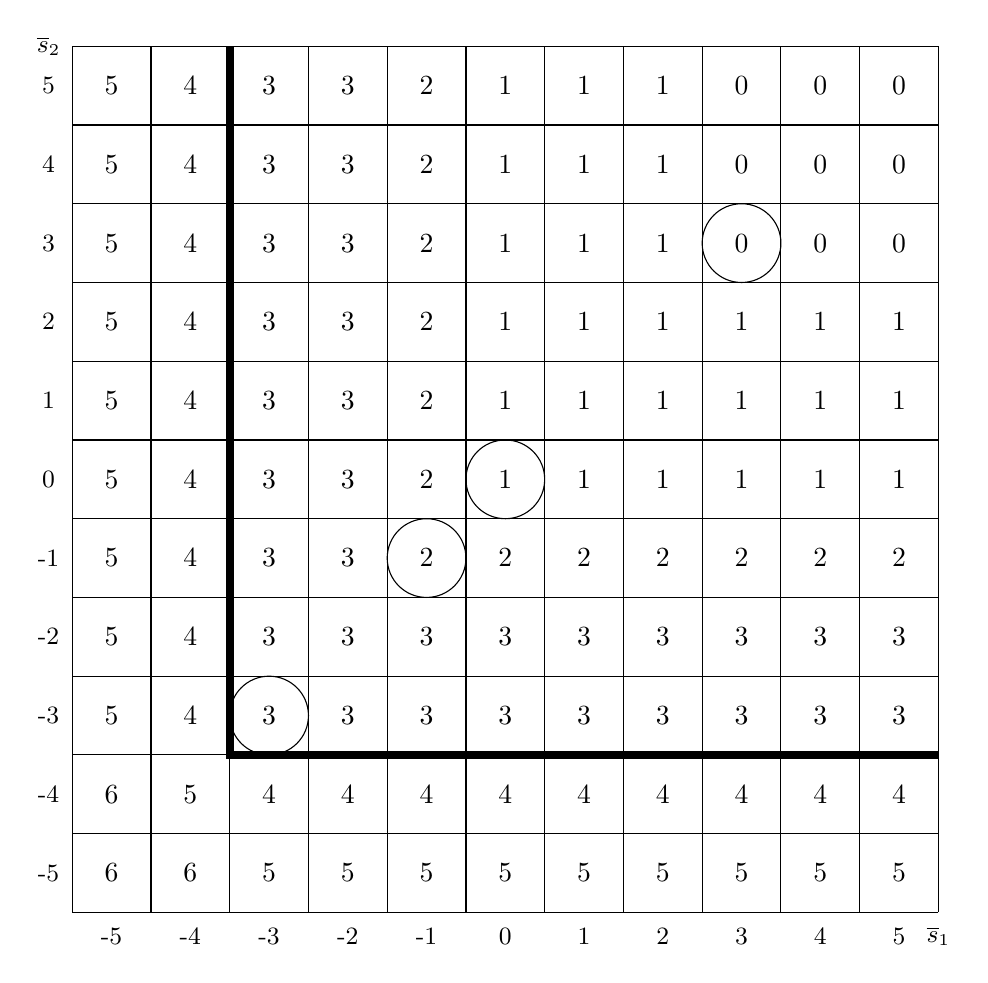
\begin{tikzpicture}
\draw[step=1] (0,0) grid (11,11);
\draw (11,-0.3) node {\small{$\overline{s}_1$}};
\draw (10.5,-0.3) node {\small{5}};
\draw (9.5,-0.3) node {\small{4}};
\draw (8.5,-0.3) node {\small{3}};
\draw (7.5,-0.3) node {\small{2}};
\draw (6.5,-0.3) node {\small{1}};
\draw (5.5,-0.3) node {\small{0}};
\draw (4.5,-0.3) node {\small{-1}};
\draw (3.5,-0.3) node {\small{-2}};
\draw (2.5,-0.3) node {\small{-3}};
\draw (1.5,-0.3) node {\small{-4}};
\draw (0.5,-0.3) node {\small{-5}};
\draw (-0.3,11) node {\small{$\overline{s}_2$}};
\draw (-0.3,10.5) node {\small{5}};
\draw (-0.3,9.5) node {\small{4}};
\draw (-0.3,8.5) node {\small{3}};
\draw (-0.3,7.5) node {\small{2}};
\draw (-0.3,6.5) node {\small{1}};
\draw (-0.3,5.5) node {\small{0}};
\draw (-0.3,4.5) node {\small{-1}};
\draw (-0.3,3.5) node {\small{-2}};
\draw (-0.3,2.5) node {\small{-3}};
\draw (-0.3,1.5) node {\small{-4}};
\draw (-0.3,0.5) node {\small{-5}};

\draw (10.5,10.5) node {0};
\draw (9.5,10.5) node {0};
\draw (8.5,10.5) node {0};
\draw (7.5,10.5) node {1};
\draw (6.5,10.5) node {1};
\draw (5.5,10.5) node {1};
\draw (4.5,10.5) node {2};
\draw (3.5,10.5) node {3};
\draw (2.5,10.5) node {3};
\draw (1.5,10.5) node {4};
\draw (0.5,10.5) node {5};

\draw (10.5,9.5) node {0};
\draw (9.5,9.5) node {0};
\draw (8.5,9.5) node {0};
\draw (7.5,9.5) node {1};
\draw (6.5,9.5) node {1};
\draw (5.5,9.5) node {1};
\draw (4.5,9.5) node {2};
\draw (3.5,9.5) node {3};
\draw (2.5,9.5) node {3};
\draw (1.5,9.5) node {4};
\draw (0.5,9.5) node {5};

\draw (10.5,8.5) node {0};
\draw (9.5,8.5) node {0};
\draw (8.5,8.5) node {0};
\draw (7.5,8.5) node {1};
\draw (6.5,8.5) node {1};
\draw (5.5,8.5) node {1};
\draw (4.5,8.5) node {2};
\draw (3.5,8.5) node {3};
\draw (2.5,8.5) node {3};
\draw (1.5,8.5) node {4};
\draw (0.5,8.5) node {5};


\draw (10.5,7.5) node {1};
\draw (9.5,7.5) node {1};
\draw (8.5,7.5) node {1};
\draw (7.5,7.5) node {1};
\draw (6.5,7.5) node {1};
\draw (5.5,7.5) node {1};
\draw (4.5,7.5) node {2};
\draw (3.5,7.5) node {3};
\draw (2.5,7.5) node {3};
\draw (1.5,7.5) node {4};
\draw (0.5,7.5) node {5};

\draw (10.5,6.5) node {1};
\draw (9.5,6.5) node {1};
\draw (8.5,6.5) node {1};
\draw (7.5,6.5) node {1};
\draw (6.5,6.5) node {1};
\draw (5.5,6.5) node {1};
\draw (4.5,6.5) node {2};
\draw (3.5,6.5) node {3};
\draw (2.5,6.5) node {3};
\draw (1.5,6.5) node {4};
\draw (0.5,6.5) node {5};

\draw (10.5,5.5) node {1};
\draw (9.5,5.5) node {1};
\draw (8.5,5.5) node {1};
\draw (7.5,5.5) node {1};
\draw (6.5,5.5) node {1};
\draw (5.5,5.5) node {1};
\draw (4.5,5.5) node {2};
\draw (3.5,5.5) node {3};
\draw (2.5,5.5) node {3};
\draw (1.5,5.5) node {4};
\draw (0.5,5.5) node {5};

\draw (10.5,4.5) node {2};
\draw (9.5,4.5) node {2};
\draw (8.5,4.5) node {2};
\draw (7.5,4.5) node {2};
\draw (6.5,4.5) node {2};
\draw (5.5,4.5) node {2};
\draw (4.5,4.5) node {2};
\draw (3.5,4.5) node {3};
\draw (2.5,4.5) node {3};
\draw (1.5,4.5) node {4};
\draw (0.5,4.5) node {5};

\draw (10.5,3.5) node {3};
\draw (9.5,3.5) node {3};
\draw (8.5,3.5) node {3};
\draw (7.5,3.5) node {3};
\draw (6.5,3.5) node {3};
\draw (5.5,3.5) node {3};
\draw (4.5,3.5) node {3};
\draw (3.5,3.5) node {3};
\draw (2.5,3.5) node {3};
\draw (1.5,3.5) node {4};
\draw (0.5,3.5) node {5};

\draw (10.5,2.5) node {3};
\draw (9.5,2.5) node {3};
\draw (8.5,2.5) node {3};
\draw (7.5,2.5) node {3};
\draw (6.5,2.5) node {3};
\draw (5.5,2.5) node {3};
\draw (4.5,2.5) node {3};
\draw (3.5,2.5) node {3};
\draw (2.5,2.5) node {3};
\draw (1.5,2.5) node {4};
\draw (0.5,2.5) node {5};

\draw (10.5,1.5) node {4};
\draw (9.5,1.5) node {4};
\draw (8.5,1.5) node {4};
\draw (7.5,1.5) node {4};
\draw (6.5,1.5) node {4};
\draw (5.5,1.5) node {4};
\draw (4.5,1.5) node {4};
\draw (3.5,1.5) node {4};
\draw (2.5,1.5) node {4};
\draw (1.5,1.5) node {5};
\draw (0.5,1.5) node {6};

\draw (10.5,0.5) node {5};
\draw (9.5,0.5) node {5};
\draw (8.5,0.5) node {5};
\draw (7.5,0.5) node {5};
\draw (6.5,0.5) node {5};
\draw (5.5,0.5) node {5};
\draw (4.5,0.5) node {5};
\draw (3.5,0.5) node {5};
\draw (2.5,0.5) node {5};
\draw (1.5,0.5) node {6};
\draw (0.5,0.5) node {6};

\draw[line width=3] (2,11)--(2,2)--(11,2);

\draw (8.5,8.5) circle (0.5);
\draw (5.5,5.5) circle (0.5);
\draw (4.5,4.5) circle (0.5);
\draw (2.5,2.5) circle (0.5);
\end{tikzpicture}
\end{center}

The stable range is given by $\overline{s}_1,\overline{s}_2\ge g(K)-m=3-6=-3,$
and the stable generators $\widetilde{z}_{\sigma_i}$ are marked by circles. 

For $m=7$ the $h$-function is very similar, except for
$$
h^{\stab}_{2,14}(-4,-4)=4,\
h^{\stab}_{2,14}(-4,-5)=h^{\stab}_{2,14}(-5,-4)=5,\ h^{\stab}_{2,14}(-5,-5)=6,
$$
and there is another stable generator $\widetilde{z}_{-4}$ with $\gr_{\w}(\widetilde{z}_{-4})=-8$.

For $m\ge 8$ we get
$$
h^{\stab}_{2,2m}(-4,-4)=4,\
h^{\stab}_{2,2m}(-4,-5)=h^{\stab}_{2,14}(-5,-4)=5,\ h^{\stab}_{2,2m}(-5,-5)=5,
$$
and there are stable generators $\widetilde{z}_{-4}$, $\widetilde{z}_{-5}$ with with $\gr_{\w}(\widetilde{z}_{-4})=-8,\gr_{\w}(\widetilde{z}_{-5})=-10$.
The stable relations between $\widetilde{z}_{\sigma_i}$ can be written in two ways:

1) Following \cite{BLZ} and Theorem \ref{thm: colored L space}, we can compute for $m\ge 6$:
$$
U_1\widetilde{z}_{3}=V_2(V_1V_2)^2\widetilde{z}_{0},\quad U_2\widetilde{z}_{3}=V_1(V_1V_2)^2\widetilde{z}_{0},
$$
$$
U_1\widetilde{z}_{0}=V_2\widetilde{z}_{-1},\quad U_2\widetilde{z}_{0}=V_1\widetilde{z}_{-1},
$$
$$
U_1\widetilde{z}_{-1}=V_2(V_1V_2)\widetilde{z}_{-3},\quad U_2\widetilde{z}_{-1}=V_1(V_1V_2)\widetilde{z}_{-3},
$$
For $m\ge 7$ we get additional relations
$$
U_1\widetilde{z}_{-3}=V_2\widetilde{z}_{-4},\quad U_2\widetilde{z}_{-3}=V_1\widetilde{z}_{-4},
$$
for $m\ge 8$ we get additional relations
$$
U_1\widetilde{z}_{-4}=V_2\widetilde{z}_{-5},\quad U_2\widetilde{z}_{-4}=V_1\widetilde{z}_{-5},
$$
and so on.

2) Following Lemma \ref{lem: A action}, we can instead describe the action of $\AAA$. For $m\ge 6$ we get 
\begin{equation}
\label{eq: T34 cable A relations}
\AAA\widetilde{z}_3=(V_1V_2)^2\widetilde{z}_0,\ 
\AAA\widetilde{z}_0=\widetilde{z}_{-1},\
\AAA\widetilde{z}_{-1}=(V_1V_2)\widetilde{z}_{-3},\
\AAA\widetilde{z}_{-3}=\widetilde{z}_{-4},\
\AAA\widetilde{z}_{-4}=\widetilde{z}_{-5}.
\end{equation}
The last two relations make sense for $m\ge 7$ and $m\ge 8$ respectively. Then all of the above relations are determined by \eqref{eq: T34 cable A relations} and
$
U_1=\AAA V_2,\ U_2=\AAA V_1.
$
Finally, note that \eqref{eq: T34 cable A relations} can be obtained from \eqref{eq: T34 relations} by changing $z_i$ to $\widetilde{z}_i$, $U$ to $\AAA$ and $V$ to $V_1V_2$, in agreement with Theorem \ref{thm: colored tensor product}.
 
%\EG{Finish this}
%\end{example}

\section{Application: crossing change maps}

Suppose two knot diagrams $K^+$ and $K^-$ differ at a single crossing which is positive in $K^+$ and negative in $K^-$. We would like to find a relation between their colored homologies, but first we relate the homology of cables. 

The blackboard framings for both $K^+$ and $K^-$ correspond to the writhe of their diagrams. Note that the writhe of $K^+$ is 2 more than the writhe of $K^-$.  The $n$-component cables of $K^+$ and $K^-$ are related by $n^2$ crossing changes. More precisely, changing $n^2$ negative crossings in $K^-_{n,mn}$ to positive results in $K^+_{n,(m+2)n}$ since the linking number between each pair of components increases by 2.

%\EG{Define the compatible framings on $K^-$ and $K^+$ and check whether we have same $m$ or $m+2$}
 


\begin{lemma}
\label{lem: big blowdown}
For $j\in \Z$ there is a map 
$$
G_{j,m}: \cHFL\left(K^-_{n,mn}\right)\to \cHFL\left(K^+_{n,(m+4)n}\right)
$$
of Maslov degree $-j^2-j$ and Alexander degree $A_i(G_{j,m})=-2j-1+2n,\ i=1,\ldots,n$. Furthermore, the maps $G_{j,m}$ commute with the connecting maps $\phi_k$:
$$
\begin{tikzcd}
\cHFL\left(K^-_{n,mn}\right) \arrow{r}{\phi_k} \arrow{d}{G_{j,m}}& \cHFL\left(K^-_{n,(m+1)n}\right) \arrow{d}{G_{j,m+1}}\\
\cHFL\left(K^+_{n,(m+4)n}\right) \arrow{r}{\phi_k}& \cHFL\left(K^+_{n,(m+5)n}\right).
\end{tikzcd}
$$
\end{lemma}

\begin{proof}
Consider the following braids on $2n$ strands: $\FT_{[1,n]}$ is the full twist on the left $n$ strands, $\FT_{[n+1,2n]}$ is the full twist on the right $n$ strands, and $\FT_{[1,2n]}$ is the full twist on all strands. Furthermore, consider the ``positive cabled crossing" braid $\beta_{n,n}$ which is the positive braid lift of the permutation $[n+1,\ldots,2n,1,\ldots,n]$:
\begin{center}
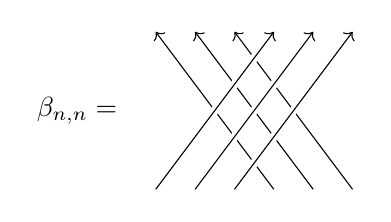
\begin{tikzpicture}
\draw (-1,1) node {$\beta_{n,n}=$};
\draw[->] (1.5,0)--(0,2);
\draw[->] (2,0)--(0.5,2);
\draw[->] (2.5,0)--(1,2);

\draw[->,line width=3,white] (0,0)--(1.5,2);
\draw[->,line width=3,white] (0.5,0)--(2,2);
\draw[->,line width=3,white] (1,0)--(2.5,2);
\draw[->] (0,0)--(1.5,2);
\draw[->] (0.5,0)--(2,2);
\draw[->] (1,0)--(2.5,2);
\end{tikzpicture}
\end{center}
It is easy to see that 
$
\FT_{[1,2n]}=\FT_{[1,n]}\FT_{[n+1,2n]}\beta_{n,n}^2$, and so $  \FT_{[1,2n]}\beta_{n,n}^{-1}=\FT_{[1,n]}\FT_{[n+1,2n]}\beta_{n,n}
$, that is: 
%\AA{Do we need to change the order to match the figure?}
\begin{center}
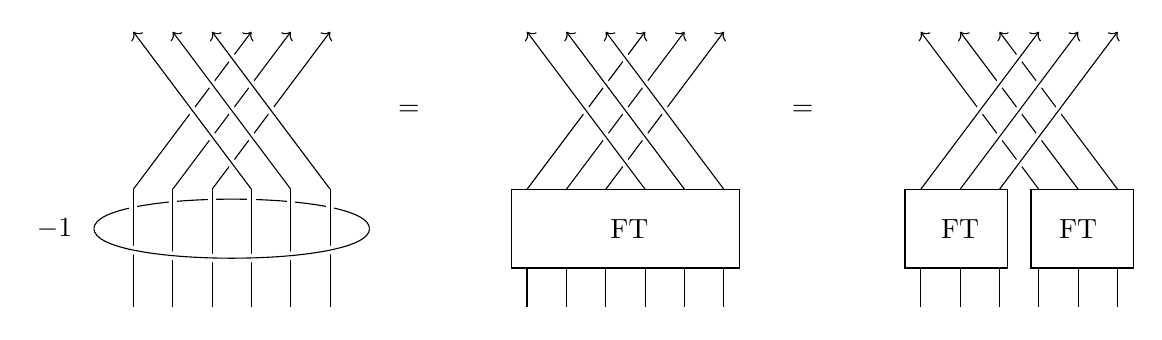
\begin{tikzpicture}
\draw[->] (-5,0)--(-3.5,2);
\draw[->] (-4.5,0)--(-3,2);
\draw[->] (-4,0)--(-2.5,2);

\draw[->,line width=3,white] (-3.5,0)--(-5,2);
\draw[->,line width=3,white] (-3,0)--(-4.5,2);
\draw[->,line width=3,white] (-2.5,0)--(-4,2);
\draw[->] (-3.5,0)--(-5,2);
\draw[->] (-3,0)--(-4.5,2);
\draw[->] (-2.5,0)--(-4,2);

\draw (-5.5,-0.5)..controls (-5.5,0) and (-2,0)..(-2,-0.5);

\draw[line width=3,white] (-5,-1.5)--(-5,0);
\draw[line width=3,white] (-4.5,-1.5)--(-4.5,0);
\draw[line width=3,white] (-4,-1.5)--(-4,0);
\draw[line width=3,white] (-3.5,-1.5)--(-3.5,0);
\draw[line width=3,white] (-3,-1.5)--(-3,0);
\draw[line width=3,white] (-2.5,-1.5)--(-2.5,0);

\draw (-5,-1.5)--(-5,0);
\draw (-4.5,-1.5)--(-4.5,0);
\draw (-4,-1.5)--(-4,0);
\draw (-3.5,-1.5)--(-3.5,0);
\draw (-3,-1.5)--(-3,0);
\draw (-2.5,-1.5)--(-2.5,0);

\draw[line width=3,white] (-5.5,-0.5)..controls (-5.5,-1) and (-2,-1)..(-2,-0.5);
\draw (-5.5,-0.5)..controls (-5.5,-1) and (-2,-1)..(-2,-0.5);

\draw (-6,-0.5) node {$-1$};

\draw (-1.5,1) node {$=$};
 
 

\draw[->] (0,0)--(1.5,2);
\draw[->] (0.5,0)--(2,2);
\draw[->] (1,0)--(2.5,2);

\draw[->,line width=3,white] (1.5,0)--(0,2);
\draw[->,line width=3,white] (2,0)--(0.5,2);
\draw[->,line width=3,white] (2.5,0)--(1,2);
\draw[->] (1.5,0)--(0,2);
\draw[->] (2,0)--(0.5,2);
\draw[->] (2.5,0)--(1,2);

\draw (-0.2,0)--(2.7,0)--(2.7,-1)--(-0.2,-1)--(-0.2,0);
\draw (0,-1)--(0,-1.5);
\draw (0.5,-1)--(0.5,-1.5);
\draw (1,-1)--(1,-1.5);
\draw (1.5,-1)--(1.5,-1.5);
\draw (2,-1)--(2,-1.5);
\draw (2.5,-1)--(2.5,-1.5);
\draw (1.3,-0.5) node {$\FT$};

\draw (3.5,1) node {$=$};
 
\draw[->] (6.5,0)--(5,2);
\draw[->] (7,0)--(5.5,2);
\draw[->] (7.5,0)--(6,2);

\draw[->,line width=3,white] (5,0)--(6.5,2);
\draw[->,line width=3,white] (5.5,0)--(7,2);
\draw[->,line width=3,white] (6,0)--(7.5,2);
\draw[->] (5,0)--(6.5,2);
\draw[->] (5.5,0)--(7,2);
\draw[->] (6,0)--(7.5,2);

\draw (4.8,0)--(6.1,0)--(6.1,-1)--(4.8,-1)--(4.8,0);
\draw (6.4,0)--(7.7,0)--(7.7,-1)--(6.4,-1)--(6.4,0);
\draw (5,-1)--(5,-1.5);
\draw (5.5,-1)--(5.5,-1.5);
\draw (6,-1)--(6,-1.5);
\draw (6.5,-1)--(6.5,-1.5);
\draw (7,-1)--(7,-1.5);
\draw (7.5,-1)--(7.5,-1.5);
\draw (5.5,-0.5) node {$\FT$};
\draw (7,-0.5) node {$\FT$};
\end{tikzpicture}
\end{center}
This means that adding a full twist  to $K^{-}_{n,mn}$ results in $K^{+}_{n,(m+2)n}$ with two additional full twists which is isotopic to $K^{+}_{n,(m+4)n}$. Now the construction of $G_{j,m}$ follows from \cite[Proposition 3.10]{AGL}, this also gives the Maslov grading change.

For the Alexander grading we use equation \eqref{eq: Alexander shift generalized}. Let $M$ be the $(-1)$-framed unknot. Since $\lk(K^{-}_{n, mn},M)=2n$ and $\lk(L_i,M)=2$ for each component $L_i$, we get
$$
A_i=\frac{1}{2}\left[-2j-1+2n\right]\cdot 2=-2j-1+2n.
$$

The cobordism defining $\phi_k$ corresponds to blowing down a meridian of $K^{-}_{n,mn}$ (resp. $K^+_{n,(m+4)n}$) which can be done away from the crossing, and therefore the two cobordisms commute and induced maps in Heegaard Floer homology commute.  
\end{proof}

\begin{lemma}
\label{lem: big blowdown 2}
For $j\in \Z$ there is a map 
$$
F_{j,m}: \cHFL\left(K^+_{n,mn}\right)\to \cHFL\left(K^-_{n,(m-2)n}\right)
$$
of Maslov degree $-j^2-j$ and Alexander degree $A_i=0$. Furthermore, the maps $F_{j,m}$ commute with the connecting maps $\phi_k$:
$$
\begin{tikzcd}
\cHFL\left(K^+_{n,mn}\right) \arrow{r}{\phi_k} \arrow{d}{F_{j,m}}& \cHFL\left(K^+_{n,(m+1)n}\right) \arrow{d}{F_{j,m+1}}\\
\cHFL\left(K^-_{n,(m-2)n}\right) \arrow{r}{\phi_k}& \cHFL\left(K^-_{n,(m-1)n}\right).
\end{tikzcd}
$$
\end{lemma}

\begin{proof}
The proof is similar to the proof of Lemma \ref{lem: big blowdown}, where we now use the following diagram (compare with \cite[Proposition 3.1]{AGL}):
\begin{center}
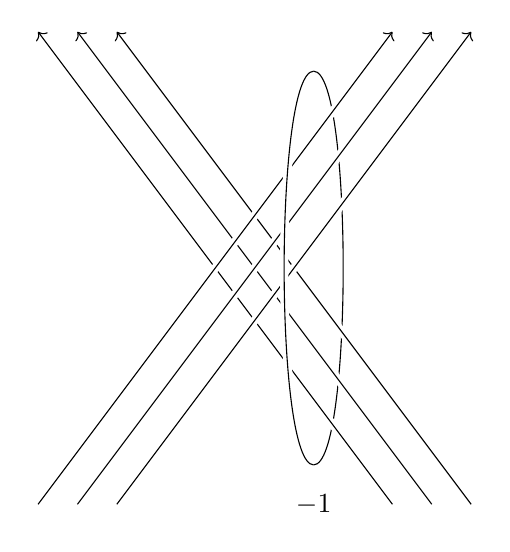
\begin{tikzpicture}
\draw (-3,-1.5)..controls (-2.5,-1.5) and (-2.5,3.5)..(-3,3.5);

\draw[->,line width=3,white] (-2,-2)--(-6.5,4);
\draw[->,line width=3,white] (-1.5,-2)--(-6,4);
\draw[->,line width=3,white] (-1,-2)--(-5.5,4);
\draw[->] (-2,-2)--(-6.5,4);
\draw[->] (-1.5,-2)--(-6,4);
\draw[->] (-1,-2)--(-5.5,4);

\draw[->,line width=3,white] (-6.5,-2)--(-2,4);
\draw[->,line width=3,white] (-6,-2)--(-1.5,4);
\draw[->,line width=3,white] (-5.5,-2)--(-1,4);

\draw[->] (-6.5,-2)--(-2,4);
\draw[->] (-6,-2)--(-1.5,4);
\draw[->] (-5.5,-2)--(-1,4);



\draw[line width=3,white]  (-3,-1.5)..controls (-3.5,-1.5) and (-3.5,3.5)..(-3,3.5);

\draw (-3,-1.5)..controls (-3.5,-1.5) and (-3.5,3.5)..(-3,3.5);


\draw (-3,-2) node {$-1$};

  
\end{tikzpicture}
\end{center}
Blowing down the circle changes the positive cabled crossing in $K^+_{n,mn}$ to the negative one (resulting in $K^-_{n,(m-2)n}$), introduces a positive full twist on one set of $n$ strands and a negative full twist on the second set of $n$ strands. Since $K$ is connected, we can slide the full twists along $K$ and cancel with each other. As a result, we are left with $K^-_{n,(m-2)n}$. 

For the Alexander degree, we denote the $(-1)$-framed unknot by $M$, and  use \eqref{eq: Alexander shift generalized} again. We have $\lk(L_i,M)=0$ for all component $L_i$ of $K^+_{n, mn}$, so the Alexander grading does not change. 
 \end{proof}

\begin{theorem}
a) The maps $G_{j,m}$ induce maps 
$$
G_j:\Cab_n(K^{-})\to \Cab_n(K^+),\ \gr_{\w}(G_j)=-j^2-j,\ A_i(G_j)=-2j-1+2n
$$ 
of twist degree $4$ which commute with the action of the cable algebra $\CA_n$. 

b) We obtain maps 
$$
G_j^{\col}:\CH_n(K^{-})\to \CH_n(K^+),\ \gr_{\w}(G_j^{\col})=-j^2-j,\ A_i(G_j^{\col})=-2j+1
$$
which commute with the action of the algebra $\CA_n^{\col}$.

c) The maps $F_{j,m}$ induce maps 
$$
F_j:\Cab_n(K^{+})\to \Cab_n(K^-),\ \gr_{\w}(F_j)=-j^2-j,\ A_i(F_j)=0
$$ 
of twist degree $-2$ which commute with the action of the cable algebra $\CA_n$. 

d) We obtain maps 
$$
F_j^{\col}:\CH_n(K^{+})\to \CH_n(K^-),\ \gr_{\w}(F_j^{\col})=-j^2-j,\ A_i(F_j^{\col})=n-1
$$
which commute with the action of the algebra $\CA_n^{\col}$.
\end{theorem}



\begin{proof}
Part (a) is a restatement of Lemma \ref{lem: big blowdown}, and  (b) follows from (a) after regrading
$$
-2j-1+2n-(m+4)(n-1)/2+m(n-1)/2=-2j+1.
$$
Similarly, (c) follows from Lemma \ref{lem: big blowdown 2} and (d) follows from (c) after regrading
$$
0-(m-2)(n-1)/2+m(n-1)/2=n-1.
$$
\end{proof}

\begin{remark}
The cables $K^+_{n,(m+2)n}$ and $K^-_{n,mn}$ are related by a sequence of $n^2$ crossing changes, and we can instead consider compositions of local cobordisms maps at these crossings as in \cite[Section 5]{AGL}.

Let $Z\subset \{1,\ldots,n\}\times \{1,\ldots,n\}$ be an arbitrary subset. Then there exists a   map 
$$
\Psi_{Z,m}:\cHFL\left(K^+_{n,(m+2)n}\right)\to \cHFL\left(K^-_{n,mn}\right)
$$
of Maslov degree zero and Alexander degree 
$$
A(\Psi_{Z,m})=\frac{1}{2}\left(\sum_{(i,j)\in Z}(\ee_i-\ee_j)-\sum_{(i,j)\notin Z}(\ee_i-\ee_j)\right).
$$
It is easy to see that, as before, $\Psi_{Z,m}$ commutes with the connecting maps $\phi_k$, and hence defines a map $\CH_n(K^+)\to \CH_n(K^-)$.
\end{remark}

 


 

\begin{thebibliography}{99}

\bibitem{AGL} A. Alishahi, E. Gorsky, B. Liu. Splitting maps in link Floer homology and integer points in permutahedra. arXiv:2307.07741

\bibitem{BGHW} W. Ballinger, E. Gorsky, M. Hogancamp, J. Wang. Stable deformed $\mathfrak{gl}_N$ homology of torus knots. arXiv:2507.00175


\bibitem{BPRW}  A. Beliakova, K. Putyra, L.-H. Robert, E. Wagner. A proof of Dunfield-Gukov-Rasmussen Conjecture. J. Eur. Math. Soc. (2025), arXiv:2210.00878

\bibitem{BorodzikGorskyImmersed} M. Borodzik and E. Gorsky. Immersed concordances of links and Heegaard Floer homology. Indiana Univ. Math. J. 67 (2018), no. 3, 1039--1083. 



\bibitem{BLZ} M. Borodzik, B. Liu, I. Zemke. Lattice homology, formality,  and plumbed L-space links.  J. Eur. Math. Soc. (2024), arXiv:2210.15792

\bibitem{Chen} D. Chen, I. Zemke, H. Zhou. L-space satellite operators and knot Floer homology. arXiv:2412.05755

\bibitem{Cautis} S. Cautis. Clasp technology to knot homology via the affine Grassmannian. Mathematische Annalen 363 (2015): 1053--1115.

\bibitem{Conners} L. Conners. Row--column mirror symmetry for colored torus knot homology.
Selecta Mathematica 30 (5), article 97.

\bibitem{Cooper} B. Cooper, R. Deyeso.  Holonomicity from a Heegaard-Floer Perspective. arXiv:2501.01519

\bibitem{CK} B. Cooper, V. Krushkal. Categorification of the Jones--Wenzl projectors. Quantum Topology 3.2 (2012): 139--180.

\bibitem{DGR} N. Dunfield, S. Gukov, J. Rasmussen. The superpolynomial for knot homologies. Experimental Mathematics 15.2 (2006): 129--159.

\bibitem{GHog} E. Gorsky, M. Hogancamp. Hilbert schemes and  $y$-ification of Khovanov-Rozansky homology.
Geom. Topol. 26 (2022), no. 2, 587--678.

\bibitem{GH} E. Gorsky, J. Hom. Cable links and L-space surgeries.  
Quantum Topology 8 (2017), no.4, 629--666.

\bibitem{GNR} E. Gorsky, A. Negu\cb{t}, J. Rasmussen. Flag Hilbert schemes, colored projectors and Khovanov-Rozansky homology. Advances in Mathematics 378 (2021): 107542.

\bibitem{GOR} E. Gorsky, A. Oblomkov, J. Rasmussen. On stable Khovanov homology of torus knots. Experimental Mathematics 22.3 (2013): 265--281.

\bibitem{Hedden} M. Hedden. On knot Floer homology and cabling
Algebraic \& Geometric Topology 5 (2005), 1197--1222.

\bibitem{Hedden2}  M. Hedden. On knot Floer homology and cabling. II.
International Mathematics Research Notices, 2009, no. 12, 2248--2274.

\bibitem{Hogancamp} 
M. Hogancamp. Categorified Young symmetrizers and stable homology of torus links.
Geometry \& Topology 22 (2018) 2943--3002.

\bibitem{Hogancamp2} M. Hogancamp. A polynomial action on colored  $\mathfrak{sl}_2$  link homology.
Quantum Topol. 10 (2019), no. 1, 1--75.


\bibitem{Kh}  M. Khovanov. A categorification of the Jones polynomial.
Duke Math. J. 101 (2000), no. 3, 359--426.

\bibitem{KR1} M. Khovanov, L. Rozansky. Matrix factorizations and link homology.
Fund. Math. 199 (2008), no. 1, 1--91.

\bibitem{KR2}  M. Khovanov, L. Rozansky. Matrix factorizations and link homology. II
Geom. Topol. 12 (2008), no. 3, 1387--1425.


\bibitem{Licata} J. Licata. Heegaard Floer homology of $(n,n)$-torus links: computations and questions.  arXiv:1208.0394.

\bibitem{Lipshitz-cylindrical} R. Lipshitz. A cylindrical reformulation of Heegaard Floer homology. Geom. Topol. 10 (2006) 955-1096.

\bibitem{Yajing} Y. Liu. L-space surgeries on links. Quantum Topol. 8 (2017), no. 3, 505--570.

\bibitem{MM} P. Melvin, H. Morton. The coloured Jones function. Comm. Math. Phys. 169 (1995), no. 3, 501--520.



\bibitem{OSKnots} P. Ozsv\'ath, Z. Szab\'o. Holomorphic disks and knot invariants. Adv. Math. 186 (2004), no.1, 58--116. 



\bibitem{OSProperties} P. Ozsv\'ath, Z. Szab\'o. Holomorphic disks and three-manifold invariants: properties  and applications. Ann. of Math. (2) 159 (2004), no.3, 1159--1245. 

\bibitem{OSlens} P. Ozsv\'ath, Z. Szab\'o. On knot Floer homology and lens space surgeries. Topology 44 (2005), no.6, 1281--1300.


\bibitem{OSLinks} P. Ozsv\'ath, Z. Szab\'o. Holomorphic disks, link invariants and the multi-variable  Alexander polynomial. Algebr. Geom. Topol. 8 (2008), no. 2, 615--692.

\bibitem{RasmussenKnots} J. Rasmussen. Floer homology and knot complements. PhD thesis, Harvard University, 2003.



\bibitem{RasDiff} J. Rasmussen. Some differentials on Khovanov–Rozansky homology. Geometry \& Topology, 19(6), 3031--3104.

\bibitem{RT}  N. Y. Reshetikhin and V. G. Turaev. Ribbon graphs and their invariants derived from
quantum groups. Comm. Math. Phys. 127 (1990), 1--26.

\bibitem{RJ} M. Rosso and V. F. R. Jones. On the invariants of torus knots derived from quantum groups. Journal of Knot Theory and its 
Ramifications 2 (1993), 97--112.

\bibitem{Rozansky} L. Rozansky. An infinite torus braid yields a categorified Jones--Wenzl projector. Fundamenta Mathematicae 225 (2014): 305--326.

\bibitem{Wildi} A. Wildi. On Categorifications and Applications of Knot Invariants. PhD thesis, University of Z\"urich, 2025.

%\bibitem{Willis}

\bibitem{Zemke:graph} I. Zemke. Graph cobordisms and Heegaard Floer homology. arXiv:1512.01184.

\bibitem{Zemke} I. Zemke. Link cobordisms and functoriality in link Floer homology. J. Topol. 12 (2019), no. 1, 94--220. 

\bibitem{Zemke2} I. Zemke. Link cobordisms and absolute gradings on link Floer homology. Quantum Topol. 10 (2019), no. 2, 207--323. 

\bibitem{Zemke:basepoint} I. Zemke. Quasistabilization and basepoint moving maps in link Floer homology. Algebraic \& Geometric Topology 17 (2017), no. 6, 3461 -- 3518.

\bibitem{Zemke:bordered} I. Zemke. Bordered manifolds with torus boundary and the link surgery formula. arXiv:2109.11520.


\end{thebibliography}


\end{document}
)
